\documentclass[pdftex,dvipsnames]{dissertation}

% --- Encoding stuff ----------------------------------------------------------
\usepackage[utf8]{inputenc}
\usepackage[T1]{fontenc}

% --- English stuff -----------------------------------------------------------
\usepackage[french,english]{babel}
% \usepackage[english]{babel}
\selectlanguage{english}

\usepackage{xspace}
\usepackage{csquotes}

% --- Debug stuff -------------------------------------------------------------
\usepackage{morewrites} % workaround for "no room for new \write" error

% --- Font stuff --------------------------------------------------------------
\usepackage{stackengine} % for overlapping text

% --- Appendices --------------------------------------------------------------

% --- Blind text --------------------------------------------------------------
\usepackage{blindtext} % provide \blindtext, \Blindtext
\usepackage{lipsum}

\usepackage{xargs}   % Use more than one optional parameter in a new commands
\usepackage{xcolor}  % Coloured text etc.

% --- TODO notes --------------------------------------------------------------
\usepackage[colorinlistoftodos,prependcaption,textsize=small,shadow]{todonotes}
% my alias
\input{utils/todonotes}

% --- Symbols, Units and Icons ------------------------------------------------
\usepackage{fontawesome} % fontawesomeicons
\usepackage{arydshln} % provide dashline
\usepackage{pifont}% http://ctan.org/pkg/pifont
\usepackage{gensymb} % provide \degree

% --- Math --------------------------------------------------------------------
\usepackage{kmath} % cool delimiters
\usepackage{dsfont} % double stroke
\usepackage[mathscr]{euscript}
\usepackage{xfrac} % provide \sfrac, cool fractions
\usepackage{siunitx}    % provide \ang and SI units
\usepackage{epsdice} % provide \epsdice

% --- Theorem environment------------------------------------------------------
\usepackage{amsthm}
\usepackage{thmtools}
\usepackage{thm-restate}
\declaretheorem[%
    name=Rationale,
    refname={Rationale,Rationales},
    Refname={Rationale,Rationales}
]{rationale}
\declaretheorem[%
    name={Security Claim},
    numbered={unless unique},
]{secclaim}

% --- Packages from Frederich -------------------------------------------------
\usepackage{longtable}
\usepackage{pdflscape}
\usepackage{enumitem}

%%% OTHER INCLUDES
\newrobustcmd*{\fullfullcite}{%
    \AtNextCite{%
        \AtEachCitekey{%
            \defcounter{maxnames}{99}%
            \DeclareNameAlias{labelname}{given-family}%
        }%
    }%
    \fullcite
}

%% IMAGE AS SYMBOL

% % set the Bison QED symbol
% \renewcommand{\qed}{%
% \leavevmode\unskip\penalty9999 \hbox{}\nobreak\hfill%
% \quad\hbox{\includegraphics[height=1em]{bison/bison-qed.jpg}}}

\newcommand{\cpother}[1]{{\color{BlueGreen} #1}}
\newcommand{\cpmine}[1]{{\color{GreenYellow} #1}}

% --- my abbreviation ---------------------------------------------------------
\newcommand{\imgsrc}[1]{Image courtesy of #1}
\newcommand{\cfr}[1]{\Cf/ #1}

% --- math models -------------------------------------------------------------
\newcommand{\echoModelFreq}{\ensuremath{
    H_{ij}(f_k) = \sum_{\idxEch=0}^{\numEchs}
        \frac{\absCoeff_{ij}^r}{4 \pi \speedOfSound \tau_{ij}^r}
        \cste^{- \csti 2 \pi k \Fs \tau_{ij}^r / F}}}

\newcommand{\sumEcho}{\ensuremath{\sum_{\idxEch=0}^{\numEchs}}}
\newcommand{\echoModelTimeSimple}[1]{\ensuremath{\sumEcho \alpha_{#1}^{(r)} \delta(t - \tau_{#1}^{(r)})}}
\newcommand{\alltaus}[1]{\ensuremath{\{\tau_{#1}^{(r)}\}_{#1,r}}}
\newcommand{\allalphas}[1]{\ensuremath{\{\alpha_{#1}^{(r)}\}_{#1,r}}}

\newcommand{\icon}[1]{\raisebox{-.1\height}{\includegraphics[height=3ex]{#1}}}
\newcommand{\chaosIcon}{\icon{figures/blaster/chaos.png}}
% notation
\newcommand{\idxSrcs}{\ensuremath{i}}
\newcommand{\idxMics}{\ensuremath{j}}
\newcommand{\numSrcs}{\ensuremath{I}}
\newcommand{\numMics}{\ensuremath{J}}

\newcommand{\positionMicrophone}{\ensuremath{\undeline{\mathbf{x}}}}
\newcommand{\positionSource}{\ensuremath{\undeline{\mathbf{s}}}}

\newcommand{\contMicrophoneSignal}{\ensuremath{x}}
\newcommand{\contSource}{\ensuremath{s}}

\newcommand{\contRIR}{\ensuremath{h}}
\newcommand{\contNoise}{\ensuremath{n}}

% % algos names:
% \newcommand{\lantern}{\textsc{Lantern}}
\newcommand{\mirage}{\textsc{Mirage}}
\newcommand{\separake}{\textsc{Separake}}
\newcommand{\brioche}{\textsc{Brioche}}
% \newcommand{\blaster}{\textsc{Blaster}}
% \newcommand{\blasterr}{\textsc{Blasterr}}

%----------------
\usepackage{pgffor}
\foreach \x in {a,...,z}{
  % mathbf
  \expandafter\xdef\csname bf\x \endcsname{\noexpand\ensuremath{\noexpand\mathbf{\x}}}
  % Bold symbol
  \expandafter\xdef\csname bs\x \endcsname{\noexpand\ensuremath{\noexpand\boldsymbol{\x}}}
}

\foreach \x in {A,...,Z}{
%   % Bold symbol
  \expandafter\xdef\csname bs\x \endcsname{\noexpand\ensuremath{\noexpand\boldsymbol{\x}}}
%   % mathbf
  \expandafter\xdef\csname bf\x \endcsname{\noexpand\ensuremath{\noexpand\mathbf{\x}}}
%   % mathbb
  \expandafter\xdef\csname bb\x \endcsname{\noexpand\ensuremath{\noexpand\mathbb{\x}}}
%   % mathds
  \expandafter\xdef\csname ds\x \endcsname{\noexpand\ensuremath{\noexpand\mathds{\x}}}
%   % mathcal
  \expandafter\xdef\csname cal\x \endcsname{\noexpand\ensuremath{\noexpand\mathcal{\x}}}
}

%%% MACROS
\newcommand{\gc}[1]{{\textcolor{green}{#1}}}
% \newcommand{\gc}[1]{{\textcolor{black}{#1}}}

\newcommand{\gccor}[2]{{\textcolor{red}{[#1 $\rightarrow$ #2]}}}
% \newcommand{\gccor}[2]{{\textcolor{black}{#2}}}

\newcommand{\gccmt}[1]{{\textcolor{blue}{[SE: #1]}}}
%\newcommand{\gccmt}[1]{}

\newcommand{\gcrm}[1]{{\textcolor{magenta}{[#1]}}}
% \newcommand{\gcrm}[1]{{\textcolor{black}{}}}

% --- Table of Contents -------------------------------------------------------
%%% TOC STYLE : check in the dissertation class
% check dissertation class
% %% MINITOC per CHAPTER
\usepackage{minitoc} % must be inserted after any modification of TOC

% --- Graphics ----------------------------------------------------------------
\usepackage{pgfplots}
\pgfplotsset{compat=1.8}
\usepgfplotslibrary{fillbetween} %for fill under curve
\usepackage{tikz}
\usetikzlibrary{calc,patterns,arrows,shapes.arrows,intersections,fadings,shadows.blur}
\usepackage[abs]{overpic}
% \usepackage[percent]{overpic} % provide \put on figures
\graphicspath{{./figures/}{./icons/}{./logos/}}
\DeclareGraphicsExtensions{.pdf,.png,.jpg}
% add pdf pages
\usepackage{pdfpages} % \includepdf[pages=-]{myfile.pdf}
\usepackage{rotating} % provide sidewaystable env
% 2 sub figures
% \usepackage{subcaption}
% \pgfplotsset{%
%     table/search path={./figures/plots/},
% }

% --- Algorithm ---------------------------------------------------------------
\newcommand\mycommfont[1]{\footnotesize\ttfamily\textbf{\textcolor{mygray}{#1}}}
\SetCommentSty{mycommfont}

% --- Bibliopgraphy -----------------------------------------------------------
\bibliography{contents/back_matter/references.bib, contents/back_matter/references_separake.bib, contents/back_matter/references_dechorate.bib}


% --- Include only ------------------------------------------------------------
\newcommand{\synopsisChAcoustics}{
    This chapter will build a first important bridge: from acoustics to audio signal processing.
    It first defines sound and how it propagates in the environment~\cref{ch:acoustics:sec:wave}, teasing out the fundamental concepts of this thesis: the echoes.~\cref{ch:acoustics:sec:reflection} and the \RIRdef/~\cref{ch:acoustics:sec:rir}.
    By assuming some approximations, the \RIR/ will be described in all its parts in relation with methods to compute them.
    Finally, in~\cref{ch:acoustics:sec:perception}, how the human auditory system perceives reverberation will be reported.
}
\newcommand{\synopsisChProcessing}{
    Let us now move from the physics to digital signal processing.
    At first in~\cref{sec:processing:model}, this chapter formalizes fundamental concepts of audio signal processing such as signal, mixtures and noise in the time domain.
    In~\cref{sec:processing:domains}, we will present the signal representation that we will use throughout the entire thesis: the \STFTdef/.
    Finally, after assuming the narrowband approximation, in~\cref{sec:processing:rirmodels} some important models for the \RIRdef/ are described.
}
\newcommand{\synopsisChEstimation}{
This chapter amis to provide the reader with knowledge of the state-of-the-art of \AERdef/.
After presenting the \AER/ problem in~\cref{sec:estimation:problem}, the chapter is divided into three main sections:
\cref{sec:estimation:taxonomy} defines the categories of methods thank to which the literature can be clustered and analyzed in detail later in~\cref{sec:estimation:sota}.
Finally, in~\cref{sec:estimation:datametrics} some datasets and evaluation metrics for \AER/ are presented.
}

\newcommand{\synopsisChBlaster}{
This chapter proposes a novel approach for \textit{off-grid} \AER/ from a stereophonic recording of an unknown sound source such as speech.
In contrast with existing methods, the proposed approach, named \BLASTERdef/.
It is built on the recent framework of \CDdef/ and it does not rely on parameter tuning nor peak picking techniques by working directly in the parameter space of interest.
The accuracy and robustness of the method are assessed on challenging simulated setups with varying noise and reverberation levels and are compared to two state-of-the-art methods.
While comparable or slightly worse recovery rates are observed for the task of recovering 7 echoes or more, better results are obtained for fewer echoes and the off-grid nature of the approach yields generally smaller estimation errors.
}

\newcommand{\synopsisChLantern}{
    This chapter
}

\newcommand{\synopsisChSeparake}{
    In this chapter echoes are used for boosting the performances of state-of-the-art approaches in Audio Source Separation.
    At first, we describe the existing methods, which typically that either ignore the acoustic propagation, nor attempt to estimate it fully.
    % Instead, thanks to the geometric interpretation of early echoes, we show how this gives us enough spatial diversity to get a performance boost over the anechoic case.
    Instead, this works investigate whether sound separation can benefit of the knowledge of acoustic echoes derived from know the locations of a few virtual microphones.
    The improvements are show for two standard algorithms based on non-negative matrix factorization: one that uses only magnitudes of the transfer functions, and one that also uses the phases.
    The experimental part shows that the proposed approach based on a few echoes beats its vanilla variant, and that with magnitude information only, echoes enable separation where it was previously impossible.
}

\newcommand{\synopsisChDechorate}{
    This chapter presents \dEchorate{}: a new database of measured multichannel room impulse response (RIRs) including annotations of early echoes and 3D positions of microphones, real and image sources under different wall configurations in a cuboid room.
    These data provide a tool for benchmarking recent methods in \textit{echo-aware} speech enhancement, room geometry estimation, RIR estimation, acoustic echo retrieval, microphone calibration, echo labeling and reflectors estimation.
    The database is accompanied with software utilities to easily access, manipulate and visualize the data as well as baseline methods for echo-related tasks.
}



\includeonly{   % Of course this list allows many more file
%  intro,       % should also work with files in different paths
    contents/front_matter/abstract,
    contents/front_matter/resume,
    % contents/front_matter/resume_etendu_fr,
    % contents/front_matter/acknowledgments,
    contents/front_matter/glossary,
    % contents/front_matter/notation,
    % contents/main_matter/chapter0_intro,
    % contents/main_matter/chapter1_acoustics,
    % contents/main_matter/chapter2_processing
    contents/main_matter/chapter_estimation,
    % contents/main_matter/chapter_blaster,
    % contents/main_matter/chapter_lantern,
    % contents/main_matter/chapter_dechorate,
    % contents/main_matter/chapter9_applications,
    % contents/main_matter/chapter_separake,
    % contents/main_matter/chapter11_mirage,
    % contents/main_matter/chapter_dechorateapp,
    % contents/main_matter/chapter20_conclusion,
    contents/back_matter/bibliography,
}

%%%%%%%%%%%%%%%%%%%%%%%%%%%%%%%%%%%%%%%%%%%%%%%%%%%%%%%%%%%%%%%%%%%%%%%%%%%%%%%
%%%%%%%%%%%%%%%%%%%%%%%%%%%%%%%%%%DOCUMENT%%%%%%%%%%%%%%%%%%%%%%%%%%%%%%%%%%%%%
%%%%%%%%%%%%%%%%%%%%%%%%%%%%%%%%%%%%%%%%%%%%%%%%%%%%%%%%%%%%%%%%%%%%%%%%%%%%%%%

\title{Hunting Acoustic Echoes for Auditory Scene Analysis}
\author{Diego DI CARLO}
\date{\today}

\begin{document}
\frontmatter{}

% % front matter / titelei
% recto: halftitlepage / schmutztitelseite, vortitel
\thispagestyle{empty}
{
    \begin{fullwidth}
        \centering
        \hphantom{.}
        \vfill
        {\Huge
            Hunting Echoes\\
            for\\
            Auditory Scene Analysis
        }
        \vfill
        \vfill
    \end{fullwidth}
}

\clearpage{}

% verso: frontispiece / frontiszipzseite, vakatseite
% dedication
\cleardoublepage{}

% recto: titlepage / titelblatt, innentitel
\thispagestyle{empty}
{
    \calccentering{\unitlength}
    \begin{adjustwidth*}{\unitlength}{-\unitlength}
        \raggedleft{}
        {\Huge\color{Burgundy}%
        Hunting Echoes\\
        for Auditory Scene Analysis}\\[\baselineskip]
        {\LARGE%
        Dissertation Thesis}\\[0.2\textheight]
        {\huge%
        Diego \textsc{Di Carlo}}\\[\baselineskip]
        {\LARGE%
        \today}
        \vfill
        \vfill
        {\large%
        Submitted in partial fulfillment of the requirements\\
        for the degree of Doktor der Naturwissenschaften\\[\baselineskip]% (Dr.\ rer.\ nat.)\\[\baselineskip]

        to the\\[\baselineskip]

        Faculty of Mathematics\\
        at Ruhr-Universität Bochum\\[2\baselineskip]
        %Vorgelegt zur Erlangung des\\
        %Doktorgrades der Naturwissenschaften\\
        %an der Fakultät der Mathematik\\
        %der Ruhr-Universität Bochum\\[2\baselineskip]

        \begin{minipage}{0.5\textwidth}
        \begin{tabular}{lr}
            1st\hspace{4pt} Reviewer & Prof.\ Dr. Gregor Leander\\
            2nd Reviewer & Prof.\ Dr.\; Alexander May
        \end{tabular}
        \end{minipage}
        \hspace*{36pt}
        %}\hspace*{-8pt}

        %\vspace{2\baselineskip}
        %Datum der Disputation: 13.\ Dezember 2019
        \vfill
        }
        \vspace*{\baselineskip}
    \end{adjustwidth*}
}

\clearpage{}

% verso: colophon / impressum
\thispagestyle{empty}
\hphantom{.}
\vfill

\section*{Imprint}

\textit{Hunting Echoes for Audtory Scene Analysis}\\
Copyright \textcopyright{} 2020 by \theauthor{}.\\
All rights reserved. Printed in France.\\
Published by the Ruhr-Universität Bochum, Bochum, Germany.

\section*{Colophon}

This thesis was typeset using \LaTeX{} and the \texttt{memoir} documentclass.
It is based on Aaron Turon's thesis \emph{Understanding and expressing scalable concurrency}\footnote{\url{https://people.mpi-sws.org/~turon/turon-thesis.pdf}}, itself a mixture of \texttt{classicthesis}\footnote{\url{https://bitbucket.org/amiede/classicthesis/}} by Andr\'e Miede and \texttt{tufte-latex}\footnote{\url{https://github.com/Tufte-LaTeX/tufte-latex}}, based on Edward Tufte's \emph{Beautiful Evidence}.\\[0.5\baselineskip]
%
The bibliography was processed by Biblatex.
All graphics and plots are made with PGF/Ti\emph{k}Z.\\[0.5\baselineskip]
%
The body text is set 10/14pt (long primer) on a 26pc measure.
The margin text is set 8/9pt (brevier) on a 12pc measure.
Matthew Carter's \textrm{Charter} acts as both the text and display typeface.
Monospaced text uses Jim Lyles's \texttt{Bitstream Vera Mono} (\enquote{Bera Mono}).

\clearpage{}

% recto: dedication or epigraph
\thispagestyle{empty}
\vphantom{.}
\vfill
{%
    \flushright{}
    \emph{Pleasure to me is wonder—the unexplored, the unexpected, \\
    the thing that is hidden and the changeless thing\\
    that lurks behind superficial mutability.}\\
    \hfill--- Howard Phillips \textsc{Lovercraft}
}
\vfill
\vfill

% verso: blank
\clearpage{}

\includepdf[pages=-]{contents/front_matter/mathstic_title_page.pdf}
\blankpage{}

\chapter*{Abstract}\addcontentsline{toc}{chapter}{Abstract}

Audio\marginpar{
    \footnotesize
    \textbf{Keywords:}
    \\Acoustic echoes, acoustic echo retrieval, room impulse response estimation;
    audio scene analysis, room acoustics;
    audio source separation, room geometry estimation, spatial filtering, sound source localization;
    deep learning, continuous dictionary.
} scene analysis aims at retrieving useful information from microphone recordings.
Examples of these problems are sound source separation and sound source localization, where we are interested in estimating the content and location of multiple sources of sound in an environnement.
As humans, we perform these tasks without effort. However, for computers and robots, they are still open challenges.
One of the main limitations is that most available technologies solve audio scene analysis problems either ignoring how sound propagates in the environment or estimating it fully.

\mynewline
The central theme of this theses is acoustic echoes: the sound propagation elements bridging semantic and spatial information on sound sources.
Indeed, as repetitions of a source signal, their semantic contributions can be aggregated to enhance this signal.
Moreover, since they originate from an interaction with the environment, their paths can be backtracked and used to estimate the audio scene's geometry.
Based on these observations, recent echo-aware audio signal processing methods have been proposed.
However, two main questions arise: how to estimate acoustic echoes, and how to use their knowledge?

\mynewline
This thesis work aims at improving the current state-of-the-art for indoor audio signal processing along these two axes.
It also provides new methodologies and data to process acoustic echoes and surpass current approaches' limits.
To this end, in the first part, we present two approaches:
a novel approach based on the  continuous dictionary framework which does not rely on parameter tuning or peak picking techniques;
a deep learning model estimating the time differences of arrival of the first prominent echoes using physically-motivated regularizers.
Furthermore, we present a novel, fully annotated dataset specifically designed for acoustic echo retrieval and echo-aware applications, paving the way for future echo-aware research.

\mynewline
The second part of this thesis focuses on extending existing methods in audio scene analysis to their echo-aware forms.
The Multichannel NMF framework for audio source separation, the SRP-PHAT localization method, and the MVDR beamformer for speech enhancement are extended to in their echo-aware versions.
These applications show how a simple echo model can lead to a boost in performance.

\newthought{This thesis} highlights the difficulty of exploiting acoustic echoes to improve indoor audio processing.
As a first attempt to lay unified analytical and methodological foundations for these problems, it is hoped to serve as a starting point for promising new research in this field.
% Finally, we want to underline the difficulty related to the tasks of estimating and exploiting acoustic echoes to improve indoor audio processing.
% Therefore, this thesis consists only of a first attempting work that lays analytical foundations on how to model such problems, and it can serve as a starting point for new exciting directions.
\blankpage{}
\begin{otherlanguage}{french}
\chapter*{Résumé en français}\addcontentsline{toc}{chapter}{Résumé en français}

\end{otherlanguage}
\blankpage{}

\begin{otherlanguage}{french}
\chapter*{Résumé étendu en français}\addcontentsline{toc}{chapter}{Résumé étendu français}

\newthought{Ce résumé} présente en français un aperçu des travaux abordés dans cette thèse.
Le thème de l'analyse de scènes audio couvre de nombreuses tâches différentes qui visent à récupérer des informations utiles à partir d'enregistrements microphoniques.
Des exemples de ces problèmes sont la séparation et la localisation de sources sonores, où l'on s'intéresse à l'estimation de la parole et de la position d'un orateur.
En tant qu'humains, nous effectuons ces tâches sans effort : imaginez que quelqu'un nous appelle de l'autre côté d'une pièce.
Votre réaction typique sera probablement de tourner votre attention vers cette personne ou même d'aller vers elle.
Cependant, pour les ordinateurs et les robots, l'utilisation de techniques de traitement du signal audio pour ces tâches reste un défi à relever.

\mynewline
Les sons transmettent des informations sémantiques (ce que vos amis ont dit), temporelles et spatiales (quand ils l'ont dit, où ils l'ont dit).
Nous pouvons modéliser ces contributions à l'aide de signaux décrivant le contenu du son, et à l'aide de la réponse impulsionnelle de la pièce, capturant la propagation du son dans l'espace.
Certaines méthodes de traitement audio se concentrent sur les premiers, ignorant ou décrivant grossièrement la seconde en raison de la difficulté de l'estimer.
Les réponses impulsionnelles de pièces intègrent tous les éléments de la propagation du son, tels que les échos, la réflexion diffuse et la réverbération.

\mynewline
Le thème central de cette thèse sont les échos acoustiques.
Ces éléments de propagation du son créent un pont entre les informations sémantiques et spatiales des sources sonores.
Comme ce sont des répétitions et des copies du signal source, nous pouvons réhausser le son cible en intégrant par rapport aux autres sources de bruit.
Comme ces réflexions sont issues de l'interaction du son source avec l'environnement, de part leurs temps d'arrivée, nous pouvons remonter leur parcours et ainsi reconstruire la géométrie d'une scène sonore.
Sur la base de ces observations, les méthodes de traitement du signal audio ont commencé à prendre en compte ces éléments de propagation du son pour résoudre le problème de l'analyse de scènes audio.
Deux questions importantes se posent: comment estimer les échos acoustiques, et comment exploiter leur connaissance?

\mynewline
Ce travail de thèse vise à améliorer l'état de l'art actuel en traitement du signal audio d'intérieur selon ces deux axes.
En particulier, il fournit de nouvelles méthodologies et données pour traiter les échos acoustiques et dépasser les limites des approches actuelles.
Deuxièmement, il prolonge les méthodes classiques d'analyse de scènes audio dans une forme adaptée aux échos.
Ces deux contributions sont développées dans les deux parties principales de la thèse, qui suivent une introduction, comme résumé ci-dessous.

% \newthoughtpar{Parte I, L'acoustique des salles rencontre le traitement numérique des signaux}
\newthoughtpar{Partie~\ref{pt:background}, L'acoustique des salles le rencontre traitement du signal}
Tout d'abord, nous donnons quelques définitions préliminaires en traitement du signal audio et énumérons quelques problèmes fondamentaux qui seront abordés tout au long de la thèse, à savoir la récupération des échos acoustiques, la séparation de sources audio, la localisation de sources sonores et l'estimation de la géométrie d'une pièce.
\begin{itemize}
    \item
    Le chapitre~\ref{ch:acoustics} construira un premier pont important:
    de l'acoustique au traitement du signal audio.
    Il définit d'abord le son, sa propagation dans l'environnement et l'origine des échos.
    \item
    Dans le chapitre~\ref{ch:processing}, nous passons de la physique au traitement du signal où les échos sont modélisés comme des éléments de filtres, appelés Réponses Impulsionnelles de la de Salle (RIR), opérant sur le signal source.
    Comme le traitement dans le domaine temporel natif est difficile, nous présentons la représentation de Fourier, qui facilite à la fois l'exposition des méthodes et la mise en œuvre des algorithmes.
\end{itemize}
Ce chapitre clôt la première partie introductive.


\newthoughtpar{Partie~\ref{pt:estimation} - Estimation  d'Echo Acoustique}
Dans cette deuxième partie de la thèse, nous nous intéressons à l'estimation des premiers échos acoustiques à partir d'enregistrements microphoniques.
Basée sur les modèles et définitions décrits dans la première partie, cette partie comprend d'abord un aperçu général des méthodes d'estimation d'échos, suivi de la présentation de deux travaux publiés lors de conférences internationales et d'un ensemble de données sur le point d'être publié.
\begin{itemize}
    \item
    Tout d'abord, dans le chapitre~\ref{ch:estimation}, nous fournissons au lecteur une revue de l'état de l'art en récupération déchos acoustiques, c'est à dire, sur l'estimation de leurs propriétés.
    Après avoir présenté le problème, nous passons en revue la littérature.
    Afin de fournir un aperçu complet, certains ensembles de données et mesures d'évaluation récurrents dans la littérature et utilisés dans les chapitres suivant sont présentés.
    Les trois chapitres suivants présentent trois travaux que nous avons menés sur l'estimation de d'écho acoustique.
    \item
    Le chapitre~\ref{ch:blaster} présente une nouvelle approche pour estimer les échos d'un enregistrement stéréophonique d'une source sonore inconnue telle que la parole.
    Contrairement aux méthodes existantes, celle-ci s'appuie sur le récent cadre des dictionnaires continus et ne repose pas sur des techniques de réglage de paramètres ou d'extraction de pics.
    La précision et la robustesse de la méthode sont évaluées sur des configurations simulées difficiles, avec des niveaux de bruit, et de réverbération variables et sont comparées à deux méthodes de l'état de l'art.
    L'évaluation expérimentale sur des données synthétiques montre que des taux de récupération comparables ou légèrement inférieurs sont observés pour la récupération de sept échos ou plus.
    En revanche, de meilleurs résultats sont obtenus pour un nombre d'échos inférieurs, et la nature "off-grid" de l'approche donne généralement des erreurs d'estimation plus faibles.
    C'est prometteur, puisque l'avantage pratique de connaître les temps d'arrivées de seulement quelques échos précoces sera démontré dans la dernière partie de la thèse.
    \item
    Dans le chapitre~\ref{ch:lantern}, nous proposons des techniques d'apprentissage profond pour estimer les propriétés des échos acoustiques.
    À notre connaissance, il s'agit du premier exemple de méthode dans cette direction, même si elle présente des points communs avec des techniques d'apprentissage profond déjà appliquées à la localisation de sources sonores.
    Nous présenterons trois architectures différentes qui abordent le problème de l'estimation des échos acoustiques avec un ordre de complexité croissant:
    l'estimation du temps d'arrivée du champs direct et des premiers échos proéminents;
    l'exécution de cette estimation de manière plus robuste;
    et enfin, l'extension à un nombre croissant d'échos.
    \item
    Enfin, pour conclure cette deuxième partie, dans~\ref{ch:dechorate}, nous décrivons un ensemble de données que nous avons recueillies et spécifiquement conçu pour l'estimation de d'échos acoustiques.
    Cet ensemble de données comprend des mesures de la réponses impulsionnelles multicanales de sale, accompagnées des annotations des premiers échos et des positions 3D des microphones et des sources réelles et d'images sous différentes configurations de murs dans une pièce cubique.
    Ces données fournissent un nouvel outil pour l'évaluation comparative des méthodes récentes en traitement du signal audio ``echo-aware'' et des outils logiciels permettant d'accéder, de manipuler et de visualiser facilement les données.
\end{itemize}

\newthoughtpar{Partie \ref{pt:application} - Echo-aware Application}
La troisième partie de la thèse concerne les applications de traitement audio où la connaissance des premiers échos peut améliorer les performances par rapport aux méthodes standards.
Pour l'occasion, nous supposons que les propriétés des échos sont disponibles a priori.
La structure de cette partie suit le format de la précédente.

\begin{itemize}
    \item
    Un chapitre d'introduction (chapitre~\ref{ch:application}) rassemble les définitions standard et présente l'état de l'art actuel en traitement audio d'intérieur sous une même enseigne.
    Nous considérons trois problèmes fondamentaux: la séparation de sources audio, la localisation de sources sonores, le filtrage spatial et l'estimation de la géométrie de la pièce.
    Ces problèmes sont présentés tour à tour avec la revue de la littérature correspondante, en mettant en évidence les défis actuels.
    Ces problèmes particuliers seront les protagonistes des trois chapitres suivants.
    \item
    Au chapitre~\ref{ch:separake}, les échos sont utilisés pour améliorer les performances de méthodes classiques de séparation de sources audio.
    Ceci est le résultat d'une collaboration avec d'autres collègues, publiée lors d'une conférence internationale.
    Nous proposons notamment une interprétation physique des échos, à savoir les "microphones-images", qui permet de mieux comprendre comment les algorithmes peuvent tirer parti de leurs connaissances.
    Notre étude porte sur deux variantes de la séparation de sources par factorisation en matrices non-négatives multicanale:
    l'une utilise uniquement les amplitudes des fonctions de transfert et l'autre utilise les phases.
    Les résultats montrent que les approches proposées bat leurs versions standards en n'utilisant que quelques échos et que les échos permettent parfois la séparation dans des cas où elle était jugée inabordable.
    \item
    Le chapitre~\ref{ch:mirage} aborde le problème de la localisation de sources audio dans le contexte de forts échos acoustiques.
    En utilisant le modèle de microphones-images présenté dans le chapitre précédent, nous montrons que ces contributions parasites peuvent être utilisées pour modifier la manière classique dont la localisation de sources est effectuée.
    En particulier, nous montrons que dans un scénario simple impliquant deux microphones proches d'une surface réfléchissante et d'une source, l'approche proposée est capable d'estimer à la fois les angles d'azimut et d'élévation, tâche impossible en supposant une propagation idéale, comme le font les approches classiques.
    Ces résultats ont fait l'objet d' une publication pour une conférence internationale.
    En outre, l'étude est ensuite étendue à des réseaux de plus de deux microphones et testée sur des données réelles, fournies par une collaboration avec une équipe du Honda Research Institute.
    \item
    Le chapitre~\ref{ch:dechorateapp} présente deux applications sensibles aux échos pouvant être utilisées sur l'ensemble de données \dEchorate, présenté dans le chapitre~\ref{ch:dechorate}.
    Nous illustrons l'utilisation de ces données en considérant deux problèmes possibles d'analyse de scènes audio:
    le filtrage spatial par échos et l'estimation de la géométrie d'une pièce.
    Afin de valider les données et de montrer leur potentiel, des algorithmes connus de l'état de l'art sont utilisés.
    Ainsi, pour chacune des applications, les méthodes envisagées sont contextualisées et résumées.
    Les résultats numériques confirment la valeur potentielle de cet ensemble de données pour la communauté du traitement du signal audio.
    L'ensemble des données et ces méthodes seront rendus publics pour que des contributeurs externes puissent les afin de pour développer des méthodes de traitement audio plus robustes.
\end{itemize}

\newthought{La dernière partie}\ref{pt:epilogue} comprend le dernier chapitre (Chapitre \ref{ch:conclusion}), qui récapitule les principaux résultats présentés dans ce manuscrit et les perspectives liées à ce travail.
Parmi ceux-ci, nous montrons comment peu d'échos acoustiques peuvent être estimés à partir de la seule observation d'enregistrements microphoniques comportant de la parole réverbérante en utilisant un modèle dérivé de la physique de la propagation du son ou des modèles d'apprentissage profond entraînés sur des simulateurs acoustiques.
De plus, nous démontrons les avantages d'inclure la connaissance des échos acoustiques dans les méthodes de traitement du son.
Pour l'aspect lié à l'évaluation des méthodes tenant compte des échos dans un scénario réel, nous remarquons que les ensembles de données de référence disponibles gratuitement manquent actuellement dans la littérature.
Par conséquent, dans l'esprit de la recherche ouverte, nous construisons un nouvel ensemble de données qui sera bientôt publié.
Ces données sont accompagnées d'annotations précises et d'outils algorithmiques pour la recherche "echo-aware", couvrant une grande partie des applications pour l'analyse de scènes audio.

\mynewline
Enfin, nous voulons souligner la difficulté de la tâche d'estimation et d'exploitation des échos acoustiques pour le traitement audio dans des salles.
Cette thèse ne constitue donc qu'une première tentative d'attaquer ces problèmes et pose des bases analytiques sur la façon de les modéliser.
Comme toutes premières investigations, beaucoup de choses peuvent être améliorées, et nous espérons qu'elle pourra servir de point de départ à de futures recherches dans ce nouveau domaine prometteur.
\end{otherlanguage}

\chapter*{Acknowledgements}\addcontentsline{toc}{chapter}{Acknowledgements}
\blindtext[2]
\cleardoublepage{}

%*******************************************************
% Table of Contents
%*******************************************************
\doparttoc[n]
\tableofcontents*\addcontentsline{toc}{chapter}{Contents}
\clearpage{}

\chapter*{Glossary}\addcontentsline{toc}{chapter}{Glossary}
\marginpar{
    \footnotesize\itshape
    From Latin \emph{glossarium} ``collection of glosses'', diminutive of \emph{glossa} ``obsolete or foreign word''.
}
% === GLOSSARY ===
\begin{acronym}[UMLX]
    \acro{AER}{Acoustic Echo Retrieval}
    \acro{AIR}{Acoustic Impulse Response}
    \acro{AOA}{Angle of Arrival}
    \acro{ASR}{Automatic Speech Recognition}
    \acro{ATF}{Acoustic Transfer Function}
    \acro{AWGN}{Additive White Gaussian Noise}
    \acro{BA}{Blocking Ability}
    \acro{BCE}{Blind Channel Estimation}
    \acro{BEM}{Boundary Element Method}
    \acro{BLASSO}{Beurling-LASSO}
    \acro{BLASTER}{Blind And Sparse Technique for Echo Retrieval}
    \acro{BRIOCHE}{Beamforming with echoes}
    \acro{BSI}{Blind System Identification}
    \acro{BSN}{Blind Sparse Nonnegative Channel Identification}
    \acro{CASA}{Computational Auditory Scene Analysis}
    \acro{CASA}{Computational Auditory Scene Analysis}
    \acro{CC}{Cross Correlation}
    \acro{CD}{Continous Dictionary}
    \acro{CNN}{Convolutional Neural Network}
    \acro{DECHORATE}{Dataset dechorated by echoes}
    \acro{DFT}{Discrete Fourier Transform}
    \acro{DNN}{Deep Neural Network}
    \acro{DOAs}{Directions of Arrival}
    \acro{DOA}{Direction of Arrival}
    \acro{DRR}{Direct to Reverberant Ratio}
    \acro{DS}{Delay-and-Sum}
    \acro{DTFT}{Discrete-Time Fourier Transform}
    \acro{DWM}{Digital Waveguide Mesh}
    \acro{EM}{Expectation Maximization}
    \acro{ESPRIT}{Estimation of Signal Parameters via Rational Invariance Techniques}
    \acro{ESS}{Exponential Sine Sweep}
    \acro{FDTD}{Finite-Difference-Time-Domain}
    \acro{FEM}{Finite Element Method}
    \acro{FFT}{Fast Fourier Transform}
    \acro{FIR}{Finite Impulse Response}
    \acro{FRI}{Finite Rate of Innovation}
    \acro{FT}{Fourier Transform}
    \acro{GA}{Geometrical (room) acoustics}
    \acro{GCC-PHAT}{Generalized Cross Correlation with Phase Transform}
    \acro{GCC}{Generalized Cross Correlation}
    \acro{GEVD}{Generalized Eigenvalue Decomposition}
    \acro{GLLiM}{Gaussian Locally-Linear Mapping}
    \acro{GMM}{Gaussian Mixture Model}
    \acro{ILD}{Interchannel Level Difference}
    \acro{IPD}{Interchannel Phase Difference}
    \acro{ISM}{Image Source Method}
    \acro{iTDOA}{Image TDOA}
    \acro{ITD}{Interchannel Time Difference}
    \acro{JADE}{Joint Angle and Delay Estimation}
    \acro{LANTERN}{LeArNing echo regression from room TransfEr functioNs}
    \acro{LASSO}{Least Absolute Shrinkage and Selection Operator}
    \acro{LCMV}{Linearly-Constrained-Minimum-Variance}
    \acro{MaxSINR}{Maximum SINR}
    \acro{MaxSNR}{Maximum SNR}
    \acro{MDN}{Mixture Density Network}
    \acro{MDS}{Multi-Dimensional Scaling}
    \acro{MIMO}{Multiple Input Multiple Output}
    \acro{MIRAGE}{Microphone Augmentation with Echoes}
    \acro{MLP}{Multi-layer Perceptron}
    \acro{MLS}{Minimum Length Sequence}
    \acro{ML}{Maximum Likelihood}
    \acro{MSE}{Mean Squared Error}
    \acro{MULAN}{Multichannel Annihilation}
    \acro{MUSIC}{Multiple Signal Classification}
    \acro{MU}{Multiplicative Updates}
    \acro{MVDR}{Minimum-Variance-Distortionless-Response}
    \acro{NMF}{Nonnegative Matrix Factorization}
    \acro{NN}{Neural Network}
    \acro{NPM}{Normalized Projection Misaligment}
    \acro{nRMSE}{normalized Root Mean Squared Error}
    \acro{PESQ}{Perceptual Evalutation of Speech Quality}
    \acro{PHAT}{Phase Transform}
    \acro{PSD}{Power Spectral Density}
    \acro{ReETF}{Relative Early Transfer Function}
    \acro{ReIR}{Relative Impulse Response}
    \acro{ReLU}{Rectified Linear Unit}
    \acro{ReTF}{Relative Transfer Function}
    \acro{RIR}{Room Impulse Response}
    \acro{RISOTTO}{Room impulse response estimators}
    \acro{RMSE}{Root Mean Square Error}
    \acro{RNN}{Recurrent Neural Network}
    \acro{RooGE}{Room Geometry Estimation}
    \acro{RT$_{60}$}{Reverberation Time}
    \acro{RTF}{Room Transfer Function}
    \acro{SAR}{Signal to Artifacts Ratio}
    \acro{SDR}{Signal to Distortion Ratio}
    \acro{SEPARAKE}{Sound Separation by Raking Echoes}
    \acro{SE}{Speech Enhancement}
    \acro{SIMO}{Single Input Multiple Output}
    \acro{SINR}{Signal-to-Interference-plus-Noise-Ratio}
    \acro{SIR}{Signal to Interference Ratio}
    \acro{SLAM}{Source Localization and Mapping}
    \acro{SNRR}{Signal-to-Noise-plus-Reverberation-Ratio}
    \acro{SNR}{Signal-to-Noise-Ratio}
    \acro{SOTA}{State of the Art}
    \acro{SRMR}{Speech-to-Reverberation-energy-Modulation Ratio}
    \acro{SRP-PHAT}{Steered Response Power with Phase Transform}
    \acro{SSL}{Sound Source Localization}
    \acro{SSS}{Sound Source Separation}
    \acro{STD}{Standard Deviation}
    \acro{STFT}{Short Time Fourier Transform}
    \acro{TDOAs}{Time Differences of Arrival}
    \acro{TDOA}{Time Difference of Arrival}
    \acro{TDOE}{Time Difference of Echoes}
    \acro{TF}{Time-Frequency}
    \acro{TOA}{Time of Arrival}
    \acro{WSJ}{Wall Street Journal}
\end{acronym}
\cleardoublepage{}
\clearpage{}

% \listofalgorithms\addcontentsline{toc}{chapter}{List of Algorithms}
% \vspace{\baselineskip}
% \clearpage{}
% %*******************************************************
% % List of Figures
% %*******************************************************
% \listoffigures*\addcontentsline{toc}{chapter}{List of Figures}
% \vspace{\baselineskip}
% \clearpage{}

% \listoftables*\addcontentsline{toc}{chapter}{List of Tables}
% \clearpage{}

\chapter*{Notations}\addcontentsline{toc}{chapter}{Notations}


\section*{Linear Algebra}
\begin{table}[H]
    \begin{tabular}{ll}
        $x$     & scalar      \\
        $\bfx$  & vector      \\
        $x_i$   & $i$-th entry of $\bfx$ \\
        $\zeroVect_I$ & $I\times1$ vector of zeros\\
        $\ktranspose{\bfx}$   & transpose of the vector $\bfx$ \\
        $\khermitian{\bfx}$   & conjugate-transpose (hermitian) of the vector $\bfx$ \\
        $\kRe[x]$ & real part scalar (vector) $x$ ($\bfx$) \\
        $\kIm[x]$ & imaginary part scalar (vector) $x$ ($\bfx$) \\
        $\Ii$  & imaginary unit \\
        $\bbN$    & set of natural numbers \\
        $\bbR$    & set of real numbers \\
        $\bbR_{+}$  & set of real positive numbers \\
        $\bbC$      & set of complex number \\
    \end{tabular}
\end{table}

\section*{Common indexing}
\begin{table}[H]
    \begin{tabular}{ll}
        $i$     & microphone or channel index in $\{0, \dots, I-1\}$      \\
        $j$     & source index in $\{0, \dots, J-1\}$      \\
        $r$     & reflection (echo) in $\{0, \dots, R-1\}$      \\
        $t$     & continuous sample index\\
        $n$     & discrete sample index in $0, \dots, N-1\}$ \\
        $f$     & continuous frequency index \\
        $k$     & discrete frequency index in $\{0, \dots, K-1\}$ \\
        $l$     & discrete time-frame index $\{0, \dots, L-1\}$\\
        $\tau$  & tap index in $\{0, \dots, T-1\}$\\
    \end{tabular}
\end{table}

% \section*{Statistics}
% \begin{table}[]
%     \begin{tabular}{ll}
%         $x$     & scalar      \\
%     \end{tabular}
% \end{table}

\section*{Geometry}
\begin{table}[H]
    \begin{tabular}{ll}
        $\underline{\bfx}_i$     & 3D location of microphone $i$ recording $x_i(t)$\\
        $\positionMicrophone_i$ & 3D position of the microphone $i$ recording $x_i(t)$\\
        $\positionSource_j$ & 3D position of the source $j$ emitting $s_j(t)$\\
        $\distMicMic_{ii'}$           & distance between microphone $i$ and $i'$ \\
        $\distMicSrc_{ij}$     & distance between microphone $i$ and source $j$ \\
        $\underline{\bfs}_j$     & 3D location of (target) point source $j$ emitting $s_j(t)$\\
        $\underline{\bfq}_j$     & 3D location of (interfering) point source $j$ emitting $q_j(t)$\\
        $r_{j}$    & distance of source $j$ wrt to the array origin \\
        $\theta_{j}$    & azimuth of source $j$ wrt to the array origin\\
        $\varphi_{j}$    & elevation of source $j$ wrt to the array origin \\
    \end{tabular}
\end{table}

\section*{Signals}
\begin{table}[H]
    \begin{tabular}{ll}
        $x_i$     & input signal recorded at microphone $i$\\
        $\bfx$    & $I \times 1$ multichannel input signal, i.e. $\bfx = [x_0, \dots, x_{I-1}]$ \\
        $\bfX$    & matrix of multichannel input signals\\
        $s_j$     & (target) point source signal $j$ \\
        $q_j$     & (interfering) point source signal $j$ \\
        $c_{ij}$  & spatial image source $j$ as recorded at microphone $i$\\
        $a_{ij}$  & acoustic impule response from source $j$ to microphone $i$ \\
        $h_{ij}$  & generic filter from source $j$ to microphone $i$ \\
        $n_{i}$   & (white \textbf{or} distortion) noise signal at microphones $i$\\
        $u_{i}$   & generic interfering \textbf{and} distrortion noise signal at microphone $i$ \\
        $\varepsilon_{i}$   & generic noise signal due to mis- or under-modeling $i$ \\
    \end{tabular}
\end{table}

\section*{Acoustic}
\begin{table}[H]
    \begin{tabular}{ll}
        $\alpha_{r}$   & attenuation coefficient at reflection $r$\\
        $\beta_{r}$    & reflection coefficient at reflection $r$\\
        $\tau_{r}$     & time location of the reflection $r$\\
        $\cair$         & speed of sound in air\\
        $\temperature$  & temperature\\
        $\rhumidity$    & relative humidity\\
        $\pressure$     & sound pressure\\
        $\rir_{ij}$     & Room Impulse Response between source $j$ to microphone $i$ \\
    \end{tabular}
\end{table}

\section*{Mathematical Operation}
\begin{table}[H]
    \begin{tabular}{ll}
        $\star$         & cross-correlation\\
        $\circledast$   & generalized cross-correlation\\
        $\conv$          & convolution\\
    \end{tabular}
\end{table}

\section*{Examples}

Acoustic Impulse Response for single source scenario:
\begin{equation}
    a_i(t) = \sum_{r=0}^{R_i} \frac{\alpha_{ir}}{4 \pi c_{\text{air}}\tau_{ir}} \delta(t - \tau_{ir})
\end{equation}

Acoustic Transfer Function for single source scenario:
\begin{equation}
    a_i(f) = \sum_{r=0}^{R_i} \frac{\alpha_{ir}}{4 \pi c_{\text{air}}\tau_{ir}} e^{-\jmath 2 \pi f \tau_{ir}}
\end{equation}

Time of Arrival between source and microphone
\begin{equation}
    \tau_{ij} = \frac{\kvvbar{\underline{\mathbf{x}}_i - \underline{\mathbf{s}}_j}}{c_\text{air}}
\end{equation}

\cleardoublepage{}

\setcounter{mtc}{9}

% === MAIN BODY ===
\mainmatter{}

% \begin{fullwidth}
%     \part{Prologue}
% \end{fullwidth}
% \parttoc[n]
% \cleardoublepage{}

\chapter{Overture}\label{chap:intro}
\openepigraph{Écho. Citer ceux du Panthéon et du pont de Neuilly. }{Gustave Flaubert, Dictionnaire des idées reçues}
\openepigraph{Echoes shows the direction that we’re moving in. }{David Gilmour, about the making of ``The Dark Side Of The Moon''}

\vspace{-2.5em}
\marginpar{%
    \footnotesize
    \textbf{Resources:}
    \begin{itemize}
        \item[\faYoutube] \href{https://www.youtube.com/watch?v=lLUcOFwZvyY&t=22s}{Testing The World's Longest Echo}
        \item[\faYoutube] \href{https://www.youtube.com/watch?v=px3oVGXr4mo}{SKUNK BEAR : What Does Sound Look Like?}
        \item[\faYoutube] \href{https://www.youtube.com/watch?v=ZwgovJSQ5UM}{ARTE : La Magie Du Son}
        \item[\faYoutube] \href{https://www.youtube.com/watch?v=uH0aihGWB8U&t=631s}{Daniel Kish: How I use sonar to navigate the world}
    \end{itemize}

}


\def\MyText{\textsc{Echoooes}}
\newcommand\mytext[2][black]{\scalebox{#2}{\textcolor{#1}{\MyText}}}

% This thesis is about taking inspiration from people, bats, Daredevil and Pink Floyd.
\newthought{In a nutshell,} this \PhD/ thesis is about acoustic
\stackinset{c}{4ex}{c}{ 1.4ex}{\mytext[black!70]{.8}}{%
\stackinset{c}{2ex}{c}{ 3.2ex}{\mytext[black!25]{.7}}{%
\stackinset{c}{3ex}{c}{-1.3ex}{\mytext[black!35]{.9}}{%
\mytext{1}%
}}}.
\\We live immersed in a complex acoustical world, where every concrete thing can sound, resound and echo.
For humans it is difficult to imaging sound, its constituents and its generation.
In fact, it is processed by our auditory systems and brain so efficiently that our attention is detached from the physical laws governing it.
Therefore, when listening to something, we unconsciously focus on its \textit{content}.
% When we listen to music, we focus on the melody in the music; when listen to speech, we focus on the words;
% when something is smashed to the ground, we may be able to guess what ``was'' it.
% \\However not only \textit{semantic information} about the source is carried by the sound.
% There are many other types of information that we retrieve and infer from it, such as \textit{temporal} and \textit{spatial} information.
% For instance, we are able to localize its source:
% if someone is calling us, we unconsciously know towards where to turn.
% We can guess if an noisy motorbike is approaching or moving away.
% Another striking example, which involves simple math, is estimating of how far the storm is, simply counting the time between a view a lightning a listening to thunder.
% We can even guess the size and the type of the room we are currently sitting in.
\\Evolution lead us to conduct this process without any efforts, despite the presence of huge level of background noise, for instance in a during a concert.
This outstanding capability is not limited to humans and is common to all the creatures we are sharing the physical world with.

\mynewline
We process all the information of the complex \textit{acoustic scene} surrounding us.
While reaching the ears, sound propagates in all direction and portion of its energy arrives to us directly, other indirectly after being reflected around.
This process leads to the creation of \textit{echoes} and \textit{reverberation}.
Typical examples are the echoes produced by huge rocky mountains or by huge walls in monumental buildings, such as the Panthéon in Rome or the pont de Neuilly in Paris.
Echoes refers to that particular reflected sound which can be hear distinctly, thus, characterized by specific time of arrival and attenuation.
In smaller environments, echoes are still present but are typically less perceived as they arrive more quickly and densely.
What is then perceived here is the so called reverberation, which happen in empty rooms or churches.

\mynewline
Some animals are evolved to ``see'' through echoes.
For instance, the two (of the most) striking examples are bats and whales which use them as navigation and foraging mechanism.
By emitting sound patterns and listening the echoes that return form the environmental, these animals scan the surrounding space, identify and locate objects.
Just like an active sonar, here the echoes are voluntarily produced and this is referred to as \textit{active echo-location}.
As opposed to, in \textit{passive echo-location} the source sound is not emitted, but rather only received.
\marginpar{
    \footnotesize
    This technique is developed instinctively by some blind people as well.
    By tapping their canes or clicking their tongues, they are able to avoid obstacles when walking.
    French philosopher Denis Diderot in 18th century recorded the this incredible ability, which was labeled as ``echo-location'' only 300 years later by Donald Griffin.
}.
``Locating it'' means estimating its delay with respect to the direct sound.
These delay can be converted into distances, in the same as our grandparent taught us to localize storm by counting the time between a lightning and its thunder.
That is how bats and whales find preys, see obstacles and orientated in dark caves.
However, the term ``echo-location'' here could be misleading as it may refer to the only problem of locating objects.
As we will discuss later, the application goes beyond to simply localization.
Therefore, in this thesis it will change it in favor of \textit{echo estimation}.

\mynewline
Remarkable examples of passive echo estimation in nature are not very known.
Sand scorpions uses the propagation of vibration in sand to localize their prays at night.
By deploying their 8 legs in particular configurations, they perform passive (seismic) echo-location.
This technique is common to spiders who sense to the reverberation in their complex web\sidenote{
    According to some recent reseach studies, spiders appear to offload cognitive tasks to their webs.
    The web may acts then as a complex system processing and filtering the information, which are then returned to their owner.
    \citeonly{sokol2017thoughts}
}.
They are not only able to localize the preys fast, but also identify them, and disambiguate from simple objects move by the wind.
For some species, this task is performed by sensing the web with only one leg.
In this case, instead of emitting sound, evolution taught them to uses complex structures (for scorpions legs configuration, for spiders webs shapes)
in order to procure food.

\mynewline
Echoes do not only serve for computing distances or localizing preys.
For instance, they make speech more intelligible and provide music with ``dimensionality''\citeonly{sacks2014musicofilia}.
This phenomenon is material of studied in \textit{room acoustics} and it is applied for designing theatres, auditoriums and meeting rooms, whose actual propose is listen well.
In the same context, echoes may be used as tool for acoustic measurement, to study the acoustic quality of an environment, sometimes referred to as its \textit{coloration}.

\mynewline
To conclude with, this thesis is focused on both how to estimate passively acoustic echoes and why they helps audio analysis.
It does not cover echo-aware audio synthesis, that is or provide dimensionality to produced music

\mynewline
One may ask, what does it mean, to estimate echoes and use them?
Therefore with echo estimation we will refer to the estimation of them both.
Even there are less clear example in nature to explain it, passive echo location is used by our mind instinctively in order to process the acoustic scene.

\mynewline
Therefore, in the context of computer science, it is natural to ask ourself how we can build machine that can listen as we do?
In order to process sounds, machines and computer use algorithmic tools which fall in the research field of \textit{audio signal processing}.
How is it implemented? it will be outlined in the next section.
How echoes can help such processing? it will be explained immediately after.

\section{Echo-aware Signal Processing for Audio Scene Analysis}\label{sec:intro:problem}
The problems addressed in this thesis are indicated in the thesis title: \textit{Echo-aware signal processing for audio scene analysis}.
There are two parts in the sentence that deserve an explanation: \textit{echo-aware signal processing} and \textit{audio scene analysis}.
Let us start from the second one which provide the general context.

\subsection{Audio scene analysis}
Sounds carry information about sound sources.

Information about the \textit{content} and the \textit{nature} of the sound.
But other information as well.

\newthought{Audio Scene Analysis}
\newthought{Audio Scene Synthesis}


\subsection{Echo-aware signal processing}
\textit{Signal processing} is the process of analyzing and modifying a \textit{signals}, which are mathematical representation of quantities carrying information about a phenomenon.
When this signals represents sound, such as music or speech, then we speak about \textit{sound} or \textit{audio signal processing}.
\marginpar{
    \footnotesize
    \textit{Audio is a more technical term, referring to sound coming from a recording, transmission or electronic device.
    Sound is a more generic word and can be caused by any source.}
}
\textit{Audio signal processing} involves applying various mathematical and computational techniques to analog and digital signals.
There are multiple reasons to do this, such as produce new signals with higher quality than the original signal and extract high-level information the signal carries.
In order to achieve this, complex system are built which can be represented as collection of simpler subsystems, with well-defined tasks, interacting with each other.
In (audio) signal processing, these subsystems roughly fall into four categories: \textit{representation}, \textit{enhancement}, \textit{estimation}, and \textit{adaptive processing}.
Many related problems can be then decomposed into blocks that belong to one of more of these categories.

\begin{description}
    \item[Representation] Signal can be represented and described in many different way.
    Through different representations, the \textit{information} contained in the signals becomes more relevant and suitable for certain tasks than other.
    \\Representation can be lossy or lossless, and are generally implemented through change of \textit{domain} or \textit{feature}.
    The most famous representation in case of audio is the Fourier basis which change the signal domain from from time to frequencies.
    The process of changing representation is often called: \textit{analysis} and \textit{synthesis}.

    \item[Enhancement] Measurement are affected by noise and interferences which corrupt and hide relevant information, making its retrieval harder and sometimes impossible.
    Therefore, signal enhancement, that is removing noise, is typically a necessary step.
    \\Enhancement constitute a huge dome of methods:
    form simple denoising by averaging of repeated measurement to huge system based on neural network.

    \item[Estimation] Often we wish to estimate some key properties of the target signal which may be used as inputs to a different algorithm.

    \item[Adaptive processing] deals with adaptive algorithms and filters controlled by variable parameters.
    A common means to adjust those parameters according to an optimization algorithm which rely on statistical properties of the signal of interest.
    They often implement a kind of online optimization where an objective function is being minimized.
    When new data is observed, its discrepancy with the current estimate is used to produce a new estimate in a way that reduces the objective.
\end{description}


That is being said, the goal of this thesis is to improve the above state of in indoor audio signal processing along two axes:
First, by deepening our understanding of acoustic echoes, provide new methodologies to estimate them surpassing the limits of current approaches.
Second, by extending previous echo-aware methods, show how typical audio application can benefits of prior knowledge of these elements of acoustic propagation.
\mynewline
To that end, the dissertation demonstrates two claims:
\begin{enumerate}
    \item Acoustic echoes can be estimated blindly from microphone recordings;
    \item Typical audio scene analysis and audio processing methods can take advantage of acoustic echoes, by easily integrating their knowledge in standard algorithms.
\end{enumerate}


Based on this idea, so-called \textit{echo-aware} methods have been introduced few decades ago, where matched filters (or rake receivers) are used to constructively sum the sound reflections \citeonly{Jan1995matched, Affes1997signal} and build beamformers achieving much better sound qualities \citeonly{gannot2001signal}. This methods have recently regained interested as manifested by the European project SCENIC~\citeonly{Annibale2011scenic} and the UK research \href{http://www.s3a-spatialaudio.org/}{S$^3$A project}. They show that knowing the properties of a few early echoes can boosts performances of typical indoor audio inverse problems such as speech enhancement (SE) \citeonly{Dockmanic2015raking, Kowalczyk2019raking}, sound source localization \citeonly{ribeiro2010turning, DiCarlo2019mirage}, and separation \citeonly{scheibler2017separake, leglaive2016multichannel}.
Another fervent area of research spanning transversely the audio and acoustic signal processing fields is estimating the room geometry blindly from acoustic signals. As presented by Crocco \textit{et al.} in \citeonly{crocco2017uncalibrated}, the end-to-end room geometry estimation (RooGE) involves many subsequent subtasks: RIR estimation, peak picking, microphones calibration, echo labeling, reflectors estimation. Acoustic echo retrieval (AER) is common to many of these topics. It consists in estimating the properties of echoes such as their TOAs and energies. The former problem is referred to as TOA estimation, or time-delay estimation when the direct-path is taken as reference. Furthermore, as interesting applications, these methods have been recently used in active scenarios, namely knowing the transmitted signals, using unmanned aerial vehicle (UAV, a.k.a. drones) \citeonly{jensen2019method, Boutin2020drone} and mobile-phones \citeonly{Shih2019phone}.



% \newthought{Audio Signal Processing}
% \begin{itemize}
%     \item Motivation
%     \item Definitions, Function, Characteristics
%     \item Current challenges
% \end{itemize}

% \newthought{Inverse Problem}
% Starting with the effects to discover the causes has concerned physicists for centuries.

% While in many ways, mixtures are not different to any other audio signal, two research questions stand out prominently: • Can we obtain the sources sj from the mixture x? • Can we find the number of sources J from x? These two questions are addressed in the scientific fields of sound
% source separation and source count estimation


% Inverse problems appear when we want to see or examine something that we cannot access directly. What we have is an indirect measurement that contains hidden information.

% An inverse problem is always a counterpart of a direct problem, as shown in the schematic diagram below. The direct problem is going from object to data, and the inverse problem is about finding the object back from the data.

% The assumed few thousand taps. This model was very popular in the early stages of research [48]–[55]. Recently, interest has revived with sparse penalties which account for prior knowledge about the physical properties of AIRs, namely the facts that power concentrates in the direct path and the first early echoes [56]– [60] and that the time envelope decays exponentially [61], but these penalties have not yet been used in a BSS context.


\section{Audio Inverse Problems}\label{sec:processing:inverse}
\cite{kitic2015cosparse}
\openepigraph{Their generality is of such a wide scope that onemayeven argue that solving inverse problems is what signal processing is all about}{Srdan Kiti\'c, \textit{Cosparse regularization of physics-driven inverse problems}}
\openepigraph{everything is an optimization problem}{\citeonly{watson2001nonlinear}}
\marginpar{
    \footnotesize
    One can see the paralelism with the engineering concepts: analysis and sythesis.
}
In~\cref{sec:intro:problem} we have informally defined \textit{inverse problems}, with an emphasis on inverse problems in signal processing.
An inverse problem is a type of a mathematical problem where we start with the observations and we want to estimate model parameters that produced them.
\\Inverse problems pervades all the field of science and engineering:
source localization~\cite{},
image processing~\cite{},
acoustic imaging and tomography~\cite{},
\marginpar{
    \footnotesize
    A historical example are the calculation of the Earth circunference by Eratosthenes in III century b.c.\\
    and the calculations of Adams and Le Verrier which led to the discovery of Neptune from the perturbed trajectory of Uranus.
}

A inverse problems is defined as the counterpart of a \textit{forward}\sidenote{often referred to as \textit{direct}} problem.
Without falling in and deep mathematical formalism and taxonomies which can be found in \citeonly{bal2012introduction},
we will simply consider the following informal definition:
\begin{center}
    \textit{\emph{Forward problem} starts from known input, while \emph{inverse problem} starts from known output~\cite{santamarina2005discrete}.}
\end{center}
Both these problems focus on an operation relating maps objects of interest, called \textit{parameters} or \textit{variables},
to information collected about these objects, called \textit{measurements}, \textit{data} or \textit{observation}.

For instance, in our context, the direct problem may be the estimation of the \RIR/(s) starting from the known room parameters,
and, the related inverse problem would be the estimation of such room properties from the observation of the \RIR/(s).

Formally, a forward problem is defined through a mathematical model, described by a \textit{operation} $\scrM(\cdot)$
mapping \textit{parameters} $x \in \scrX$ to the \textit{observation} (or measurement) $y \in \scrY$:
\begin{equation}\label{eq:processing:model}
    y = \scrM(x)
    .
\end{equation}
Then, the inverse problem defines a method $\kinv{\scrM}$ that ``reverts'' $\scrM$ in order to recover (estimate) $x$ form the observation of $y$.
% The operator $\scrM$ describes our best effort to construct a \textit{model} for the available data $y$.
% The choice of $\scrX$ describes our best effort to characterize the space where we believe the parameters belong.

As discussed in~\cite{bal2012introduction}, \textit{solving} the inverse problem consists in finding point(s) $x \in \scrX$ from (knowledge of) data $y \in \scrY$
such that~\cref{eq:processing:model} or an approximation of~\cref{eq:processing:model} holds.
Under this light, the operator $\scrM$ ant the choice of $\scrX$ describes our best effort to construct a \textit{model} for the data $y$ and
the space where the parameters $x$ belong, respectively.
\marginpar{
    \footnotesize
    one can already see the paralelism the the definition of the mixing process defined in~\cref{sec:intro:problem}
}

\textsc{For instance, in Case of} \textit{linear} inverse problem, and for $\scrY$ and $\scrX$ being vector spaces of dimensions $M$ and $N$ respectively,
then the forward map can be written as a linear system:
\begin{equation}\label{eq:processing:linear_forward}
    \bfy = \bfM \bfx
\end{equation}
where $\bfM$ being a matrix, namely the operator $\scrM$ becomes a matrix multiplication by $M$.
It follows that the inverse map associated to~\cref{eq:processing:linear_forward} is the application of the inverse matrix $\kinv{M}$.
% While solving a direct problem the an operator needs to be found, in solving the inverse one either the operator is known and needs
% to be $reverts$t

Typically, forward problems are considered somehow the ``easier''.
In fact, even in the observation model $\scrM$ is known perfectly, it is not always possible to find its counterpart.
This because of
\begin{itemize}
    \item presence of \textit{noise} in the measurement which are not always additive and statistically independent \wrt/ $x$.
    \item the problem is \textit{well-posed} and \textit{well-conditioned}, namely $\scrM$ needs be injective and stable.
    In other words, some information is recoverable, other is completely lost, other highly sensible to noise
    \sidenote{
        \textbf{injective} ensure the uniqueness of the solution, while \textbf{stability}
        ensure a continuity on the data.
        These are known as the Hadamard's \textit{solvability conditions}.
    }.
\end{itemize}

As we could images, many interesting and fundamental inverse problem are
\textit{ill-posed} or \textit{ill-conditioned} in general, even in the following ``simple'' ones~\cite{kitic2015cosparse}:
The solution to the deconvolution problem, where the direct inversion of the transfer function results in instabilities
at high frequency; and the solution a linear system $\bfy = \bfM \bfx$ where $\bfM$ is invertible
may lead to erroneous results and numerical instabilities.

Therefore, sometimes ones have to settle for restring the set of solution $\scrC \subset \scrX$,
where $\scrM$ is stable and injective\sidenote{This framework was originally proposed by Tikhonov.}.
Promoting solution $x \in \scrC$ is can be achieved through \textit{model priors}, namely prior knowledge about solution, which can
be classified in the following methodologies:
the usage of \textit{geometric constraints} that deterministically define the solutions; the imposition of \textit{penalization}
which ``promotes'' solution of a certain shape (\eg/ \textit{sparse}
\sidenote{\textbf{sparsity} is a fundamental concept of this thesis, better discussed in~\cref{pt:estimation}
} or \textit{smoothness});
and casting the problem in a \textit{bayesian framework} which versatilely incorporate prior and posterior density function describing the data.

Let us give two example of practical systems that will be recurrent thought out the entire thesis.

\subsection{Selected Audio Inverse Problems}
Here follow some famous problems in the field of audio signal processing with application to speech, music and environmental audio.
Given the mixing process defined in~\cref{sec:processing:model},

% \begin{description}
%     \item[sound source separation and enhancements] as the problem of retrieving a (set of) source signal from a mixture.
%     \item[sound source localization] estimation of source location from the observation of the sound production.
%     This has sense as long as the impulse response convey space properties.
%     \item[microphones calibration] estimation of the microphone placement.
%     \item[\RIR/ estimation] estimation of the filters.
%     Blind Channel Estimation or System Identification.
%     \item[Acoustic Echoes Estimation] estimation of the filters
%     \item[dereverberation] estimation of the filters
%     \item[room geometry estimation] estimation of the room
%     \item[automatich speech recognition]
% \end{description}

\begin{table}[!h]

    \begin{fullwidth}
    \centering
    \small

    \begin{table*}[!h]
    \centering
    \small

    \begin{tabular}{p{0.33\textwidth}|p{0.66\textwidth}}
    \toprule
    Inverse Problem & \textit{Can we estimate the...} \\
    \hline
    Audio Source Separation  & the signal of the sources $s_{j}$ from the mixture $\boldsymbol{x}$? \\

    Sound Source Localization & the position $\mathbf{s}_{j} \ =\ [ x_{s_{j}} ,\ y_{s_{j}} ,\ z_{s_{j}}]$  of the source $s_{j}$ from the mixture $\boldsymbol{x}$$ $? \\

    Microphone (Array) Calibration & the position of the microphone (array) position $\mathbf{x}$ from the mixture $\boldsymbol{x}$? \\

    \RIR/ Estimation & the filter between the sources $\boldsymbol{s}_{j}$ and the mixture $\boldsymbol{x}$ from $\boldsymbol{x}$? \\

    Room Geometry Estimation & the shape of the room in which the mixture $\boldsymbol{x}$ recoding source $s_{j}$? \\
    \bottomrule
    \end{tabular}

\end{table*}
    \caption{Selected audio inverse problems}
    \label{tab:processing:problems}

    \end{fullwidth}


\end{table}

\openepigraph{Everything is connected}{Douglas Adams, \textit{Dirk Gently's Holistic Detective Agency}}
\newthought{Depending on the scenario}, all these problems exhibits strong inter-connections,
namely the solution of one may be (dependent on) the solution of another.
Therefore, exploiting expertise and knowledge,
interconnect and hierarchical approaches may be built\sidenote{Machine Learing allows now for end2end approaches}:
for instance, many spatial filtering techniques used for \SE/ rely on \SSL/ blocks;
and in order to achieves \RooGE/, \AER/ must be done.



\section{Thesis Outline and Main Contributions}

The dissertation is broken into three largely parts which are largely interconnect, as show in the~\cref{fig:intro:thesis_mindmap}:

\begin{figure}[t]
    \begin{sidecaption}[Thesis Organization]{%
        Schematic rganization of the thesis, dependecies between chapters linked to author contributions.
    }[fig:intro:thesis_mindmap]
    \centering
    \includegraphics[width=\linewidth]{intro/thesis_mindmap.pdf}
    \end{sidecaption}
\end{figure}


\newthoughtpar{Room Acoustic meets Signal Processing}
\begin{description}
    \item[\cref{ch:acoustics}]\synopsisChAcoustics
    \item[\cref{ch:processing}]\synopsisChProcessing
\end{description}

\newthoughtpar{Acoustic Echoes Estimation}
\begin{description}
    \item[\cref{ch:estimation}]\synopsisChEstimation
    \item[\cref{ch:lantern}]\blindtext[1]
    \item[\cref{ch:blaster}]\blindtext[1]
    \item[\cref{ch:blasterr}]\blindtext[1]
\end{description}


\newthoughtpar{Echo-aware Audio Scene Analysis}
\begin{description}
\item[\cref{ch:application}]\blindtext[1]
\item[\cref{ch:separake}]\blindtext[1]
\item[\cref{ch:mirage}]\blindtext[1]
\item[\cref{ch:brioche}]\blindtext[1]
\end{description}

\section{List of Contribution}
This dissertation draws heavily on the earlier work and writing in the following papers, written jointly with several collaborators:

\begin{itemize}
    \item \fullcite{di2021dechorate}
    \item \fullcite{di2020blaster}
    \item \fullcite{di2019mirage}
    \item \fullcite{deleforge2019audio}
    \item \fullcite{lebarbenchon2018evaluation}
    \item \fullcite{scheibler2018separake}
\end{itemize}


\section{Don't Panic!}
The reader will have already noticed that a large margin is left free on the right side of each page of the manuscript.
We will use it to insert comments, historical notes as well as figures and tables to complete the subject.
This graphic charter is inspired by the work of Tufte (2001) and produced using the latex tufte-latex class.
We emphasize that the presence of the clickable GitHub logo in the margin indicates the online availability of the codes.

\subsection{Quick vademecum} for the readers:
\begin{itemize}
    \item Bibliographic references are denoted as \cite{kuttruff2016room}.
    \item Figures, Tables and other floating objects as well as equations are numbered within the chapter number.
    \item Equations are referred as~\cref{eq:acoustics:green_definition}
    \item The main matter of the Thesis’s manuscript starts at page 1, until page 103.
    \item The back matter covers the list of the candidate’s publications and the bibiographic references cited along the text.
    \item Small notes on the margin might be used to easily navigate through the Example of margin note manuscript. They are meant to summarize paragraphs/blocks of text.
    \item The end of the chapter is shown by the following sign between horizontal rules.
\end{itemize}

\subsection{The golden ratio of the thesis}
\begin{itemize}
    \item at most 3 level of sub-headings: section, subsection and new-thought
    \item usage of dichotomies are preferred
    \item each paragraph is introduced briefly at the end of the previous one
    \item definition are provided with stacco
    \item Not important figures: without numbering
\end{itemize}

% I. Room Acoustic
\begin{fullwidth}
    \part{Room Acoustic meets Signal Processing}\label{pt:background}
\end{fullwidth}
\parttoc[n]
\chapter{Element of Room Acoustics}\label{chap:acoustics}

\newthought{Synopsis} This chapter will cross an important bridges: from the physics to analog signal processing

\section{Sound Wave Propagation}

Sound is a complex concept and complex concepts creates theories.


from https://plato.stanford.edu/entries/sounds/
The main relevant families of answers include proximal, medial, distal, and aspatial theories.
Proximal theories would claim that sounds are where the hearer is.
Medial theories—exemplified by mainstream acoustics—locate sounds in the medium between the resonating object and the hearer.
Distal theories consider sounds to be located at the resonating object. Finally, aspatial theories deny spatial relevance to sounds.

What is the definition? The ethimology?
How is it perceived, how is it measured? How is it represented?

speed of sound

\begin{equation}
    \cair =  331.4 + 0.6\temperature + 0.0124\rhumidity \; \text{m/s}
    .
\end{equation}


If we think at the process of sound production in the light of the classic \textit{source-medium-receiver} model of communication theory,
we can say that in we have studied models for the source of sound signals. We now move a step further and examine the effects of the medium in which sound propagates, and the receiver, specifically a human receiver with two ears.

Equation are reproduced or modified from \cite{Kuttruff2009room, Marczuk2006modelling, Habets2010generator, Avanzini2019Chapter4, Allen1999image}

When vibrating objects excites air, molecules that start oscillating creating local pressure deviation from the atmospheric pressure.
Such vibration of of air molecules takes place in the direction of the excitement, with the next layer of molecules excited by the first layer.
The molecules oscillate in the frequency of the initial exciting vibration, creating oscillating of higher and lower density of molecules.
Pushing layer by layer forward, a \textit{longitudinal} wave is created.

\subsection{The Acoustic wave equation and it solution}
\label{subsec:acoustics:waveq}

The \textit{acoustic wave equation} governs the propagation of acoustic waves through a perfectly elastic medium (gas or liquid) in a 3D space.
The equation describes the evolution of acoustic pressure $\pressure$ as function of the position $\positionSource$ $[\si{\metre}]$ and time $t$ $[\si{\second}]$

\marginpar{%
The symbol $\knabla^2 = \kpderiv[2]{}{x} + \kpderiv[2]{}{y} + \kpderiv[2]{}{z}$
stands for the 3-dimensional \textit{Laplacian} operator.
}
\begin{equation}
    \label{eq:acoustics:wave}
    \knabla^2 \pressure(\positionMicrophone, t) - \frac{1}{\speedOfSound^2} \kpderiv[2]{\pressure(\positionMicrophone, t)}{t} = 0
    .
\end{equation}

the constant $\speedOfSound$ is the sound velocity in the medium with dimension $\si{\metre}/\si{\second}$.
As opposed to mechanical vibrations in a string or membrane, acoustic vibrations are longitudinal rather than transversal,
\ie/ the air particles are displaced in the same direction of the wave propagation.
\sidenote{In 1746, d’Alembert discovered the one-dimensional wave equation for music strings, and within ten years Euler discovered the three-dimensional wave equation.}.

Assuming the propagation of the wave in a homogeneous medium, one can obtain eq.~\cref{eq:acoustics:wave} by combining three fundamental physical laws:
the \textit{conservation of momentum} applied to fluids (\aka/ the Euler's equation),
the \textit{conservation of mass} (\aka/ the continuity equation) and the \textit{equation of state}.
In case of inhomogeneous medium, scalar inhomogeneities, \eg/ due to temperature variation,
and vector inhomogeneities, \eg/ due to presence of fans or air conditioning
brakes the underlying assumption of the model. However these effect are typically so small that are typically ignored.


\newthought{Many are the techniques} to solve this renowned equation, depending on the number of variables and boundary conditions.
By applying the Fourier transform to eq.~\cref{eq:acoustics:wave}, the time-independent \textit{Helmholtz equation} is obtained, \ie/
\begin{equation}
    \label{eq:acoustics:helmholtz}
    \knabla^2 P(\positionMicrophone, f) + k^2 P(\positionMicrophone, f) = 0
    ,
\end{equation}
where $k$ denotes the wave number, that relates the frequency $[\si{\hertz}]$ and the speed of sounds through

\begin{equation}
    k = \frac{2 \pi f}{c
    .}
\end{equation}

\newthought{The Green's Functions} are tools used to solve linear differential equations with specified
initial- and boundary- condition \cite{Duffy2015}.
They have been used to solve in tens of fundamentals equation,
among which \cref{eq:acoustics:helmholtz} and \cref{eq:acoustics:wave}
for free and indoor propagation
\sidenote{%
By 1950 Green’s functions for Helmholtz’s equation were used to find the
wave motions due to flow over a mountain  and in acoustics.
Green’s functions for the wave equation lies with Gustav Robert Kirchhoff (1824–1887),
who used it during his study of the three-dimensional wave equation.
He used this solution to de- rive his famous \textit{Kirchhoff’s theorem}.
}.
They can be seen as the equivalent concept of the \textit{impulse responses} used in signal processing.
Under this light, the physic so-far will be rewritten in form more familiar to signal processing enthusiast
For omnidirectional point source in the free space, the time-invariant Green's function for \cref{eq:acoustics:helmholtz}

\begin{equation}
    G(f, \bfx \mid {\bfx}_0) = - \frac{1}{4 \pi \norm{\bfx - {\bfx}_0}} e^{- \frac{\Ii  2 \pi f \norm{\bfx - {\bfx}_0}}{\speedOfSound}}
\end{equation}

\newthought{In presence of} a sound source with distribution function $s(t, \positionSource)$ the wave equation can be written
\begin{equation}
    \label{eq:acoustics:source}
    \knabla^2 \pressure(\positionMicrophone, t) - \frac{1}{\speedOfSound^2} \kpderiv[2]{\pressure(\positionMicrophone, t)}{t} = s(t, \positionSource)
    .
\end{equation}
The solution of the above equation


% \newthought{The Conservation of Momentum}

% \marginpar{%
% \footnotesize
% Law I: Every body persists in its state of being at rest or of moving uniformly straight forward,
% except insofar as it is compelled to change its state by force impressed.
% \\Newton's original Latin reads: \emph{Lex I: Corpus omne perseverare in statu suo quiescendi vel movendi uniformiter in directum,
% nisi quatenus a viribus impressis cogitur statum illum mutare}}

% 2nd Newton law
% \sidenote{%
% Law II: The alteration of motion is ever proportional to the motive force impress'd;
% and is made in the direction of the right line in which that force is impress'd.
% \\Orignal: \emph{Lex II: Mutationem motus proportionalem esse vi motrici impressae,
% et fieri secundum lineam rectam qua vis illa imprimitur.}}

% \begin{equation}
%     F = m a
% \end{equation}

% \begin{equation}
%     F = \kgrad{\pressure}
% \end{equation}
% $\kgrad$ denotes the three-dimensional gradient with, namely respect to space.

% 3nd Newton law and Conservation of momentum
% \sidenote{%
% Law III (action-reaction law): To every action there is always opposed an equal reaction:
% or the mutual actions of two bodies upon each other are always equal, and directed to contrary parts
% \\Original: \emph{Lex III: Actioni contrariam semper et æqualem esse reactionem:
% sive corporum duorum actiones in se mutuo semper esse æquales et in partes contrarias dirigi.}}
% writes
% \begin{equation}
%     \label{eq:acoustics:momentum}
%     \kgrad{\pressure} = - \mass \kpderiv[]{\bfv}{t} = - \volumeUnit \kpderiv[]{\bfv}{t}
% \end{equation}
% where the mass $\mass$ is substituted by the density per unit volume $\volumeUnit$ since the unit of volume $V$ is considered as reference.

% Evolution of sound pressure $\pressure (\positionMicrophone, t)$
% as a function of position $\positionMicrophone = \klist{x, y, z}$ $[\si{\metre}]$ and time $t$ $[\si{\second}]$.

% \newthought{Conservation of Mass}
% \sidenote{Nothing comes from noting. In latin \textit{nihilo nihil fit} ---Parmenide}

% In the field of fluid and continuous mechanics, the this law can be formulated mathematically using the \textit{continuity equation} in \textit{differential form}:
% \begin{equation}
%     \kpderiv[]{\rho}{t} + \kdivergence{\kparen{\rho \bfv}} = 0
%     ,
% \end{equation}
% where $\rho$ is the density (mass per unit volume).


% \begin{equation}
%     \kpderiv[]{\eta}{t} + \eta_0 \kdivergence{\bfv} + = 0
%     ,
% \end{equation}

% Considering the same unit of volume $V$, the conservation of mass law states that in a system that does not exchange
% neither energy nor mass with the surrounding environment, the mass remains constant.
% This is equivalent to say that the variation of mass inside $V$ is equal to the the amount of mass passing thought its volumetric surface, namely:


% where $\knabla\cdot$ is the divergence operator, $\eta$ is the density (mass per unit volume) and $\bfv$ is flow velocity field.
% where $\eta = \eta_0 + \Delta\eta$ is the total density within the volume accounting for the a static part $\eta_0$ and a variable part $\Delta\eta$.

% The interpretation of the continuity equation for mass is the following: For a given closed surface in the system,
% the change in time of the mass enclosed by the surface is equal to the mass that traverses the surface, positive if matter goes in and negative if matter goes out

% By dividing the momentum conservation law in \cref{eq:acoustics:momentum} and differentiating both members with respect to space, it becomes:
% \begin{equation}
%     \kpderiv[]{}{t} \knabla\cdot \bfv = - \frac{1}{\volumeUnit} \knabla^2 p
% \end{equation}



% \marginpar{
%     $\knabla^2 = \kpderiv[2]{}{x} + \kpderiv[2]{}{y} + \kpderiv[2]{}{z}$
%     is the \textit{Laplacian} expressed  in  the  Cartesian  coordinates $\klist{x, y, z}$.
% }
% \begin{equation}
%     \label{eq:acoustics:wave}
%     \kpderiv[2]{\pressure(\positionMicrophone, t)}{t} = \cair^2 \knabla^2 \pressure(\positionMicrophone, t)
%     ,
% \end{equation}
% where $\cair$ is the speed of sounds.

% This equation is accurate as long as the sound field $\abs{\pressure(\positionMicrophone, t)} \ll \densityEq \cair^2$
% where $\densityEq$ is the density of the propagation medium at equilibrium. It is not true when
% \begin{itemize}
%     \item scalar inhomogeneities (spatial distribution of sound speed or air density): temperature variation in the medium
%     \item vector inhomogeneities (spatial distribution of particle mean velocity): presence of fans or air conditioning
% \end{itemize}
% In room acoustics this effects are too small, hence typically ignored.

% Sound field from a source in a specific room, we need the source function and boundary condition that describes the sound reflection and absorption at the walls.
% \begin{equation}
%     \label{eq:acoustics:wave}
%     \kpderiv[2]{\pressure(\positionMicrophone, t)}{t} - \cair^2 \knabla^2 \pressure(\positionMicrophone, t) = - \contSource(\positionMicrophone, t)
%     ,
% \end{equation}
% where $\contSource(\positionMicrophone, t)$ denote the source function \cite{Room Impulse Response Generator, Habets}

% By applying the Fourier Transform to \cref{eq:acoustics:wave}, we obtain the time-independent Helmholtz equation
% \sidenote{\textbf{Helmholtz equation:} In mathematics, it is referred to the eigenvalue problem for the laplacian operator, that is.
% $\knabla^2 f = - k^2 f$.  where $k$ is the eigenvalue, called \textit{wave number} in case of waves, and $f$ in the (eigen)function, \textit{amplitude} in case of wave.}:
% \begin{equation}
%     \knabla^2 P(\positionMicrophone ; f) + k^2 P(\positionMicrophone ; f) = 0
% \end{equation}
% where $k = \sfrac{2 \pi f}{\cair}$ is the \textit{wave number}, function of frequency $f$ and


% In presence of a harmonic source producing waves described by the function $s(\positionMicrophone ; f)$, the propagation of its acoustic
% signal (small amplitude, ideal (non-viscous)) in a fluid medium my be described by the following \textit{linear}, lossless, non-homogeneous wave equation
% \begin{equation}
%     \label{eq:acoustics:helmholtzSource}
%     \knabla^2 p(t, \positionMicrophone) + \frac{1}{\cair^2} \kpderiv[2]{\pressure(\positionMicrophone, t)}{t} = s(t, \positionMicrophone).
% \end{equation}

% Threating the fluid medium as a \textit{linear filter}, this equation may be solved taking advantages of the signal and system theory.
% We get the alternative solution to this problem (as compared with the conventional approach).

% In the typical signal and system theory, the relation between the input (source) $x(t, \positionSource)$ and
% the output $y(t', \positionMicrophone)$ is described by the following relation:

% \begin{equation}
%     \label{eq:acoustics:lti}
%     y(t', \positionMicrophone) =
%     \int \int
%         h(t \kto  t' ; \positionSource \kto \positionMicrophone)
%         x(t, \positionSource)
%         \kdiff t  \kdiff \positionSource
% \end{equation}

% where $h(t \kto  t' ; \positionSource \kto \positionMicrophone)$ is the \textit{impulse response} of the linear filter, namely the response of the system
% in the point with coordinates $\positionMicrophone$ at the time $t'$, if the unit-amplitude impulse was applied at the input at the time $t$ and location $\positionSource$.

% By considering now the generic source function $s(t, \positionSource)$ as input function of the linear system and considering the pressure variation $\pressure$ as the output of the system,
% we can rewrite \cref{eq:acoustics:lti} as follows:

% \begin{equation}
%     \label{eq:acoustics:lti:pressure}
%     p(t', \positionMicrophone) =
%     \int \int
%         h(t \kto  t', \positionSource \kto \positionMicrophone)
%         s(t, \positionSource)
%         \kdiff t  \kdiff \positionSource
% \end{equation}
% The function $h(t \kto  t', \positionSource \kto \positionMicrophone)$ is the impulse response (Green's function)
% along the transmission path between the source point $\positionSource$ and the receiver point $\positionSource$.

% By applying the Fourier transform to both sides of equation \cref{eq:acoustics:helmholtzSource}, we obtain:
% \begin{equation}
%     \label{eq:acoustics:helmholtzSource}
%     \knabla^2 P(f, \positionMicrophone) + \kparen{2 \pi f / \cair}^2 P(f, \positionMicrophone) = S(f, \positionMicrophone).
% \end{equation}

% where  $P(f, \positionMicrophone)$ is the Fourier transform of the pressure $\pressure$ and $f$ in the frequency in $\si{\hertz}$.

% In the frequency domain, eq.~\cref{eq:acoustics:lti:pressure} writes

% \begin{equation}
%     P(f, \beta) = H(f, \beta) S(f, \beta)
% \end{equation}


% If a unit-amplitude harmonic point source at position $\positionSource$, $S(\positionMicrophone ; f) = \delta(\positionMicrophone - \positionSource)$,
% where $\delta$ is the Kronecker delta function defining a point in the space.
% The partial differential equation \cref{eq:acoustic:helmholtzSource} can be solved by first solving the following inhomogeneous equation:
% \begin{equation}
%     \knabla^2 G(\positionMicrophone ; f) + k^2 G(\positionMicrophone ; f) = - \delta(\positionMicrophone - \positionSource)
% \end{equation}

% where the the solution $G(\positionMicrophone ; f)$ is called \textit{Green's function}.

% \subsection{The Green's Function as solution of the Wave Equation}

% Why do we use Green's functions?
% \cpother{Using the Green theorem, the integrated equation may be constructed,
% linking the effect of action of the source, wave propagation,
% boundary and initial conditions in the simple formula.}

% Green's functions
% \begin{itemize}
%     \item used to solve initial- and boundary-value problems, involving differential equations [Duffy, 15]
%     \item defined as impulse responses of homogeneous systems
% \end{itemize}
% Thus they are used to solve the sound wave equation for indoor propagation.

% The solution of equation eq.~\cref{eq:acoustics:helmholtzSource} can be expressed in term of \textit{bundary conditions},
% \textit{initial conditions} and the \textit{Green's function} $g$.
% Such function is found by solving

% \begin{equation}
%     \knabla^2 g + \frac{1}{\cair^2} \kpderiv[2]{g}{t} = - \delta(\positionMicrophone - \positionSource)\delta(t - t_0)
% \end{equation}
% where $\positionSource$ is the position of the source.
% This equation describes the effect of an impulse as it propagates from $\positionMicrophone=\positionSource$ as time increases form $t = t_0$.



% The Green's function $g({\bfx}_0, t_0, \bfx, t)$ is then the solution to the wave equation

% As in Duffy: Acoustic wave equation defined in \cref{eq:acoustics:wave}, can be rewritten
% \begin{equation}
%     \kderiv{2}{g}{t}
% \end{equation}

% The solution of the Helmholtz equation, describing the propagation of a wave in the free space
% The Green's function for a free (unbounded) space for an omnidirectional point sources is
% \begin{equation}
%     G(f, \bfx \mid {\bfx}_0) = - \frac{1}{4 \pi \norm{\bfx - {\bfx}_0}} e^{- \frac{\Ii  2 \pi f \norm{\bfx - {\bfx}_0}}{\cair}}
% \end{equation}

% The inverse Fourier Transform
% \begin{equation}
%     g(t, \bfx \mid {\bfx}_0) = - \frac{1}{4 \pi \norm{\bfx - {\bfx}_0}} \delta \kparen{t - \frac{\norm{\bfx -{\bfx}_0}}{\cair}}
% \end{equation}

% The Green's function for the sound wave equation will be here derived here:

%%%%%%%%%%%%%%%%%%%%%%%%%%%%%%%%%%%%%%%%%%%%
\section{Acoustic Reflections}
\subsection{Specular reflections and Echoes}

\subsection{Scattering and Diffraction}

%%%%%%%%%%%%%%%%%%%%%%%%%%%%%%%%%%%%%%%%%%%%
\section{Room Acoustic Modeling and the Room Impulse Response}
By adding boundary condition we can write the acoustic pressure within a 3-dimensional enclosure.
Let us assume the simplest possible 3-D enclosure: a cuboid room with perfectly smooth and rigid facets
\sidenote{%
\textbf{facet}: each of the plane surfaces of a polytope.
}.
More precisely, let define $\calC$ the domain of the problem as the cuboid with length $L$, width $W$ and height $H$, that is
\begin{equation}
    \calC = \kset{\positionMicrophone = (x,y,z)}{
        0 \le x \le L,\,
        0 \le y \le W,\,
        0 \le z \le Z}
\end{equation}
Let $\calB$ be the boundaries of $\calC$, \ie/ the rigid room facets.



\subsection{Simulating Room Acoustics}


\subsection{the Image Source Method}
https://reuk.github.io/wayverb/context.html

\newthought{Finally} we can write the final Room Impulse Response $\rir_{ij}(t)$ as follows:
\begin{equation}
    \contMicrophoneSignal(t) = (\rir_{ij} \conv \contSource)(t)
\end{equation}

\begin{equation}
    \rir_{ij}(t) = \sum_{r=0}^{R} \frac{\alpha_r}{4 \pi \tau_r / \cair} \delta \kparen{t - \tau_r}
\end{equation}
where
\begin{itemize}
    \item $\alpha_r \in \kintervcc{0}{1}$ is the attenuation coefficient of the $r$-th reflection
    \item $\tau_r = \norm{\positionMicrophone_\idxMic - \positionSource_\idxEch}$ is the distance between the microphone and the $\idxEch$-th image of source $\idxSrc$.
\end{itemize}

\newthought{The Image Source Method}


\subsection{The Acoustic Impulse Response}

\subsection{Properties of the Room Impulse Response}
\newthoughtpar{direct path}
\newthoughtpar{early echoes}
\newthoughtpar{late reverberation}

\subsection{Room Acoustic Simulators}
https://reuk.github.io/wayverb/context.html

%%%%%%%%%%%%%%%%%%%%%%%%%%%%%%%%%%%%%%%%%%%%
\section{Acoustic Parameters and Perception}
\itodo{cite Sacks}
\newthoughtpar{The Mixing Time}
\newthoughtpar{Reverberation Time}
\newthoughtpar{Direct-to-revebrerant ratio}
\newthoughtpar{Critical Distance}
\newthoughtpar{Interchannel Coherence}
\newthoughtpar{Perception of the Early Reflection}
\newthoughtpar{Perception of the Late Reverberation}
\chapter{Audio Signal Processing and Inverse Problem}\label{ch:processing}
\openepigraph{Sound, a certain movement of air.}{Aristotele, De Anima II.8 420b12}
\vspace{-2.5em}
\newthought{Synopsis} Let us now move from the physical domain to discrete time
signal processing
\blindtext[1]
Notation and definition are based on \cite{gannot2017consolidated}.

\section{Signal Model and Definitions}
\marginpar{
    \footnotesize
    In this section and in the rest of the dissertation,
    we adopt the following general notations defined in~\cpageref{ch:notation}
    and introduced by \citeonly{gannot2017consolidated}.
}
In this thesis, an \textit{auditory} scene consists in sound \textit{sources}, \textit{microphones} deployed in a room.
The signals are emitted by sources and they are observed, received or recorded by microphones.
A set of microphones is called a microphone \textit{array} and its signal are called \textit{channels}.

Let us assume the observed signal has $\numMics$ \textit{channels} indexed by $\idxMic \in \kbrace{1,\dots,\numMics}$.
A \textit{single-channel} signal ($\numMics = 1$) is represented by the scalar $\mic(t) \in \bbR$,
while a \textit{multichannel} ($\numMics >   1$) is represented by the vector
$\mics(t) = \ktranspose{\klist{\mic_1(t), \dots, \mic_{\numMics}(t)}} \in \bbR^{\numMics \times 1}$.
The $\idxMic$-th microphone have a well defined position in the space which is denoted with $\positionMicrophone_\idxMic$.
\\Furthermore, let assume that there are $\numSrcs$ sources indexed by $\idxSrc \in \numSrcs$.
Sources can be of two types:
\begin{description}
    \item[Point sources] are emitted by a single and well-defined point in the space $\positionSource_\idxSrc$ and their signal is single channel.
    Point sources are for instance human speakers or the sound emitted by a loudspeaker.
    \item[Diffuse sources] refers for instance to wind, traffic noise, or large musical instruments, which emit sound in a large region of space.
    Their sound cannot be associate to a punctual source, but rather a distributed (infinite) collection of them.
\end{description}

\newthought{The Mixing Process} leading to the observed signal can be
using by means of an intermediate representation~\cite{sturmel2012linear}:
\begin{center}
    \textit{The \emph{source spatial images}, or \emph{images},  $\img_{\idxMic\idxSrc}(t)$ describes the contribution
    of the source $\idxSrc$ to the microphone $\idxMic$ by means of a spatialization
    operation\sidenote{\eg/ the propagation from the point source to the microphone including reverberation}}.
\end{center}
Being $\spat_\idxSrc(\cdot)$ a possibly nonlinear spatialization operation, the spatial images
$\imgs_\idxSrc(t) = \ktranspose{\klist{\img_{1\idxSrc}(t), \dots, \img_{\numMics\idxSrc}(t)}}$ with respect to the $\numMics$ reads
\begin{equation}
    \imgs_\idxSrc(t) = \kbracket{\spat_\idxSrc(\src_\idxSrc)}(t)
    .
\end{equation}
In second stage, the images of all (point and diffuse) sources are added together and passed through a possibly
nonlinear \textit{post-mixing} operation $\master(\cdot)$ to obtain the mixture signal $\mics(t)$
\begin{equation}
    \mics(t) = \kbracket{ \master\kparen{
                    \sum_{\idxSrc=1}^{\numSrcs} \imgs_\idxSrc
                    }}(t)
\end{equation}
\marginpar{
    \footnotesize
    In the field of music productions,
    $\spat_\idxSrc(\cdot)$ and $\master(\cdot)$ may be identify rispectively with the \textit{mixing} and \textit{mastering} process.
}
\begin{figure}[t]
    \centering
    \includegraphics[width=\linewidth]{processing/mixing_process.png}
    \caption{General mixing process,
    illustrated in the case of $\numSrcs = 4$ sources,
    including three point sources and one diffuse source, and $\numMics = 2$ channels.}
    \label{fig:processing:mixing}
\end{figure}
\textsc{In Room Acoustics, the mixing process} is due to the propagation of sound in the auditory scene.
As discussed in~\cref{ch:acoustics:sec:wave}, this process is linear (and time invariant provided a static scenario).
In this case, the spatialization operation $\spat_\idxSrc(\cdot)$ is expressed by
collection of convolution with \RIR/ $h_{\idxMic\idxSrc}$
from source $\idxSrc$ to microphone $\idxMic$ and the post-mixing operation $\master(\cdot)$ reduces to the identity:
\begin{align}
    \img_{\idxMic\idxSrc}(t) &=  \kparen{h_{\idxMic\idxSrc} \conv \src_\idxSrc} (t) \\
    \imgs_\idxSrc(t) &=  \ktranspose{\klist{\img_{1\idxSrc}(t), \dots, \img_{\numMics\idxSrc}(t)}}\\
    \mics(t)         &= \sum_{\idxSrc=1}^{\numSrcs} \imgs_\idxSrc(t)
\end{align}
where $\conv$ is the linear convolution operator.
% \sum_{\tau=-\infty}^{+\infty} \bsh_\idxSrc(\tau) s_\idxSrc(t - \tau)
%
Target noise

\subsection{Time-Frequency Analysis and Synthesis}

\subsection{Artificial Mixtures}

\subsection{Impulse Response Models}
\newthoughtpar{Acoustic and Room Impulse Response}

\newthoughtpar{Acoustic and Room Transfer Functions}

\newthoughtpar{Steering Vectors}

\newthoughtpar{Relative Transfer Functions}

\newthoughtpar{Full-Rank Covariance Models}

%%%%%%%%%%%%%%%%%%%%%%%%%%%%%%%%
\section{Audio Inverse Problems}
\newthoughtpar{Forward vs Inverse Problem}

\subsection{General Processing Scheme}
General Processing Pipeline

\subsection{Some Audio Inverse Problems}
\begin{enumerate}
    \item sound source separation and enhancements
    \item sound source localization
    \item microphones calibration
    \item channel estimation
    \item room geometry estimation
    \item acoustic echo estimation
\end{enumerate}
\newthoughtpar{Evaluation}

%%%%%%%%%%%%%%%%%%%%%%%%%%%%%%%%
\section{Taxonomy through dichotomies}
%% acoustics %%
\newthoughtpar{Single-Channel vs. Multichannel}
\newthoughtpar{Point vs. Diffuse Sources}
\newthoughtpar{Directonal vs. Onmidirectional Recordings}
\newthoughtpar{Diffuse vs. Measurements Noise}
%% processing %%
\newthoughtpar{Natural vs. Artificial Mixtures}
%% pipeline %%
\newthoughtpar{Problem vs. Model}
\newthoughtpar{Synthesis vs. Abstaction}
%% problems %%
\newthoughtpar{Separation vs. Enhancement}
%% models %%
\newthoughtpar{end2end vs. 2step}
end2end: from data to (feature to) target
\\2-step: (from data to features) + features to target

\newthoughtpar{Knowledge-based vs. Learning-based}
\begin{itemize}
    \item Bottom-up vs Top-down information processing
    \item Knowledge-based: specialized signal processing and mathematical algorithms informed by knowledge;
    \item Learning-based: machine learning usually trained in supervised fashion.
\end{itemize}

\newthoughtpar{Supervised vs. Unsupervised}
\newthoughtpar{Machine Learning vs. Deep Learning}

% II. Estimation
\begin{fullwidth}
\part{Acoustic Echo Retrieval}\label{pt:estimation}
\end{fullwidth}
\parttoc[n]
\chapter{Acoustic Echo Retrieval}\label{chap:estimation}
\openepigraph{Signal, a function that conveys information about a phenomenon.
$[\dots]$ Consider an acoustic wave, which can convey acoustic or music information.}{R. Priemer, \textit{Introductory Signal Processing}}
\vspace{-2.5em}
\newthought{Synopsis}  blabla

\section{Problem Formulation}
Giving the frequency domain model of the \RIR/ defined in the previous chapters,
\begin{equation}
    \hat{h}[k] = \sum_{r=0}^K
\end{equation}
the \AER/ problem consists in estimating the echo timings $\kbrace{\tau_r}$ and attenuations $\kbrace{\alpha_r}$.
The term \AER/ is not typical in the audio signal processing community and it can be seen as instance of
channel estimation problem or time delay of arrival problems.
Both the problem can be set in active or in blind version.

% \subsection{As Time Delay Estimation Problem}
% \begin{description}
%     \item[definition] The former aims at measuring the time delay between the transmission of a pulse sig- nal and the reception of its echo, which is often of primary interesttoanactivesystemsuchasradar andactivesonar; while the latter, as its name indicates, endeavors to deter- mine the travel time of a wavefront between two spatially separated receiving sensors, which is often of concern to a passive system such as passive sonars and microphone array systems. Although there exists intrinsic relationship between the TOA and TDOA estimation, their essential difference is literally profound. In the former case, the “clean” reference signal, that is, the transmitted signal, is known, such that the time delay estimate can be obtained based on a single sensor generally using the matched filter approach.
%     \item[paper] \citeonly{chen2006time}
%     \item[characteristic]  Time Delay estimation, Time of Arrival, Time Difference of Arrival.
%     \item[environmet] ideal, multipath, reverberant
% \end{description}

% Approaches
% \begin{itemize}
%     \item assuming ideal propagation
%     \begin{description}
%         \item[M=2, Cross-correlation approaches]
%         \item[M=2, Generalized Cross-correlation approaches]
%         \item[M=2, LMS-type adaptive]
%         \item[Sensor Fusion] SRP-PHAT
%     \end{description}
%     \item assuming reverberant path
%     \begin{description}
%         \item[Adaptive Eigenvalue decomposition]
%     \end{description}
% \end{itemize}

\section{Literature review}

\subsection{As a blind channel estimation problem}

Is the transmitted signal known?
\begin{description}
    \item[Yes] Active Channel Estimation
    \begin{itemize}
        \item Deconvolution followed by Peak Picking methods
        \begin{description}
            \item[Deconvolution]
            \begin{itemize}
                \item Regression and Deconvolution
                \item Informed Deconvolution (Sparsity)
                \item RTF estimation in the special case $h_i = 1$
                \item RIR estimation \citeonly{Farina}
            \end{itemize}
            \item[Peak Picking]
            \begin{itemize}
                \item Iterative Thresholding (Crocco)
                \item Condat - Sinc Denoising
                \item Defrance - Matching Pursuit
                \item Remmagi, Naylor
                \item Onset detection
                \item Kurtosis
                \item Autocorrelation
                \item Matched filter / Direct Path compensation
                \item Geometry-based
                \item DTW - Kelly
                \item Multifractals analysis
                \item Time-Frequency representation (Wavelet) - Vesa and Lokki
            \end{itemize}
        \end{description}
        \item Jesper Jensen
        \begin{itemize}
            \item EM and DOA
            \item
        \end{itemize}
    \end{itemize}
    \item[No]. Do we have prior Knowledge?
    \begin{description}
        \item[Yes] Statistics methods
            \item 2nd order
            \item ML
        \item[No] Is it on grid? Does it estimate the full channel? Require peak picking?
            \begin{description}
                \item[Yes] On grid Blind Method
                    \begin{itemize}
                    \item subspace method
                    \item cross-relation methods
                    \end{itemize}
                \item[No]
                \begin{itemize}
                    \item Audio camera
                    \item MULAN
                    \item Blaster
                \end{itemize}
            \end{description}
    \end{description}
\end{description}



Peak picking can be further improved with peak pruning
\begin{itemize}
    \item Dockmanic
    \item Crocco
    \item Annibale
\end{itemize}


\subsection{Background in Active AER}

\section{Data and Evaluation}

\subsection{Datasets}

\subsection{Metrics}

% \section{as (sparse) \RIR/ estimation}
% \begin{itemize}
%     \item[def] estimation of the whole channel acoustic channel
%     \item[methods] Signal know \vs/ unknown. statistical methods \vs/ blind method
% \end{itemize}

% \subsection{Other echo-related parameters estimation}
% \newthought{\TDOA/ estimation}
% \begin{itemize}
%     \item[def] estimation of the the difference of the direct path
%     \item[methods] Cross-correlation
% \end{itemize}

% \newthought{Echo Density Estimation}

% \newthought{$\RT$ and $\DRR$ estimation}

% \section{Acoustic Echo Estimation is}

% \begin{itemize}
%     \item Acoustic Echo Retrieval definition
%     \item Acoustic Echo Retrieval scope and placement in the signal processing pipeline
%     \item Acoustic Echo Retrieval characteristic
% \end{itemize}

% \section{Echoes in the Time, Frequency and Cepstral domains}
% \begin{itemize}
%     \item Time domain processing
%     \item Frequency domain processing
%     \item Correlation processing
%     \item Cepstral processing
% \end{itemize}


% \section{Related Works}
% \subsection{Active vs. Passive echoes estimation}

% \subsection{Knowledge-based vs. Data-driven}
% \begin{itemize}
%     \item Knowledge-driven (Physic-driven)
%     \begin{itemize}
%         \item Channel (RIR) estimation and Echoes pruning - Crooco and Dokmanic
%         \item TDOA estimation (multipath) - Benesty
%         \item Spikes Retrieval - Condat
%     \end{itemize}
%     \item Data-driven
%     \begin{itemize}
%         \item GLLiM
%         \item Deep Leaning echo estimation
%     \end{itemize}
% \end{itemize}

% \subsection{end-2-end vs 2-steps approaches}

% AER\\
% eRTF + AER

% Pruning methods

% \section{Related Works}

% \subsection{AER as a RIR Estimation problem}
% \todo{summarize Crocco's presentation}

% TX signal: known vs. not known
% \\TX signal not known: statistical methods and blind methods

% \subsection{AER as a Spike Estimation problem}


% \subsection{Virtually-supervised and Data Augmentation}


% \section{Data and Metrics}
% \subsection{Spike-based metrics}
\chapter{Knowledge-driven Acoustic Echo Retrieval \& \acs{BLASTER}}\label{ch:blaster}

\marginpar{%
    \footnotesize
    \textbf{Keywords:} Blind Channel Identification, Super Resolution, Sparsity, Acoustic Impulse Response.
    \\\textbf{Resources:}
    \begin{itemize}
        \item \href{https://doi.org/10.1109/ICASSP40776.2020.9054647}{Paper}
        \item \href{https://gitlab.inria.fr/panama-team/blaster}{Code}
        \item \href{https://hal.archives-ouvertes.fr/hal-02469901}{Open-access paper with supplementary material}
        \item \href{https://sigport.org/documents/blaster-grid-method-blind-and-regularized-acoustic-echoes-retrieval}{Slides}
        \item \href{https://youtu.be/rPaqZJIfpKo}{Presentation}
    \end{itemize}
}
\newthought{Synopsis} \synopsisChBlaster

\mynewline
The material presented in this chapter was previously published in~\cite{di2020blaster}.

\section{Introduction}
\label{sec:blaster:intro}
% %Striking introducing sentence
% As deeply discussed so far, the temporal structure of the \RIRdef/ plays a central role in room acoustics and audio signal processing.
% % First echo is noise
% It is the result of multiple (indirect) sound propagation paths due to specular and diffuse reflections on the room's surfaces, leading to reverberation~\citeonly{Wang2011}.
% In such conditions, the perceived sound quality is often considered degraded and it is common to observe a detrimental decrease of performance as reverberation increases for applications such as speech recognition~\citeonly{Yoshoka2012} or music information retrieval~\citeonly{Barthet2010}.
% % or music virtual reality~\citeonly{DeMan2017}. %to observe a detrimental decrease of performances with reverberation. as well as music virtual reality~\citeonly{DeMan2017}.

% % Second echo is information
% On the other hand, RIRs contain very rich geometrical information about the acoustic scene.
% %which is independent from the source signal itself.
% %In contrast with well-consolidated methods,
% Recent \textit{echo-aware} works have shown that the knowledge of the timing of early reflections may boost performance in many audio signal processing applications,
% from dereverberation~\citeonly{Wu2006,Lin2008} to sound localization~\citeonly{Ribeiro2010,DiCarlo2019} and separation~\citeonly{Dokmanic2015a, Scheibler2017}.
% Moreover, it allows joint estimation of the receivers' positions~\citeonly{Salvati2016}, the reflective surfaces~\citeonly{Antonacci2012} and consequently the geometry of the room~\citeonly{Dokmanic2013, Crocco2017}.
% % or acoustic impedance of surfaces~\citeonly{Antonello2014, Bertin2016}.
% % beamforming \citeonly{Dockmanic2015},
% % such as for speech enhancement \citeonly{Wu2006}, source localization \citeonly{Ribeiro2010}, source separation \citeonly{Scheibler2017} and dereverberation \citeonly{Lin2009}
% % which are common pre-processing steps for many applications \citeonly{Gannot2017}

\AERdef/ consists in estimating the properties of the early (strong) acoustic reflections only in multi-path environments, and sometimes referred to as time delay estimation~\citeonly{chen2006time}.
To achieve this, several methods rely on a known source signal~\citeonly{park2017compressive,jensen2019method}.
In contrast, when multiple receivers attend an unknown single source, \AER/ can be seen as an instance of \SIMOdef/ \BCEdef/ problem, \ie/ estimating the filters entailing an unknown input observed output of a system.
A common approach for solving \AER/ in the context of \SIMO/-\BCE/ is to first blindly estimate a discrete version of the acoustic channels using the so-called cross-relation identity~\citeonly{xu1995least, crocco2016estimation}.
The location of the echoes are then chosen among the strongest peaks with ad-hoc peak-picking techniques.
Such methods are generally \emph{on-grid} in the sense that the estimation relies on a fixed grid of points and \textit{a priori} chosen filter lengths.
However, in practice, the true timings of echoes rarely match the sampling grid, thus leading to pathological issues called basis-mismatch in the field of compressed sensing.
To circumvent this issue, the authors of~\citeonly{tukuljac2018mulan} proposed to leverage the framework of finite-rate-of-innovation sampling to make one step towards off-grid approaches.
Despite promising results in the absence of noise and with synthetic data, the quality of the estimation highly relies on an initialization point.

\mynewline
Of particular interest in this paper is the recently proposed framework of \CDdef/~\citeonly{candes2014towards}.
By formulating an inverse problem as the recovery of a discrete measure over some parameter space, \CD/ has allowed to overcome imaging device limitations in many applications such as super-resolution~\citeonly{candes2014towards} or PALM/STORM imaging~\citeonly{denoyelle2019sliding}.
In this work, we formulate the problem of \AER/ for stereophonic mixtures, \ie/ using only microphone pairs, within the framework of continuous dictionaries.
The resulting optimization problem is convex and thus not prone to spurious minimizers.
The proposed method is coined \emph{\BLASTERdef/} and requires no parameter tuning.
The method is compared to state-of-the art on-grid approaches under various noise and reverberation levels using simulated data.


\section{Background in Acoustic Echo Estimation}\label{sec:blaster:background}

\subsection{Signal and measurement model}
Consider the common setup where a band-limited and square-integrable source signal $\tilde{\src}$ is emitted.
Due to the geometry of the room, the latter signal is both reflected (several times) and attenuated before reaching a set of two microphones.
The recorded signal at microphone $\idxMic\in\{1,2\}$ reads
\begin{equation}
    \label{eq:blaster:recordedSignal}
    \tilde{\mic}_i = \tilde{\src} \convCont \tilde{\flt}_i^\star + \tilde{u}_i
\end{equation}
where $\convCont$ denotes the (continuous) convolution operator, $\tilde{n}_i$ models some additive noise in the measurement process and $\tilde{\flt}_i^\star$ denotes the \RIRdef/.
In the remainder of this chapter, the superscript $\star$ refers to the ground truth.
In \AER/, we are interested in \RIRs/ that are streams of Diracs, \ie/,
\begin{equation}
    \label{eq:blaster:def_filter_star}
    \tilde{\flt}^\star(t) = \sum_{\idxEch=0}^{\numEchs_i} \alpha_i^{(r)} \delta(t - \tau_i^{(r)})
\end{equation}
where $\numEchs_i$ is the (unknown) number of echoes, $\kfamily{\tau_{i}^{(r)}}{\idxEch=0}^{\numEchs_i}$ models the echoes' delays, and $\kfamily{\alpha_{i}^{(\idxEch}}{\idxEch=0}^{\numEchs_i}$ are the corresponding non-negative attenuations.
Note that $\idxEch=0$ defines the ideal propagation path, also referred to as direct path.
%
In the noiseless case, that is when $\tilde{u}_i = 0$ for $i\in\{1,2\}$, we have the identity
\begin{equation} \label{eq:blaster:cross-relation}
    \tilde{\mic}_1 \convCont \tilde{\flt}_2^\star = \tilde{\mic}_2 \convCont \tilde{\flt}_1^\star
\end{equation}
by commutativity of the convolution operator.
This result is dubbed cross-relation identity in the channel identification literature \citeonly{xu1995least}.
Hence, one can expect to recover the two filters by solving an optimization problem involving the difference between the two terms in~\cref{eq:blaster:cross-relation}.

However, in practice, only sampled versions of the two recorded signals are available.
More precisely, we consider the measurement model introduced in~\cref{ch:processing}:
the incoming signal undergoes a (ideal) low-pass filter $\lowpassfilter$ with frequency support $\kintervcc{\sfrac{-\Fs}{2}}{\sfrac{\Fs}{2}}$ before being regularly sampled at the rate $\Fs$.
We denote $\disRecordedSignal_1,\disRecordedSignal_2\in\bbR^{2N}$ the two vectors of $2N$ (consecutive) samples and $i\in\{1, 2\}$ by
\begin{equation}
    \label{eq:blaster:measurement-process}
    \disRecordedSignal_i[n] =
    \kparen{\idealLowPassFilter \convDis \contRecordedSignal}\kparen{\frac{n}{\Fs}}
    \qquad
    \forall n \in\{0, \dots, 2N-1\}
    .
\end{equation}
%Let $\disRecordedSignal_1,\disRecordedSignal_2\in\kR^N$ denote the two vectors of $N$ consecutive samples that are such that $\disRecordedSignal_i[\ell] = \contRecordedSignal_i(\sfrac{\ell}{F_s})$ for $\ell\in\{1...N\}$, $i\in\{1, 2\}$ and  where $F_s$ is the sampling frequency.



%We denote $\disRecordedSignal\in\kR^N$ the $N$ consecutive samples, \ie/, such that $\disRecordedSignal[\ell] = \contRecordedSignal(\sfrac{\ell}{F_s})$ where $F_s$ is the sampling frequency.
% These $N$ consecutive samples will be denoted  $\disRecordedSignal\in\kR^N$ and satifies $\disRecordedSignal[\ell] = \contRecordedSignal(\sfrac{\ell}{F_s})$ $\forall\ell\in\{1...N\}$ where $F_s$ is the sampling frequency.

%the signals are notaccessible.  They are measured by sensors and discretized to be stored in a computer’s memory.


\subsection{Existing works}\label{subsec:blaster:sota}
Starting from the identity \cref{eq:blaster:cross-relation}, the common \SIMO/-\BCE/ cross-relation framework aims to compute $\contFilter_1, \contFilter_2$ solving the following \LASSO/-like problem\sidenote{
    \LASSO/ problems~\citeonly{tibshirani1996regression} are convex optimization problems in the form of
    \begin{equation*}
        \kargmin_{x} \frac{1}{2} \kvvbar{b - Ax}_2^2 + \lambda\kvvbar{x}_1.
    \end{equation*}
    Despite the non-differentiability of the $\ell_1$-norm, they can be easily tackled by standard optimization tool.
} in the discrete-time domain~\citeonly{lin2008blind}:
\begin{equation}
    \label{eq:blaster:xrel_toepl}
    \disFilterHat_1, \disFilterHat_2
    =
    \kargmin_{\disFilter_1, \disFilter_2}
    \;
    \kvvbar{
        \scrT(\disRecordedSignal_1) \disFilter_2
        -
        \scrT(\disRecordedSignal_2) \disFilter_1
    }_2^2
    +
    \lambda
    \kvvbar{
        \disFilter
    }_1
\end{equation}
where $\disRecordedSignal_i$ and $\disFilter_i$ are the discrete, sampled version of $\contRecordedSignal_i, \contFilter_i$ respectively.
\\$\scrT(\disRecordedSignal_i)$ is the $(2N+L-1) \times L$ Toeplitz matrix (build as shown is~\cref{fig:blaster:toeplitz})
\marginpar{
    \centering
    \resizebox{\linewidth}{!}{
        \input{figures/blaster/toeplitz.tikz}
    }
    \captionof{figure}{Graphical representation of the construction of $\scrT(x_i)$ form $x_i$}
    \label{fig:blaster:toeplitz}
}
associated to convolution where $2N$ and $L$ respectively denote  microphone and filter signal length.
In~\cref{ap:blaster}, we show how to express~\cref{eq:blaster:xrel_toepl} as a standard \LASSO/ problem.

\mynewline
The accuracy of estimated \RIRs/ has been subsequently improved using a priori knowledge of the filters.
In particular, the authors of~\citeonly{lin2007blind} have proposed to use sparsity penalty and non-negativity constraints to increase robustness to noise and avoid trivial solution.
Therefore, let us define a more general formulation for~\cref{eq:blaster:xrel_toepl}, such that
\begin{equation}\label{eq:blaster:sota}
    \disFilterHat_1, \disFilterHat_2
    =
    \kargmin_{\disFilter_1, \disFilter_2}
    \;
    \scrJ(\disFilter_1, \disFilter_2) + \scrP(\disFilter_1, \disFilter_2)
    \;\text{s.t.}\;
    \scrC(\disFilter_1, \disFilter_2)
\end{equation}
where $\scrJ = \kvvbar{\scrT(\disRecordedSignal_1) \disFilter_2 - \scrT(\disRecordedSignal_2) \disFilter_1}_2^2$ is the cost function to optimize.
$\scrP(\disFilter_1, \disFilter_2)$ and $\scrC(\disFilter_1, \disFilter_2)$ are respectively a regularization term used to promote sparse solution and a constrained set.
Let us define $\bfh = \klist{h_1^\intercal, h_2^\intercal}$ as the concatenation of the two vectorized discrete filter.
Thank to this formulation, current state of the art approaches can be summarized as in the Table~\cref{tab:blaster:sota}.

\begin{table}[!h]

    \begin{fullwidth}
        \centering
        \small
        
\begin{tabular}{l|c|c|l}
\toprule
Reference & $ \scrP(h_1,h_2)$ & $ \scrC(h_1,h_2)$ & Note \\
\midrule
\citeonly{tong1994blind}
& \xmark
& $\norm{\mathbf{h}}_2^2 = 1$
& It can be solved as smallest-eigenvalue problem\\

\citeonly{kowalczyk2013blind}
& $ \lambda \norm{\mathbf{h}}_1$
& $\norm{\mathbf{h}}_2^2 = 1$
& Non convex due to the quadratic constraint.\\

\citeonly{lin2008blind}
& $ \lambda \norm{\mathbf{h}}_1$
& $ \abs{h_1[0]} = 1$
& Bayesian framework for learning optimal $\lambda$\\

\citeonly{lin2007blind}
& $ \lambda \norm{\mathbf{h}}_1$
& $ h_1[0] = 1, \mathbf{h} \geq 0$
& \\

\citeonly{aissa2008blind}
&
&
& \\

\citeonly{crocco2016estimation}
& $ \lambda \norm{\mathbf{h}}_1$
& $ h_1[0] = 1, \mathbf{h} \geq 0$
& \\

\bottomrule
\end{tabular}

        \caption{Some state of the art penalties and constraint used in model~\cref{eq:blaster:sota}.}
        \label{tab:blaster:sota}
    \end{fullwidth}
\end{table}

\noindent The constraint $\disFilter_i[0]=1$ is called an \textit{anchor constraint} and it is used to replace the $\ell_2$-norm while keeping the problem convex.
The non-negativity $\bfh \geq 0$ constraint may not be satisfied due to effects such as measurement process, the filtering in the propagation media or the imperfect frequency response of a microphone.
However, when those effects are common to both channels, they can be viewed as distortions to a common source.
Therefore, the non-negativity assumption is seems reasonable for real acoustic environments.
Secondly, the sparsity assumption does not hold for the ``tail'' of the \RIR/.
Nevertheless, applications concerning \RooGE/ require just the recovery of lower order reflections, i.e. the sparse portion of the \RIR/.
Likewise works in speech enhancement have proven to work under such assumption, thus proving the effectiveness of this approach.

\mynewline
On a similar scheme, in~\citeonly{kowalczyk2013blind},~\cref{eq:blaster:xrel_toepl} is solved using an adaptive time-frequency-domain approach while~\citeonly{aissa2008blind} proposes to use the $\ell_p$-norm instead of the $\ell_1$-norm.
A successful approach has been presented recently by the authors of~\citeonly{crocco2016estimation}, where the anchor constraint is replaced by an \textit{iterative weighted} $\ell_1$ equality constraint, \ie/, such that at each iteration $z$, $\ktranspose{\bfp^{(z)}}\bfh^{(z)} = 1$~\sidenote{
    Note that when $\bfp^{(z)} = 1$, the constraint returns to the $\ell_1$ penalty.}.
In particular, the method is initialized using the solution of \citeonly{lin2007blind} and iterated enforcing sparsity using the solution of the previous problem, that is $\bfp^{(z)} = \hat{\bfh}^{(z-1)}$.
The reader can can found a review for these methods in~\citeonly{crocco2015room,crocco2016estimation}.

\section{Proposed Approach}
\subsection{Cross-relation in the Fourier domain}

\newcommand{\paramVec}[1]{\Delta_{#1}}

We first remark that the cross-relation identity~\cref{eq:blaster:cross-relation} ensures that the relation
\begin{equation}
    \idealLowPassFilter
    \ast \contRecordedSignal_1
    \ast  \contFilter_2^\star
    =
    \idealLowPassFilter
    \ast \contRecordedSignal_2
    \ast  \contFilter_1^\star
\end{equation}
holds, hence
\begin{equation}
    \label{eq:blaster:cross-relation-identity-fourier}
    \fourierTrans(\idealLowPassFilter\ast\contRecordedSignal_1) \cdot \fourierTrans \contFilter_2^\star
    =
    \fourierTrans(\idealLowPassFilter\ast\contRecordedSignal_2) \cdot \fourierTrans \contFilter_1^\star
\end{equation}
where $\fourierTrans$ denotes the \FTdef/ described in~\cref{sec:processing:ft}
\\We thus propose to use~\cref{eq:blaster:cross-relation-identity-fourier} in a penalized least-square problem akin to~\cref{eq:blaster:xrel_toepl}.
Such a formulation in the Fourier domain may even be considered as more convenient since the convolution operator is no longer involved.
While the \FT/ of $\contFilter_i^\star$ can be expressed in closed-form (see~\cref{eq:blaster:closed-form-TF-dirac-N} below), the \FT/ of $\idealLowPassFilter\ast\contRecordedSignal_i$ is not available due to the measurement process.
To circumvent this issue, we propose the following approximation to approximate it by the \DFTdef/ of the $\contRecordedSignal_i$:
\begin{equation}
    \label{eq:blaster:approx-TF}
    \fourierTrans(\idealLowPassFilter\ast\contRecordedSignal_i)
    %(\tfrac{f}{F_s})
    \kparen{\tfrac{k}{2N}F_s}
    \approx
    X_i[k]
\end{equation}
for all integers  $k \in \{0, \ldots, N\}$, where
\begin{equation}
    \label{eq:blaster:dft-Xi}
    \RecordedSignalDFT_i[k] = \sum_{n=0}^{2N-1}
    \disRecordedSignal_i[n]
    \cste^{-\csti2\pi \tfrac{kn}{2N}}
\end{equation}
is the \DFT/ of the real vector $\contRecordedSignal_i$ as defined in~\cref{ch:processing:dft} for positive frequencies only.

\mynewline
Denoting $\paramVec{\tau}$ the following parametric vector of complex exponential
\begin{equation}
    \label{eq:blaster:closed-form-TF-dirac-N}
    \paramVec{\tau} \eqdef
    \left(\cste^{-\csti2\pi\tfrac{k}{2N}F_s \tau}\right)_{0 \leq k \leq N}
    \in\bbC^{N+1}
    ,
\end{equation}
equation the Fourier-domain cross-relation of~\cref{eq:blaster:cross-relation-identity-fourier} evaluated at $f = \frac{k}{2N}F_s$ where $k \in \{0,\ldots, N\}$
reads

\begin{equation}
    \label{eq:blaster:cross-relation-approx}
    \sum_{r=0}^{R_2}\RecordedSignalDFT_1 \odot \paramVec{\tau_{2,r}}
    =
    \sum_{r=0}^{R_1}\RecordedSignalDFT_2 \odot \paramVec{\tau_{1,r}}
\end{equation}
where $\odot$ denotes the component-wise Hadamard product.

\subsection{Echo localization with continuous dictionaries}
By interpreting the \FT/ of a Dirac as a parametric \textit{atom}, we propose to cast the problem of \RIR/ estimation into the framework of \CDdef/.
To this aim, let us define the so-called \emph{parameter set}
\begin{equation}
    \label{eq:blaster:parameter-set}
    \Theta \eqdef \kintervcc{0}{T} \times \kbrace{1, 2}
\end{equation}
where $T$ is the length (in time) of the filter.
Then, the two desired filters  $\contFilter_1^\star,\contFilter_2^\star$ given by~\cref{eq:blaster:def_filter_star} can be uniquely\sidenote{
    Uniqueness is ensured as soon as we impose $\alpha_{i}^{(r)}>0$ $\forall i,r$.
} represented by the following discrete measure over $\Theta$
\begin{equation}
    \label{eq:blaster:representation_filter_measure}
    \mu^\star = \sum_{i=1}^{2} \sum_{r=0}^{R_{i}-1} \alpha_{i}^{(r)} \delta_{(\tau_{i}^{(r)}, i)}.
\end{equation}
The rationale behind~\cref{eq:blaster:parameter-set}  and~\cref{eq:blaster:representation_filter_measure} is as follows.
A couple of filters is now represented by a single stream of Diracs, where we have considered an augmented variable $i$ indicating to which filter the spike belongs.
For instance, a Dirac at $(\tau, 1)$ indicates that the first filter contains a Dirac at $\tau$.

\mynewline
The set $\posDisRadonMeasure$ of all unsigned and discrete Radon measures over $\Theta$ (\ie/, the set of all couples of  filters) is equipped with the total-variation norm (TV-norm) $\normTV{\mu}$
\sidenote{See~\citeonly{rudin1987real} for a rigorous construction of measures set and the TV-norm.}.
We now define the \emph{linear} observation operator $\kfuncdef{\opObs}{\posDisRadonMeasure}{\bbC^{N+1}}$, which is such that
\begin{equation}
    \opObs\delta_{(\tau, i)}
    =
    \begin{cases}
        - \RecordedSignalDFT_1 \odot \paramVec{\tau}  &\text{ if } i=1 \\
        + \RecordedSignalDFT_2 \odot \paramVec{\tau}  &\text{ if } i=2.
    \end{cases}
    \qquad \forall(\tau,i)\in\Theta.
\end{equation}

\mynewline
Therefore, by the linearity of the observation operator $\opObs$, the relation~\cref{eq:blaster:cross-relation-approx} can be rewritten as
\begin{equation}
    \label{eq:blaster:cross-relation-measure}
    \opObs\mu^\star = \zeroVect_{N+1}
    ,
\end{equation}
where $\zeroVect_{N+1}$ is a $N+1$-length vector of zeros.
\\Before continuing our exposition, we note that the anchor constraint can be written in a more convenient way.
Indeed, the constraint $\mu(\{(0, 1)\})=1$ ensures the existence of a Dirac at $0$ in the filter $1$.
Then, the targeted filter reads
\begin{equation}
    \mu^\star = \delta_{(0, 1)} + \bar{\mu}^\star
\end{equation}
where $\bar{\mu}^\star$ is a (finite) discrete measure verifying  $\bar{\mu}^\star\kparen{\{(0, 1)\}} = 0$.
\\Denoting $y\eqdef-\opObs\delta_{(0, 1)}\in\bbC^{N+1}$, the relation~\cref{eq:blaster:cross-relation-measure} becomes
\begin{equation}
    \label{eq:blaster:cross-relation-measure-and-obs}
    \opObs\bar{\mu}^\star = y
    .
\end{equation}
For the sake of clarity, we use these conventions hereafter and omit the tilde.
Now, following~\citeonly{de2012exact,candes2014towards}, one can expect to recover the desired filter $\mu^\star$ by solving
\begin{equation}
    \stepcounter{equation}
    \tag{\theequation-$\calP^0{\text{\texttt{TV}}}$}
    \label{eq:blaster:TV-BP}
    \widehat{\mu}
    =
    \kargmin_{\posDisRadonMeasure}
    \;
    \normTV{
        \mu
    }
    \quad
    \text{s.t.}
    \quad
    \begin{cases}
        \opObs\mu
        = y \\
        \mu(\{(0, 1)\}) = 0.
    \end{cases}
\end{equation}
Note that~\eqref{eq:blaster:TV-BP} has to be interpreted as a natural extension of the well-known \emph{basis pursuit} problem to the continuous setting.
Indeed, for \emph{any} finite discrete measure $\mu = \sum_{r=0}^{R-1} c_r\delta_{(\tau_r, i_r)}$, the TV-norm of $\mu$ returns to the $\ell_1$-norm of the coefficients, \ie/, $\kvvbar{\mu}_{TV} = \sum_{r=0}^{R-1} \kvbar{c_r}$.

\mynewline
Finally,~\cref{eq:blaster:cross-relation-measure-and-obs} can be exploited to take into account noise during the measurement process (\ie/,  $n_i\neq0$ in~\cref{eq:blaster:recordedSignal}), as well as approximation errors  (see~\cref{eq:blaster:approx-TF}-\cref{eq:blaster:cross-relation-approx}).
In that case, the first equality constraint in~\eqref{eq:blaster:TV-BP} is relaxed, leading to the so-called \BLASSO/ problem
\begin{equation}
    \stepcounter{equation}
    \tag{\theequation-$\calP^\lambda_{\text{\texttt{TV}}}$}
    \label{eq:blaster:TV-BLASSO}
    \begin{split}
    \widehat{\mu}
    =
    \kargmin_{\mu \in\posDisRadonMeasure}
    \;
    \tfrac{1}{2} \kvvbar{
        y - \opObs\mu
    }_2^2
    +
    \lambda\normTV{
        \mu
    }
    \\
    %
    \quad
    \text{s.t.}
    \quad
    \mu(\{(0, 1)\}) = 0
    .
    \end{split}
\end{equation}
We emphasize that although continuous Radon measures may potentially be admissible, the minimizers of~\cref{eq:blaster:TV-BLASSO} are \emph{guaranteed} to be streams of Dirac\textit{s}~\citeonly[Theorem~4.2]{bredies2020sparsity}.
In addition, although problem~\cref{eq:blaster:TV-BLASSO} seems to depend on some regularization parameter $\lambda$, we describe in~\cref{sec:blaster:lambda} a procedure to automatically tune it to recover a desired number of spikes.

\mynewline
Finally, note that problem~\cref{eq:blaster:TV-BLASSO} is convex with linear constraints.
In this work, we particularize the sliding Frank-Wolfe algorithm proposed in~\citeonly{denoyelle2019sliding} to solve~\cref{eq:blaster:TV-BLASSO}.
Detailed descriptions of the steps of the algorithm are given in~\cref{ap:blaster}.

\subsection{Homotopic path for $\lambda$ estimation}\label{sec:blaster:lambda}
We propose to compute a \textit{path of solutions} to automatically estimate the regularization parameter $\lambda$  in~\cref{eq:blaster:TV-BLASSO}.
In the context of sparse analysis this technique is also referred to as \textit{homotopic path}.
More precisely, let $\lambda_{\max}$ be the smallest value of $\lambda$ such that the null measure is the solution to~\cref{eq:blaster:TV-BLASSO}.
It can be shown that $\lambda_{\max}$ is upper bounded by $\max_{\theta\in\Theta} \kvbar{y^\intercal\opObs\delta_\theta}$ (See~\cref{ap:blaster}).
Starting from $z=1$ and the empty filter, we consider a sequential implementation where the solution of~\cref{eq:blaster:TV-BLASSO} is computed for $\lambda^(z)= 10^{-0.05z}\lambda_{\max}$ until the desired number of spikes is found in each channel when incrementing $z$.
For each $\lambda^(z)$, we search for a solution of~\cref{eq:blaster:TV-BLASSO} with the solution obtained for $\lambda^{(z-1)}$ as a warm start.

\section{Experiments}\label{sec:blaster:exp}
The proposed method (\BLASTER/) is compared against the non-negative $\ell_1$-norm method (\algoBsn) of~\citeonly{lin2007blind} and the iterative $\ell_1$-norm approach (\algoCrocco) described in~\citeonly{crocco2016estimation}.
The problem is formulated as estimating the time location of the first $\numEchs=7$ strongest components of the RIRs for 2 microphones listening to a single sound source in a shoebox room. It corresponds to the challenging task of estimating first-order early reflections.
The robustness of the methods is tested against different level of noise (SNR) and reverberation time (\RT{}).

\mynewline
The quality of the AER estimation is assessed in terms of precision\sidenote{
    Since only $K$ time locations are considered in both the ground truth and the estimation, precision and recall are equal.}
in percentage as in the literature of onset detection~\citeonly{bock2012evaluating} and the \RMSEtxt/ in samples.
Both metrics evaluate only the \textit{matched} peaks, where a \textit{match} is defined as being within a small window $\thr$ of a reference delay.
These two metrics are similar to the ones used in~\citeonly{crocco2015room}.

\mynewline
For this purpose we created three synthetic datasets of $1000$ observations each, which are summarized in Table~\cref{tab:blaster:datasets}.
\begin{table}[ht]
    \begin{sidecaption}[]{
        Summary of the dataset used for evaluation. \epsdice[black]{3} and \epsdice{5} stands for randomly sampled from a continuous and discrete set of values respectively
    }[tab:blaster:datasets]
    \centering
    \small
    \begin{tabular}[t]{lccc}
    \toprule
    Dataset      & Signals & SNR [dB] &  $\RT{}$ [s]\\
    \midrule
    \dsetValid     & broadband noise & \epsdice[black]{3} & \epsdice[black]{3}\\
    \dsetSNR       & broadband noise, speech  &\epsdice{5} & $400$ ms\\
    \dsetRT        & broadband noise, speech  &$20$ dB  & \epsdice{5}\\
    \bottomrule
\end{tabular}
    \end{sidecaption}
\end{table}
\\\dsetValid{} is used for tuning the hyperparameter $\lambda$ and the peak-picking parameters for \algoCrocco{} and \algoBsn{} using \RT{} and SNR randomly drawn from $\mathcal{U}[0, 1]$ (sec) and $\mathcal{U}[0, 20]$ (dB) respectively; \dsetSNR{} features SNR value uniformly sampled in $[0, 6, 14, 20, \infty]$ while the \RT{} is kept fixed to $400$ ms; akin the \dsetRT{} is built sampling \RT{} value uniformly in $[200, 400, 600, 800, 1000]$ ms keeping SNR fix to 20 dB.
Moreover, while for \dsetValid{} broadband signals (white noise) are used as the source, for \dsetSNR{} and \dsetRT{} speech utterances from the TIMIT dataset are also included.
The signal duration is kept fixed to 1 s with sampling frequency $\Fs = 16$ kHz.
For a given \RT{} value and room with random dimensions, a unique absorption coefficient is assigned to all surfaces based on the Sabine's formula.
Then, the two microphones and the source are randomly positioned inside the room.
The parameters of such audio scene are then passed as input to the \pyroomacoustics{} simulator~\citeonly{scheibler2018pyroomacoustics}, which returns the corresponding \RIRs/ as well as the \textit{off-grid} echo delays and attenuation coefficients computed with the \ISMdef/~\citeonly{allen1979image}.
Note that when generating the data, no samples have been pruned to match any minimal separation condition.
To generate the microphone signals, an over-sampled version of the source signal is convolved with ideal \RIRs/ at high frequency ($\Fs=1024$ kHz) made up of on-grid Dirac\textit{s}. The results are later resampled to meet the original $\Fs$ and Gaussian white noise is added to meet the given SNR value.

\begin{figure}[ht]
    \centering
    \begin{fullwidth}
        \includegraphics[width=.49\textwidth]{figures/blaster/e_k-7_thr-2_bns_crocco_blaster.pdf}
        \includegraphics[width=.49\textwidth]{figures/blaster/p_k-7_thr-2_bns_crocco_blaster.pdf}
        \caption{%
            \label{fig:error_precision_snr_rt}
            Line plot with error bands for error (left) and precision (right) versus SNR level (top) and \RT{} level (bottom) using broadband and speech signals for the task of recovering $\numEchs=7$ echoes. A threshold of $\tau_{\textrm{max}}=2$ samples is used to compute the precision.
        }

    \end{fullwidth}
\end{figure}

\begin{table}[ht]
    \begin{sidecaption}[]{
        Precision for different threshold $\thr$ in samples for the recovery of $R = 2$ and $7$ echoes, \RT{} = $200$ ms and SNR = 20 dB.
    }[tab:error_precision_thr]
    \centering
    \footnotesize
    
\centering
\begin{tabular*}{\linewidth}{@{\extracolsep{\fill}}lccccc|ccccc@{}}
\toprule
        & \multicolumn{10}{c}{Precision [\%]}	\\
        \cline{2-11}
        & \multicolumn{5}{c|}{R = 2 echoes} & \multicolumn{5}{c}{R = 7 echoes} \\
        \hline
        $\thr$ & $0.5$ & $1$ & $2$ & $3$ & $10$ & $0.5$ & $1$ & $2$ & $3$ & $10$ \\ \hline
        BSN &  8 &           9 &          27 &          46 &           62 &           5 &           8 &          38 &          54 &  {73}  \\
        IL1C &           51 &          55 &          55 &          56 &           58 &          42 &          53 &          55 &          56 &         58 \\
        BLASTER & \textbf{68}  & \textbf{73}  & \textbf{74}  & \textbf{75}  & \textbf{75}   &{46}  &          53 &  {56}& {57} &         61 \\
        \bottomrule
\end{tabular*}
    \end{sidecaption}
\end{table}

\begin{figure}[t!]
    \begin{sidecaption}[]{
        Line plots with error bands of precision versus number of echoes $R$ to be retrieved for broadband (left) and speech (right) signals with \RT{} = $400$ ms and SNR = 20 dB.
    }[fig:error_precision_kecho]
    \centering
    \includegraphics[width=\linewidth]{figures/blaster/p_k-7_thr-2_bns_crocco_blaster-peak_withRechoes.pdf}
    \end{sidecaption}
\end{figure}

\newthought{Quantitative results} are reported in ~\cref{fig:error_precision_snr_rt}, ~\cref{fig:error_precision_kecho} and ~\cref{tab:error_precision_thr}.
Here, for both RMSE and Precision and for both broadband and speech signal, the metrics are displayed against the dataset parameters.
We observe that \algoBsn{} performs worst in all tested conditions, possibly due to its strong reliance on the peak picking step.
For $\numEchs=7$ or higher, \algoBraire{} yields similar or slightly worse performance than \algoCrocco{} for the considered noise and reverberation levels, with decreasing performance for both as these levels increase.
Using speech rather than broadband signals also yields worse results for all methods.
However, the echo timing RMSE is significantly smaller using \algoBraire{} due to its off-grid advantage. We also note that \algoBraire{} significantly outperforms \algoCrocco{} on the task of recovering $\numEchs=2$ echoes. As showed in Tab.~\ref{tab:error_precision_thr}, in mild conditions, up to 68\% of echoes can be retrieved by \algoBraire{} with errors lower than half a sample in that case.
This is promising since the practical advantage of knowing the timing of two echoes per channel has been demonstrated in~\citeonly{di2019mirage,scheibler2018separake}.

\section{Conclusion}
A novel blind, off-grid, multichannel echo retrieval method has been proposed based on the framework of continuous dictionaries.
Comparisons with state-of-the-art approaches on various noise and reverberation conditions show that this method performs best when the number of echoes to retrieve is small.
While some robustness to noise, reverberation, and non-broadband signals is observed, our experiments reveal that room for improvement exists for this challenging and emerging topic.
Future works will include an extension to more than two channels and experiments on real-world data.
\chapter{Data-driven Acoustic Echo Retrieval \& \acs{LANTERN}}\label{chap:lantern}

\marginpar{%
    \footnotesize
    \textbf{Keywords:} Acoustic Echo Retrieval, TDOA Estimation, Supervised Learning, Deep Learning, Regression.
    \\\textbf{Resources:}
    \begin{itemize}
        \item \href{aoeu}{Paper}
        \item \href{aoeu}{Code}
        \item \href{aoeu}{Poster}
    \end{itemize}
}
\newthought{Synopsis} \synopsisChLantern

\mynewline
The material presented in this chapter is part of the previously published work~\cite{di2019mirage} and of a technical report for HONDA\textregistered~\citeonly{di2019honda}.

\section{Introduction}
The following sections gives a review of machine learning theory knowledge required by the reader in order to understand the implementations related to machine learning in this chapter.
The review includes basic theory behind neural networks and deep learning including layer-types, optimization and loss functions, as well as aspects related to training on \RIRdef/.
This section also gives a brief review of why and how to use autoencoders.

\subsection{Supervised Learning}

\newthought{End-to-end learning}
\newthought{2-stage learning}

\newthought{Virtually Supervised Learning}

\subsection{Neural Networks}

\newthought{Convolutional Neural Networks and Deep Learning}

\subsection{For the \RIR/ and the \AER/?}


\section{Proposed Learning-based \AER/}

\subsection{Simple Case: $\numEchs = 2$}

Our approach is to train a deep neural network (DNN) on a dataset simulating the considered close-surface scenario.
We model the problem as multi-target regression, with \textit{interaural level difference} (ILD)
and \textit{interaural phase difference} (IPD) as input features, and $V \in \mathbb{R}^3$ as output parameters.
ILD and IPD features are defined in the frequency domain as follows:
\begin{equation}
\label{eq:mirage:features}
\begin{cases}
ILD(f)  =& \tfrac{1}{T} \sum_{t=1}^T \log{\mid \frac{M_2(f,t)}{M_1(f,t)} \mid } \\
IPD(f)  =& \tfrac{1}{T} \sum_{t=1}^T \frac{M_2(f,t)/ \mid M_2(f,t) \mid }{M_2(f,t) / \mid M_1(f,t)  \mid}\\
\end{cases}
\end{equation}
More precisely, the input of the network is
$\mathbf{x} = [ILD,$ $\operatorname{Re}(IPD)], \operatorname{Im}(IPD)]$, where $\operatorname{Re}$
and $\operatorname{Im}$ denote real and imaginary part operators, respectively.
Note that for the IPD, the frequency $f=0$ is discarded because it is constant for every observation.
In general, the mapping between $V$ and the proposed feature is not unique.
In particular, this happen when $\tau_2^1 = \tau_1^1$.
In order to avoid this, we preventively pruned all the entries
with $| \tau_2^1 - \tau_1^1 | < 10^{-6}$ from the dataset.

We use a simple fully-connected DNN architecture consisting of a $D$-dimensional input layer,
a $3$-dimensional output layer, and 3 fully connected hidden layers with respective input
sizes $500$, $300$ and $50$. Rectified linear unit (ReLU)
activation functions are used except at the output layer,
and each hidden layer has a dropout probability $p_\text{do} = 0.3$.
We use the mean square error loss function for training and the Adam optimizer \cite{kingma2014adam}.
The normalized root mean square error (nRMSE) is taken as validation
metric\footnote{The nRMSE takes values between $0$ (perfect fit) and $\infty$ (bad fit).
If it is equal to $1$, then the prediction is no better than a constant.}.
The network is manually tuned on a validation set to find the best combination of number of hidden layers, their sizes and $p_\text{do}$.
Once time delay estimates $\hat{V}$ are returned by the DNN, they are converted to synthetic
local angular spectra and passed to $\Psi_\text{SRP}$ (See Sec. \cref{subsec:mirage:2D-SSL})
together with the relative positions of true and image microphones which are assumed known.
We call this algorithm MIRAGE. The synthetic local angular spectra consist of Gaussians
centered at $\hat{V}$ and with variances equal to the prediction errors made by
the DNN on the validation set.

\section{Robust learning for the case $\numEchs = 2$}


The neural network follows the convolutional neural network (CNN) architecture in Figure~\ref{fig:cnn}, which is the one also used in \cite{Nguyen2018} and similar to the one used in \cite{Chakrabarty2017}. It consists in two convolutional modules made of one-dimensional convolutional layer (1DConv) followed by max-pooling along the frequencies, followed by rectified linear unit (ReLu) activation function and batch-normalization.
The second part consists in a cascade of fully connected feed-forward (FF) layers.
Note that dimension of the input is re-arranged so that the second dimension is considered as channel for the 1DConv. After each layer a dropout probability $p_\text{do} = 0.3$ is applied.

The proposed novel loss function is the negative Student-T log-likelihood, which is implemented as follows:

\begin{equation}
\begin{split}
\mathcal{L}(\Theta) =& \sum_{x \in B} \sum_{t \in V}\ \dfrac{1}{2} \log (\nu_t\pi_t)
                        + \dfrac{1}{2} \log(\lambda_t^2)
                        - \log  \Gamma \left( \dfrac{\nu_t+1}{2} \right)\\
                    &    + \log  \Gamma \left( \dfrac{\nu_t}{2} \right)
                        + \dfrac{\nu_t+1}{2}
                        \log \left( 1  + \dfrac{\norm{\mu_t, x_i)}}{\nu_t \lambda_t^2} \right)\\
\end{split}
\end{equation}

where $\Theta$ are the CNN parameters and $\Gamma$ is the Gamma function. The summation over $i$ corresponds to the sum among of all the sample $x$ of the batch $B$. and the summation over $t$ corresponds to the sum among the three quantities in V (TDOA, iTDOA, TDOE). It follows that for each each input the network will return the parameters of 3 Student-T distribution ($\mu_t, \nu_t, \lambda_t$) for each variable $t = { \text{TDOA}, \text{iTDOA}, \text{TDOE} }$. Hereafter we denote with $V_{\mathcal{ST}}$ the set of the 9 network outputs.

We use the Adam optimizer ant the normalized root mean square error (nRMSE) is taken as validation metric (see Section~\ref{subsec:eval_synth_tdoa}). The network is manually tuned on a validation set to find the best combination of number of hidden layers and their sizes

Once an estimate $\hat{V_\mathcal{ST}}$ of the parameters of the 3 distribution is returned by the CNN, they are converted to synthetic local angular spectra and passed to an SRP-PHAT method together with the relative positions of true and image microphones which are assumed known. We call this algorithm MIRAGE. The synthetic local angular spectra consist of Student-t distribution with parameters $\mu, \nu$ and $\lambda$.

For training and validation of the CNN we generate many random shoe-box room configurations using the software presented in \cite{schimmel2009fast}. This software implements both the image-method for simulating reflections and a ray-tracing algorithm for diffusion. Room widths are uniformly drawn at random in $[3, 9]$ m, heights in $[2, 4]$ m. Random source/microphones positions and absorption coefficients for the 6 surfaces are used, respecting the close-surface scenario. In particular, the microphones are at most $30$ cm from the close-surface, placed $13$ cm from each other, the absorption coefficients of the other walls are uniformly sampled in $(0.5, 1)$ and the one of the close-surface is in $(0, 0.5)$. The same realistic diffusion profile \cite{gaultier2017vast} is used for all surfaces. Around $20,000$ audio scenes are generated this way, yielding reverberation times ($RT_{60})$ between $20$ ms and $250$ ms.

For training and validation, the RIRs are convolved with 1 sec of white-noise with additional noise with SNR in $(0,20)$ dB.
All signals and RIRs are sampled at $16$ kHz. The STFT is performed on $1024$ point with $50\%$ overlap. Finally the features are computed as in~\eqref{eq:features} yielding a vector of size $D = 1534$ for each observation.
While we validate the CNN on a portion of the dataset in a \textit{holdout} fashion, the test is conducted on 200 new RIRs convolved with both speech utterances. This set is generated similarly to the training and validation sets. Moreover the recordings are perturbed by external white noise as in the training set. The speech signals are normalized speech utterances of various lengths (from $1$ s to $6$ s), randomly selected from the TIMIT corpus.
A re-implement version of SRP-PHAT is used to aggregate local angular spectra obtained from the DNN's output and as a baseline. However the original MATLAB code for SRP-PHAT can be found at \url{http://bass-db.gforge.inria.fr/bss_locate/}. A sphere sampling with $1$ degree resolution and coordinates $\theta \in [-179, 180]$ and $\phi \in [0, 90]$ degrees is used for the DOA search.


\section{Towards the case $\numEchs > 2$}

\subsection{Better features: \RTF/}

\subsection{Better architecture: Physical-based learning and unfolding}

\section{Conclusion and perspective}
\chapter{Datasets for Acoustic Echo Estimation}\label{chap:estimation}
\openepigraph{Signal, a function that conveys information about a phenomenon.
$[\dots]$ Consider an acoustic wave, which can convey acoustic or music information.}{R. Priemer, \textit{Introductory Signal Processing}}
\vspace{-2.5em}

\newthought{Synopsis}
This paper presents \dEchorate{}: a new database of measured multichannel room impulse response (RIRs) including annotations of early echoes and 3D positions of microphones, real and image sources under different wall configurations in a cuboid room.
These data provide a tool for benchmarking recent methods in \textit{echo-aware} speech enhancement, room geometry estimation, RIR estimation, acoustic echo retrieval, microphone calibration, echo labeling and reflectors estimation.
The database is accompanied with software utilities to easily access, manipulate and visualize the data as well as baseline methods for echo-related tasks. The database is publicly available at \linkDechorate

\section{Introduction}\label{sec:dechorate:intro}

When sound travels from a source to a microphone in a indoor environment, it interacts with it by being delayed and attenuated due to the distance; reflected, absorbed and diffracted due to the surfaces. The room impulse response (RIR) translates this phenomenon as a linear and causal time-domain filter.
As depicted in Fig.~\ref{fig:rir}, RIRs are commonly subdivided into 3 parts:
the \textit{direct-path}, corresponding to the line-of-sight; the \textit{early echoes}, stemming from few disjoint reflections on the closest reflectors; and the \textit{reverberation tail} comprising the dense accumulation of late reflections and  \textit{scattering} effects. While the reverberation perceptually corresponds to the ``liveliness'' and naturalness of sounds \cite{geldard1953human}, the times of arrival (TOAs) of the direct path and early echoes carry precise information on the scene's geometry \cite{Kuttruff2009room}. Such relation is well explained by the image source model (ISM) \cite{Allen1979image}, where the echoes are associated with the contribution of virtual sound sources lying outside the real room.

\begin{figure}
    \centering
    \includegraphics[width=\linewidth]{dechorate/rir_model_empty.png}
    \caption{Depiction of the different components of a room impulse response as they relate to sound propagation.}
    \label{fig:rir}
\end{figure}


% Please add the following required packages to your document preamble:
% \usepackage{multirow}
\begin{table*}[h!]
\label{tab:rir_db}
\small
\centering

\begin{tabular}{l|c|c|c|ccc|c|l|l}
\toprule

\multirow{2}{*}{Database Name} &
  \multicolumn{3}{c|}{Annotated} &
  \multicolumn{4}{c|}{Number of} &
  Key characteristics &
  Purpose \\
  &
  Pos. &
  Echoes &
  Rooms &
  \multicolumn{1}{l|}{RIRs} &
  \multicolumn{1}{c|}{Rooms} &
  \multicolumn{1}{c|}{Mic$\times$Pos.} &
  Src &
   &
   \\
\hline
\begin{tabular}[c]{@{}l@{}} Dokmani\'c \textit{et al.} \citeonly{Dokmanic2013acoustic}\end{tabular} &
  \cmark  &
  $\sim$ &
  \multicolumn{1}{c|}{$\sim$} &
  \multicolumn{1}{l|}{15} &
  \multicolumn{1}{c|}{3} &
  \multicolumn{1}{c|}{5} &
  1 &
  Non shoebox room &
  RooGE \\ \hline
\begin{tabular}[c]{@{}l@{}} Crocco \textit{et al.} \citeonly{Crocco2017uncalibrated}\end{tabular} &
  \cmark &
  $\sim$ &
  \multicolumn{1}{c|}{\cmark} &
  \multicolumn{1}{l|}{204} &
  \multicolumn{1}{c|}{1} &
  \multicolumn{1}{c|}{17} &
  12 &
  \begin{tabular}[c]{@{}l@{}}Accurate 3D calibration\\ Many mic and src positions\end{tabular} &
  RooGE \\
 \hline

 Remaggi \textit{et al.} \citeonly{remaggi2017acoustic} &
  \cmark & % # noete pos?
  $\sim$  & % # note echo?
  \cmark & % # note room?
  \multicolumn{1}{l|}{$\sim$1.5k} & % # rirs
  \multicolumn{1}{c|}{4} & % # room
  \multicolumn{1}{c|}{48$\times$2} & % # mics
  4-24 & % # srcs
  \begin{tabular}[c]{@{}l@{}}
  Circural dense array
  \\Circular placement of sources
  \end{tabular} &
  \begin{tabular}[c]{@{}l@{}}RooGE\\ SE$^{\dagger}$\end{tabular}
  \\
\hdashline
Remaggi \textit{et al.} \citeonly{Remaggi2019modeling} &
  \cmark & % # noete pos?
  $\sim$  & % # note echo?
  \cmark & % # note room?
  \multicolumn{1}{l|}{$\sim$1.6k} & % # rirs
  \multicolumn{1}{c|}{4} & % # room
  \multicolumn{1}{c|}{
    \begin{tabular}[c]{@{}l@{}}
    48$\times$2
    \\+2$\times$2
    \end{tabular}
} & % # mics
  3-24 & % # srcs
  \begin{tabular}[c]{@{}l@{}}
    Circural dense array
    \\Binaural Recordings
    \end{tabular}
  &
  \begin{tabular}[c]{@{}l@{}}RooGE$^{\dagger}$\\ SE\end{tabular}
  \\
\hline
BUT Reverb dB \citeonly{Szoke2018building} &
  \cmark &
  \xmark&
  $\sim$ &
  \multicolumn{1}{l|}{$\sim$1.3k} &
  \multicolumn{1}{c|}{8} &
  \multicolumn{1}{c|}{(2-10)$\times$6} &
  3-11 &
  \begin{tabular}[c]{@{}l@{}}Accurate metadata\\ different device/arrays\\ various rooms\end{tabular} &
  SE/ASR \\ \hline
VoiceHome \citeonly{Bertin2019voice} &
   \cmark &
   \xmark&
   \xmark&
  \multicolumn{1}{l|}{188} &
  \multicolumn{1}{c|}{12} &
  \multicolumn{1}{c|}{8$\times$2} &
  7-9  &
   Various rooms, real homes &
  SE/ASR \\ \hline
dEchorate &
  \textbf{\cmark} &
  \textbf{\cmark} &
  \multicolumn{1}{c|}{\textbf{\cmark}} &
  \multicolumn{1}{l|}{$\sim$1.8k} &
  \multicolumn{1}{c|}{1} &
  \multicolumn{1}{c|}{30} &
  6 &
  \begin{tabular}[c]{@{}l@{}}Accurate annotation\\ Different Echo-energy\end{tabular} &
  \begin{tabular}[c]{@{}l@{}}RooGE\\ SE/ASR\end{tabular}
  \\

\bottomrule
\end{tabular}
\caption{Comparison between some existing RIR databases that account for early acoustic reflections. Receiver positions are indicated in terms of number of microphones per array times number of different positions of the array ($\sim$ stands for partially available information).
The read is invited to refer to \citeonly{Szoke2018building, Genovese2019blind} for more complete list of existing RIR datasets.
%\protect\\- indicates minimum and maximum number of variable number of objects
\protect\\$^{\dagger}$The dataset in \citeonly{remaggi2017acoustic} is originally intended for RooGE and further extended for (binaural) SE in \citeonly{Remaggi2019modeling} with a similar setup.}
\end{table*}

Based on this idea, so-called \textit{echo-aware} methods have been introduced few decades ago, where matched filters (or rake receivers) are used to constructively sum the sound reflections \cite{Jan1995matched, Affes1997signal} and build beamformers achieving much better sound qualities \cite{Gannot2001signal}. This methods have recently regained interested as manifested by the European project SCENIC~\cite{Annibale2011scenic} and the UK research \href{http://www.s3a-spatialaudio.org/}{S$^3$A project}. They show that knowing the properties of a few early echoes can boosts performances of typical indoor audio inverse problems such as speech enhancement (SE) \cite{Dockmanic2015raking, Kowalczyk2019raking}, sound source localization \cite{Ribeiro2010turning, DiCarlo2019mirage}, and separation \cite{Scheibler2017separake, Leglaive2016multichannel}.

Another fervent area of research spanning transversely the audio and acoustic signal processing fields is estimating the room geometry blindly from acoustic signals. As presented by Crocco \textit{et al.} in \cite{Crocco2017uncalibrated}, the end-to-end room geometry estimation (RooGE) involves many subsequent subtasks: RIR estimation, peak picking, microphones calibration, echo labeling, reflectors estimation. Acoustic echo retrieval (AER) is common to many of these topics. It consists in estimating the properties of echoes such as their TOAs and energies. The former problem is referred to as TOA estimation, or time-delay estimation when the direct-path is taken as reference. Furthermore, as interesting applications, these methods have been recently used in active scenarios, namely knowing the transmitted signals, using unmanned aerial vehicle (UAV, a.k.a. drones) \cite{Jensen2019method, Boutin2020drone} and mobile-phones \cite{Shih2019phone}.

As listed in \cite{Szoke2018building} and in \cite{Genovese2019blind}, a number of recorded RIRs corpora are available online and for free, each of them meeting the demands of certain applications, usually SE and ASR. However, even if these datasets feature reverberation and strong reflections, they lack proper annotations, making them difficult to use for echo-aware tasks. For this reason, to bypass the complexity of recording real annotated RIR datasets, simulators based on the ISM are extensively used instead~\cite{Gaultier2017vast, Kim2017generation, Perotin2018crnn}. While simulated datasets are more versatile, simple and quicker to obtain, they fail to fully capture the complexity and the richness of real acoustic environments. Due to this, methods trained or validated on them may fail to generalize to real conditions, as will be shown in this paper. Interestingly, the authors of \cite{Genovese2019blind} fused together multiple real and synthetic dataset in order to find a balance between number of training data and realism.

A good echo-oriented RIR dataset should include a variety of environments (rooms geometries and surface materials), of microphone placings (close to or away from reflectors, scattered or forming ad-hoc arrays) and, most importantly, precise annotations of the scene's geometry and echo timings in the RIRs. Moreover, in order to be versatile and used in both SE and RooGE applications, the provided annotations should match the ISM, \textit{i.e.}, TOAs should be expressed in terms of image sources and vice-versa. Such data are difficult to collect since they require precise measurements of the positions and orientations of all the acoustic emitters, receivers and reflective surfaces inside the environment with dedicated planimetric equipment. We identified two main classes of related RIR datasets in the literature: SE/ASR-oriented datasets, e.g. \cite{Szoke2018building, Bertin2019voice, Cmejla2019mirage}, and RooGE-oriented datasets, e.g. \cite{Dokmanic2013acoustic, Crocco2017uncalibrated, remaggi2017acoustic}. The formers include acoustic echoes as highly correlated interfering source coming from close reflectors, such as desk in meeting rooms or the close wall, however their proper annotations are not provided. The latter group deals with sets of distributed, synchronized microphones and loudspeakers in a room. These setups are not exactly suitable for SE methods, which typically involve compact or ad hoc arrays. Table~\ref{tab:rir_db} summarizes some existing datasets.

To fill this gap, we present \dEchorate{}: a fully calibrated multichannel RIR database with accurate annotation of the geometry and echoes in different configurations of a cuboid rooms with varying wall acoustic profiles.
The database currently features 1800 annotated RIRs obtained from 6 arrays of 5 microphones each, 6 sound sources in 10 different acoustic conditions. All the measurements were realized in the acoustic lab at Bar-Ilan university following a consolidated protocol previously established for the realization of two other multichannel RIRs databases: the BIU's Impulse Response Database \cite{Hadad2014multichannel} gathering RIRs of different reverberation levels sensed by uniform linear arrays (ULAs); and \texttt{MIRaGE} \cite{Cmejla2019mirage} providing a set of measurements for a source position that can be place in in dense position grid. \dEchorate{} is designed for AER with linear arrays, and is more generally aimed at analysing and benchmarking RooGE and echo-aware signal processing methods on real data. In particular, it can be used to assess robustness against the number of reflectors, the reverberation time, additive spatially-diffuse noise and non-ideal frequency and directive characteristics of microphone-source pairs and surfaces in a controlled way. Due to the amount of data and recording conditions, it could also be used to train machine learning models or as a reference to improve RIR simulators.

The database is accompanied with a Python toolbox that can be used to process and visualize the data,  perform analysis or to annotate new datasets.

\section{Database Description}

\begin{tabular*}{\linewidth}{@{}llll@{}}
    \toprule
        & Loudspeakers   & (directional, direct) $4 \times$ Avanton\\
                    & (directional, indirect) $2 \times$ Avanton\\
                    & (omnidirectional) $1 \times$ B\&G\\
                    & (babble noise) $4 \times$ 6301bx Fostex&\\
        \hline
        & Microphones    & $30 \times$ AKG CK32 &\\
        & Array          & $6 \times$ nULA (5 mics each, handcrafted) &\\
        \hline
        & A/D Converter  & ANDIAMO.MC &\\
        \hline
        & Indoor Positioning & Marvelmind Starter Set HW v4.9 &\\
        \bottomrule
\end{tabular*}

\subsection{Recording setup}
The recording setup is situated in a cuboid room with dimension 6 m $\times$ 6 m $\times$ 2.4 m. The 6 facets of the room (walls, ceiling, floor) are covered by acoustic panels allowing controllable reverberation time ($\RT$). We placed $4$ directional loudspeakers (direct sources) facing the center of the room and $30$ microphones mounted on $6$ non-uniform linear arrays (nULA) of $5$ sensors each. An additional channel is used for the loop-back signal, which serves to compute the time of emission and detect errors. Each loudspeaker and each array was positioned close to one of the walls in such a way that the nature of the strongest echo can is easily identifiable. Moreover, their positioning was chosen to cover a wide distribution of source-to-receiver distances, hence, a wide range of direct-to-reverberant ratio (DRR). Further, $2$ more loudspeakers were positioned pointing towards the walls (indirect sources). This was done to study the case of early reflections being stronger than the direct-path.

Each linear microphone arrays consists in $5$ microphones with non-unifor inter-microphone spacings of $[4, 5, 7.5, 10]$ cm\sidenote{\textit{i.e.} $[-12.25, -8.25, -3.25, 3.25, 13.25]$ cm w.r.t the barycenter}. Each array is steered towards a different vertical edge of the room for calibration and reproducibility purposes.

\begin{figure}
    \centering
    \includegraphics[width=\linewidth]{figures/dechorate/positioning2D_xy.pdf}
    \caption{Illustration of the recording setup - top view.}
    \label{fig:2D}
\end{figure}

% \begin{figure}[h]
%     \hfill
%     \subfigure{
%         \includegraphics[width=0.325\textwidth]{
%             figures/dechorate/recording_setup}}
%     \hfill
%     \subfigure{
%         \includegraphics[width=0.325\textwidth]{
%             figures/dechorate/mic}}
%     \hfill
%     \subfigure{
%         \includegraphics[width=0.325\textwidth]{
%             figures/dechorate/panels}}
%     \caption{Picture of the acoustic lab. From left to right: the overall setup, one microphone array, the setup with revolved panels.}
%     \label{fig:setut}
% \end{figure}

\subsection{Realization}
The main feature of this room is the capability to change the acoustic profile of the each of its facet by flipping double-sided panels with one reflective and one absorbing face. This allows to achieve precise values of $\RT$ that ranges from $0.1$ to almost $1$ second. In this dataset the panels of the floor were kept always absorbent.

Two types of sessions were considered, namely, \textit{one-hot} and \textit{incremental}. For the first type, a single facet was placed in reflective mode while all the others were kept absorbent. For the second type, starting from fully-absorbent mode, facets were progressively switched to reflective one after the other until all but the floor are reflective, as shown in Table \ref{tab:wallcoding}.

\begin{tabular}{cc|cccccc}
\toprule
& Surfaces:                 & Floor                 & Ceiling               & West                  & South                 & East                  & North                 \\ \hline
\multicolumn{1}{c}{\multirow{5}{*}{\rotatebox{90}{one-hot}}} & $\mathtt{000000}$                   & \xmark & \xmark & \xmark & \xmark & \xmark & \xmark \\
& $\mathtt{010000}$                    & \xmark & \cmark & \xmark & \xmark & \xmark & \xmark \\
& $\mathtt{001000}$                    & \xmark & \xmark & \cmark & \xmark & \xmark & \xmark \\
& \multicolumn{1}{c|}{$\dots$}  & \multicolumn{6}{c}{$\dots$} \\
& $\mathtt{000001}$                    & \xmark & \xmark & \xmark & \xmark & \xmark & \cmark \\
\multicolumn{1}{c}{\multirow{4}{*}{\rotatebox{90}{incremental}}} & $\mathtt{011000}$                    & \xmark & \cmark & \cmark & \xmark & \xmark & \xmark \\
& $\mathtt{011100}$                    & \xmark & \cmark & \cmark & \cmark & \xmark & \xmark \\
& \multicolumn{1}{c|}{$\dots$} & \multicolumn{6}{c}{$\dots$}  \\
& $\mathtt{011111}$                    & \xmark & \cmark & \cmark & \cmark & \cmark & \cmark \\
\bottomrule
\end{tabular}



% \\One recording session with random fornitures inside, to simulate the a typical meeting room with chairs, tables. The $\RT$ is around .

For each room configuration and loudspeaker, three different excitation signals were played and recorded in sequence: chirps, white noise and speech utterances. The former consists in a repetition of 3 exponentially swept-frequency sine (ESS) signals of duration 10 seconds and frequency range from 100 Hz to 14 KHz interspersed with 2 seconds of silence. Such frequency range was chosen to match the characteristics of the loudspeakers. To prevent rapid phase changes and ``popping'' effects, the signals were linearly faded in and out over 0.2 seconds with a Tuckey taper window\sidenote{\url{https://github.com/maj4e/pyrirtool}}.
Secondly, 10 seconds bursts of white noise and 3 anechoic speech utterances from the Wall Street Journal dataset \cite{Paul1992design} were reproduced in the room. Through all the recordings, at least 40 dB of sound dynamic range was asserted and room temperature of $\ang{24} \pm \ang{0.5}$ and humidity of $80\%$ were registered. Moreover 1 minute of \textit{room tone} (silence) and 4 minutes of diffuse babble noise were recorded for each session. The latter was simulated by transmitting different chunks of the same single-channel babble noise recording from additional loudspeakers facing the four corners of the room.

All the microphone signals were synchronously acquired and digitally converted to 48 kHz with 32 bits/sample using the equipment listed in Table~\ref{tab:room_equipment}. The polarity of each microphone was registered by clapping a book in the middle of the room.

\subsection{RIRs estimation and annotation}\label{sec:annotation}
RIRs are estimated with the ESS technique \cite{Farina2007advancements}: the signal of a microphone recording an ESS source is deconvolved by division in the frequency domain. Notice that the Fourier transform of the ESS signal used at the denominator is available in closed form.

The objective of this database is to feature annotations in the ``geometrical space'', namely the microphone and source positions, \textit{fully consistent} with annotations in the ``signal space'', namely the echo timings within the RIRs. This results is achieved as follows:
\begin{enumerate}[label=(\roman*)]
\item \label{it:ips} First, a the ground truth positions of array and source centres are acquired via a Beacon indoor positioning system ($\bIPS$). This system consists in 4 stationary bases positioned at the corners of the ceiling and a moving probe used for measurements which can be located within errors of $\pm2$~cm.

\item \label{it:not}  The estimated RIRs are superimposed on synthetic RIRs computed with the ISM from the geometry obtained in the previous step. A Python GUI, available in the database package, was used to manually tune a peak finder and \textit{label} there echoes, that is annotate their positions and their correspondent wall.

\item \label{it:mds} By solving a ``simple'' multi-dimensional scaling (\MDS) problem \cite{dokmanic2015relax, Crocco2016, Plinge2016acoustic}, refined microphone and source positions were computed. The non-convexity of the problem was alleviated by using a good initialization (obtained at the previous step), by the high SNR of the measurements and, later, by including the additional image sources in the formulation. The prior information about the arrays' structures reduced the number of variables of the problem, corresponding to the 3D positions of the sources and of the arrays' barycenters in addition to the the arrays' tilt on the azimuthal plane.

\item \label{it:lat} By employing a multilateration algorithm  \cite{Beck2008ExactProblems}, where the position of one microphone per array served as anchors and the TOAs are converted into distances, it was possible to localize the image sources along side with the real one as depicted in Figure~\ref{fig:wall_rec}.
\end{enumerate}

Knowing the geometry of the recording room, we were able to manually label the echoes by iterating through steps \ref{it:not}, \ref{it:mds} and \ref{it:lat}.
The final geometrical and signal annotation was chosen as a compromise between the $\bIPS$ measurements and the $\MDS$ output. While the formers are noisy but consistent with the scene's geometry, the latters match the TOAs but not necessarily the physical world. In particular, the geometrical ambiguities such as global rotation, translation and up-down ambiguities were observed. Instead of manually correcting this error, we modified the original problem from using only the direct distances ($\dMDS$) to considering the  image sources' TOA of the ceiling in the cost function ($\dcMDS$). Table~\ref{tab:res_mds} shows numerically the \textit{mismatch} (in cm) between the geometric space (defined by the $\bIPS$ measurements) and the signal space (the one defined by the echo timings, converted in cm).  To better quantify it, we introduce here the \textit{goodness of match} (GoM): it measures the fraction of (first-order) echo timings annotated on the RIRs matching the annotation produced by the geometry within a threshold. Including the ceiling information, $\MDS$ produces a geometrical configuration which has a small mismatch (0.41 cm in average) in both the signal \textit{and} geometric spaces with $98.1\%$ of matching first order echoes within 1 ms window. Nevertheless, it is interesting to see that already the $\bIPS$ measurements produces a good but less precise annotation.

\begin{tabular*}{\linewidth}{@{\extracolsep{\fill}}lllll@{}}
\toprule
& Metrics        & $\bIPS$               & $\dMDS$          & $\dcMDS$          \\
\midrule
\multicolumn{1}{c}{\multirow{2}{*}{\rotatebox{90}{\footnotesize Geom.}}}
&   Max.             & 0            & $6.1$         & $1.07$        \\
&   Avg.$\pm$Std.    & 0            & $1.8\pm1.4$    & $0.39\pm0.2$  \\
% \rule{0pt}{0.1em}\\
\midrule
\multicolumn{1}{c}{\multirow{2}{*}{\rotatebox{90}{\footnotesize Signal}}}
&   Max.          & $5.86$         & $1.20$         & $1.86$       \\
&   Avg.$\pm$Std. & $1.85\pm 1.5$  & $0.16\pm0.2$   & $0.41\pm0.3$ \\
% \rule{0pt}{0.1em}\\
\midrule
\multicolumn{1}{c}{\multirow{3}{*}{\rotatebox{90}{\footnotesize Mismatch}}}
&  GoM (1.0 ms)   & $97.9 \%$      & $93.4 \%$      & $98.1 \%$ \\
&  GoM (0.1 ms)   & $26.6 \%$      & $44.8 \%$      & $53.1 \%$ \\
&  GoM (0.05 ms)  & $12.5 \%$      & $14.4 \%$      & $30.2 \%$ \\
\bottomrule
\end{tabular*}


Finally, we want to mention that the following tools and techniques were found helpful in annotating the echoes:

\newthought{The \texttt{skyline} visualization} consists in presenting multiple RIRs as an image, such that the wavefronts corresponding to echoes can be highlighted \cite{Baba2018b}. More precisely, it is the visualization of the $L \times N$ matrix $\mathbf{H}$ created by stacking column-wise $N$ normalized echograms\sidenote{The echogram is defined either as the absolute value or as the squared value of the RIRs.}, that is $\mathbf{H}_{l, n} =\bar{\eta}_{n}(l) = \kvbar{h_{n}(l)}/\max{\kvbar{h_{n}(l)}}$, where $l = 0, \dots, L-1$ is  the sample index and $n$ is an arbitrary indexing of the all microphones for a fix room configuration. 4 RIR $\mathtt{skyline}$s for 4 directional sources for the full reflective scenario are shown in Figure~\ref{fig:skyline}, stacked horizontally, preserving the order of microphones within the arrays. Thus, the reader can notice several clusters of 5 adjacent points of similar color (intensity) corresponding to the arrivals at the array's sensors. Thanks to the usage of linear arrays, this visualization allowed us to identify both TOAs and their labeling.

\begin{figure}[h]
    \centering
    \begin{overpic}[width=\linewidth]{figures/dechorate/labeling_tool.pdf}
    \put (2,62) {\footnotesize a)}
    \put (52,62) {\footnotesize b)}
    \put (2,31) {\footnotesize c)}
    \put (52,31) {\footnotesize d)}
    \end{overpic}

    \caption{Detail of the GUI used to manually annotate the RIRs. For a given source and microphone, a) and b) shows 2 RIR for 2 different room walls configuration (blue and orange) before and after the direct path deconvolution respectively. c) shows the results of the peak finder of the equalized RIR and d) is a zoom on the RIR Skyline (see Fig.~\ref{fig:skyline}).}
    \label{fig:labelling_tools}
\end{figure}


\begin{figure}
    \centering
    \includegraphics[width=\linewidth]{figures/dechorate/rir_skyline_final_mod4paper.pdf}
    \caption{RIR $\mathtt{Skyline}$ annotated with observed peaks ($\times$) together with their geometrically-expected position ($\circ{}$) computed with Pyroomacoustic simulator. As specified in the legend, different colors are used to indicate the room facets responsible for the reflection: direct path ($\mathtt{d}$), ceiling ($\mathtt{c}$), floor ($\mathtt{f}$), west wall ($\mathtt{w}$), $\dots$, north wall ($\mathtt{n}$).}
    \label{fig:skyline}
\end{figure}

\newthought{Direct Path Deconvolution} (or equalization) was used for compensating the frequency response of the source loudspeaker and microphone \cite{antonacci2012inference, Eaton2016estimation}. In particular, the direct path of the RIR was manually isolated and used as an equalization filter for enhancing early reflections from their superimposition and from background noise before proceed with peak picking. Each RIR was equalized with its relative direct path. As depicted in Figure~\ref{fig:labelling_tools}, in some situation this process was necessary for correctly identifying the underlying TOAs' peaks.

\newthought{Different Wall Combinations} for the same geometry influenced the peaks' predominance in the RIR, hence hence facilitating its echo annotation. An example of RIRs corresponding to 2 different surface configurations is shown in Figure~\ref{fig:labelling_tools}: the reader can notice how the peak prominence change for the different configurations.

\newthought{The Interpolation-based Peak Finder\sidenote{\url{https://bitbucket.org/lucashnegri/peakutils/}}} was used on the normalized echograms $\bar{\eta}_{n}(l)$ to sightly compensate the sampling process. In~\cite{remaggi2017acoustic} a method that automatically extract peaks in RIRs is proposed. However, in practice, the manual peak finding was found easier and more robust.

\subsection{Limitations of current annotation}
As stated in \cite{Defrance2008finding}, we want to emphasize that annotating the correct TOAs of echoes and even the direct path in ``clean'' real RIRs is far from straightforward. The peaks can be blurred out by the loudspeaker characteristics or the concurrency of multiple reflections. However as showed in Figure~\ref{fig:skyline}, the proposed annotation was found to be sufficiently consistent both in the geometric and the echo in the echo space. Thus, no further refinement was done. This database can be used as a first basis to develop better AER methods which could be used to iteratively improve the annotation, for instance including  2$^\text{nd}$ order reflections.

\subsection{The dEchorate package}
The dataset comes with both data and code to parse and process them. The data are presented in 2 modalities: the $\mathtt{raw}$ data, that is, the collection of recorded wave files, are organized in folders and can be retrieved by querying a simple database table; the $\mathtt{processed}$ data, which comprise the estimated RIRs and the geometrical and signal annotations, are organized in tensors directly importable in Matlab or Python (\textit{e.g.} all the RIRs are stored in a tensor of dimension $L \times I \times J \times D$, respectively corresponding to the RIR length in samples, the number of microphones, of sources and of room configurations).
\\Together with the data a Python package is available at the same website. This includes wrappers, GUI, examples as well as the code to reproduce this paper.
In particular, all the scripts used for estimating the RIRs and annotating them are available and can be used to further improve and enrich the annotation or as baselines for future works.

\begin{figure}
    \centering
    \includegraphics[width=\linewidth]{figures/dechorate/database.png}
    \caption{Sample view of the database table to retrieve the raw wave file and its attributes.}
    \label{fig:dataset}
\end{figure}

\section{Using the Data}
In this section we exemplify the utilization of the database considering three possible use-cases: acoustic echo estimation, echo-aware beamforming and room geometry estimation.

\subsection{Acoustic Echo Estimation}
\textit{Work in progress:
Use BSN, Crocco and BLASTER for echo acoustic echo retrieval.
\\Data: Sym/Real on Dirac/Noise/Speech}


\subsection{Echo-aware Beamforming}

\begin{figure}[h]
    \centering
    \includegraphics[trim={0 10 10 0},clip,width=\linewidth]
    {figures/dechorate/kowalkzy_results_boxplot.pdf}
    \caption{
    Comparison of echo-aware beamforming for the room configuration $\mathtt{011111}$ ($\RT \approx 600 $ ms) on measured and synthetic data  for all combinations of source-array positions in the \dEchorate{} dataset.}
    \label{fig:pesq}
\end{figure}

\newcommand{\corrG}[2]{\sout{#1} {\textcolor{red}{#2}}}

As mentioned, the knowledge of early echoes should boost spatial filtering performances. However the perfect knowledge of such elements are of difficult estimation. To investigate this, we compare two types of spatial filters on both synthetic and measured data: echo-agnostic and echo-aware beamformers.
\\The formers do not need any echo-estimation step: they either ignore their contributions, such in the direct-path delay-and-sum beamformer ($\DS$)~\cite{VanTrees2004Optimum}, or they consider coupling filters between pairs of microphones, called Relative Transfer Functions (RTFs)~\cite{Gannot2001signal}\footnote{Note that, as opposed to AER, estimating the RTF is a non-blind problem.}.
The RTFs can be naturally incorporated in powerful beamforming algorithms achieving speech dereverberation and noise reduction in static~\cite{Schwartz2014multi}
and dynamic scenarios~\cite{Kodrasi2017evd}.
In this work, generalized eigenvector decomposition (GEVD) was used for the RTFs estimation~\cite{doclo2003robust}.
\\Echo-aware beamformers fall in the category of \textit{rake receivers}, borrowing the idea from telecommunication where an antenna rakes (\textit{i.e.} combines) coherent signals arriving from different propagation paths.
In particular, they consider ``partial steering vectors'' using known $R$ echoes' delays and attenuations~\cite{Jan1995matched}. This methods have been used for interfer and noise suppression in~\cite{Dockmanic2015raking} and for noise and reverberation reduction~\cite{Javed2016spherical, Kowalczyk2019raking}. Here we assume that echoes are known, computed from the geometry as in Section~\ref{sec:annotation}.

In addition to the standard $\DS$ design, we considered the minimum-variance-distrortionless-response design
echo-agnostic $\MVDR_\mathtt{RTF}$ build on RTFs as in~\cite{Schwartz2014multi} as echo-agnostic method, and the echo-aware beamformers $\MVDR_\mathtt{Rake}$~\cite{Dockmanic2015raking} and its extension for dereverberation, the $\MVDR_\mathtt{Rake+Late}$~\cite{Kowalczyk2019raking} considers the statistical contribution of the reverberation tail.

The performances of the different designs are compared for enhancing a target speech in 5-channel mixture (that is, one linear array used in the dataset) featuring high reverberation and diffuse babble noise, opportunely scaled to given signal-to-noise  ratio ($\SNR \in \kbrace{0, 10, 20}$).
Using the \dEchorate{} data, we considered the room configuration $\mathtt{011111}$ ($\RT \approx 600 $ ms) and all the possible combinations of target/array's positions. Both real and matching synthetic RIRs are used which are then convolved with anechoic speech from the WSJ corpus and corrupted by recorded diffuse noise.

The evaluation is conducted similarly to the one in~\cite{Kowalczyk2019raking}. We considered the following metrics: the signal-to-noise-plus-reverberation improvment (\DSNRR) in [dB] computed as difference between the input ($\mathtt{SNRR}$) at the reference microphone and the $\mathtt{SNRR}$ at the filter output; the speech-to-reverberation-energy-modulation ratio improvement (\DSRMR)\cite{falk2010non} as measure of dereverberation; and the perceptual quality of the signal is evaluated using the PESQ score.
As target signal, the clean signal convolved with the early part of the RIR (up to the $R$-th echo) is considered.
\\Numerical results are reported in Figure~\ref{fig:pesq}.
The simple $\DS$ beamformer is outperformed by the other filters, since more information is used to reduce noise and late reverberation.
When using synthetic data, the know echoes perfectly match numerically the components in the simulated RIRs. In this ideal scenario, one can see that the more information used the better the performances: RTF- and Rake- beamformers outperform the simple $\DS$ design; and including the late reverberation statistics boosts considerably all the performances.
Interestingly RTF-based design performs similarly to the Rake-one. This can be explained by the fact that GEVD method tends to robustly consider the stronger and more stable components of the RTFs, which in reverberant and noisy static scenario's are similar to the earlier portion of the RIRs.
\\When it comes to measured RIRs, the little errors in echo estimation, due to calibration mismatch, lead to a drop in the performances. This is even more clear when considering the $\dPESQ$ metrics, as it accounts also for artifacts. Here the echo-agnostic $\MVDR_\mathtt{RTF}$ outperform the other methods.


\begin{tabular*}{\linewidth}{c|cc|cc|cc|cc}
\toprule
source id &	1	& &	2	& &	3	& &	4 &	\\
wall &	DE&	AE&	DE&	AE&	DE&	AE&	DE&	AE\\
\hline
west &	0.74	& $\ang{8.99}$      & 4.59	& $\ang{8.32}$  & 5.89	& $\ang{5.75}$	& $\mathbf{0.05}$    & $\mathbf{\ang{2.40}}$\\
east &	$\mathbf{0.81}$	& $\mathbf{\ang{0.08}}$      & 0.9	& $\ang{0.50}$	&$\mathit{69.51}$	& $\mathit{55.70}^\circ$	& 0.31    & $\ang{0.21}$\\
south&	3.94	&$\mathit{16.08}^\circ$      & $\mathbf{0.18}$	& $\ang{1.77}$	&$\mathit{14.37}$ & $\mathit{18.55}^\circ$	& 0.82    & $\mathbf{\ang{1.65}}$\\
north&	1.34	& $\ang{0.76}$	    & 1.40	& $\ang{8.94}$	& $\mathbf{0.63}$	& $\mathbf{\ang{0.17}}$	& 2.08    & $\ang{1.38}$\\
floor&	$\mathbf{5.19}$	& $\mathbf{\ang{1.76}}$	    & 7.27	& $\ang{2.66}$	& 7.11	& $\ang{2.02}$	& 5.22    & $\ang{1.90}$\\
ceiling&1.16	& $\ang{0.28}$	    & 0.67	& $\ang{0.76}$	& $\mathbf{0.24}$	& $\ang{1.16}$	& $0.48$    & $\mathbf{\ang{0.26}}$\\

\bottomrule
\end{tabular*}

\subsection{Room Geometry Estimation}
The shape of a convex room can be estimated knowing the positions of first-order image sources. Several methods have been proposed which take into account different levels of prior information and noise (see~\cite{remaggi2017acoustic, Crocco2018room} for a review). Nonetheless, when the echoes' TOA and their labeling are known for 4 non-coplanar microphones, one can perform this task using simple geometrical reasoning as in \cite{Dokmanic2013acoustic}. In fact, the 3D coordinates of each image source can be retrieved solving a multilateration problem \cite{Beck2008ExactProblems} and the position and orientation of each wall can be easily derived from the ISM equations as the plane bisecting the line joining the real source position and the position of its corresponding image (see Figure~\ref{fig:wall_rec})

In \dEchorate{} the annotation of all the first order images for all the sound sources are available. Table~\ref{tab:res_rooge} shows the results of the estimation of the wall positions in terms of distance error (in centimeters) and surface orientation error (in degrees) using the four direct sources and all the 30 microphones, namely the 6 arrays). The room facets are estimated using each of the source as a probe. Despite few outliers, the majority of the facets are estimated correctly in terms of their placement and orientation with respect to the coordinate system computed in Section~\ref{sec:annotation}: for instance, for the source $\#4$, all 6 surfaces were localized with less than $6$ cm and $\ang{2.5}$ errors. Small errors are due to concurrency of multiple factors, such as tiny offsets in the annotation and the ideal shoebox approximation. In the real recording room, some gaps were present between revolving panels in the walls. In addition it is possible that for some source-receiver pairs the far-field assumption is not verified, causing the inaccuracy of \textit{reverting} the ISM. Finally, the 2 outliers for the source $\#3$ are due to a wrong annotation caused by source directivity and mis-classification. When a wall is ``behind'' the source, the energy of the related $1^\text{st}$ reflection is very small and might not appear in the RIRs. This happened for the eastern wall and a second order image was taken instead. Secondly, the contribution of multiple reflections arriving at the same time can results in large late spikes in estimated RIRs. This effect is particularly amplified when the microphone and loudspeakers exhibit long impulse responses. As a consequence, some spikes can be miss-classified. This happened for the southern-wall were again a second-order image was taken instead. Nevertheless, this second type of errors can be manually corrected and the annotations updated.

% \begin{figure}[h]
%     \subfigure{
%         \includegraphics[width=0.49\textwidth]{figures/estimated_image}}
%     \hfill
%     \subfigure{
%         \includegraphics[width=0.49\textwidth]{figures/estimated_reflector}}

%     \caption{Images source estimation (right) and corresponding reflector estimation (left) for one of the sound sources in the dataset.}
%     \label{fig:wall_rec}
% \end{figure}

\begin{figure}

        \includegraphics[width=\linewidth]{figures/dechorate/estimated_reflector}

    \caption{Images source estimation and reflector estimation for one of the sound sources in the dataset.}
    \label{fig:wall_rec}
\end{figure}

\section{Conclusions and Perspectives}

This paper introduced a new database of room impulse responses featuring accurate annotation of early echoes and microphone positions. These data can be used to test methods in the room geometry estimation pipeline and in echo-aware audio signal processing. In particular, robustness of these methods can be validated against different levels of $\RT$, SNR or even early echo density.

%% III. Application
\begin{fullwidth}
    \part{Echo-aware Application}\label{pt:application}
\end{fullwidth}
\parttoc[n]
\chapter{Application of Acoustic Echoes}\label{ch:application}

\newthought{Synopsis} \synopsisChApplication

The material presented here results from the personal elaboration of concepts and references available in the literature.
However, since this literature is vast and spans diverse decades of scientific research, we do not aim to cover it entirely. We instead illustrate the relation between indoor sound propagation and how this information is accounted for in classical methods.
Furthermore, some definitions are digested from classical textbooks already used for this thesis, such as~\citeonly{vincent2018audio}, and audio signal processing lecture notes.

\section{Audio Scene Analysis Problems}
As mentioned in the first chapter, the audio scene analysis aims to parcel all the relevant information in the indoor audio scene.
Different types of information are estimated or inferred by different audio signal processing algorithms solving specific problems.
Despite their diversity, most of these problems can be defined on a common model for the microphone observations.

\mynewline
Let there be a meeting room with well-defined geometry.
In it, $\numSrcs$ sound sources are located at determined positions, such as some speakers chatting while standing in the room.
As it is a indoor scenario, all the elements of reverberation (in particular echoes) are presents.
Diffuse background noise is present as well, for instance, due to the air conditioner or car traffic outside.
This whole audio scene is recorded by a device featuring a microphone array of $\numMics$ sensors.
Furthermore we assume a static far field scenario and we model each $\idxSrc$ sources and $\idxMic$ microphone as well-defined points with coordinate $\positionSource$ and $\positionMicrophone$, respectively.
This is a reasonable assumption in the context of table-top devices, such as smart home devices.

\begin{figure}
    aoeu
\end{figure}

Recalling the (discrete) time-domain signal model~\cref{ch:processing:blabal} already discussed the relative chapter, the signal recorded at the $\idxMic$-th microphones reads
\begin{equation}
    \label{eq:application:stft}
    \mic_\idxMic[n] = \sum_{\idxSrc = 1}^{\numSrcs}
        \kparen{\flt_{\idxMicSrc}( \positionMicrophone_{\idxMic}  | \positionSource_{\idxSrc}) \convDis \src_{\idxSrc}} [n] + \nse_\idxMic[n]
    .
\end{equation}
Note that the filter $\flt_{\idxMicSrc}(\positionMicrophone_{\idxMic} | \positionSource_{\idxSrc})$ denotes the \RIR/ where we intentionally highlight the dependencies on geometry,
namely, accounting for the whole sound propagation for the source position $\positionSource_{\idxSrc}$ to the microphone position $\positionMicrophone_{\idxMic}$.
In fact, as discussed throughout~\cref{ch:acoustics,ch:processing}, we can decouple the information of indoor microphone natural recordings into two orthogonal contributions:
the \RIRs/ (thus the mixing matrix) accounting for only the sound propagation, and the source signals that depend only on the sound content.

\newcommand{\setMicSignals}{\ensuremath{\set{\mic_{\idxMic}}_\idxMic}}
\newcommand{\setSrcSignals}{\ensuremath{\set{\src_{\idxSrc}}_\idxSrc}}
\newcommand{\setSrcPositions}{\ensuremath{\set{\positionSource_{\idxSrc}}_\idxSrc}}
\newcommand{\setFltSignals}{\ensuremath{\set{\flt_{\idxMicSrc}(\positionMicrophone_{\idxMic} | \positionSource_{\idxSrc})}_{\idxMicSrc}}}


\newthought{The Audio Scene Analysis Problems} presented already in the introductory chapter (See~\cref{sec:intro:scene}) can be now extended and rewritten in terms of the above notation.
Furthermore, we will consider here the only ones directly addressed in this thesis, namely, room impulse response estimation, audio source separation, spatial filtering, sound source localization, and room geometry estimation.

\begin{table}[!h]

    \begin{fullwidth}
    \centering
    \small
    \renewcommand{\arraystretch}{1.3}

    \begin{tabular*}{\linewidth}{@{\extracolsep{\fill}}lllll@{}}
    \toprule
    Audio scene analysis problems & \textit{from the mixtures $\setMicSignals$, can we estimate...}  & Chapter\\
    \midrule

    Audio Source Separation     & \begin{tabular}[c]{@{}l@{}}the source signals $\setSrcSignals$ and\\ \hspace{1em} the filters $\setFltSignals$?\end{tabular}   & \cref{ch:separake}\\

    Spatial filtering           & \begin{tabular}[c]{@{}l@{}}the source signals $\setSrcSignals$,\\ \hspace{1em} knowing the filters $\setFltSignals$?\end{tabular} & \cref{ch:dechorateapp}~\cref{sec:dechorateapp:se}\\

    Sound Source Localization   & the source positions $\setSrcPositions$?                              & \cref{ch:mirage}\\

    Room Geometry Estimation    & the shape of the room?                                                & \cref{ch:dechorateapp}~\cref{sec:dechorateapp:rooge}\\
    \bottomrule
\end{tabular*}


% Channel (or \RIR/) Estimation            & the filters $\setFltSignals$ ?                            & \cref{pt:estimation}\\

% Acoustic Echo Retrieval     & the early echoes' timings and gain accounted in $\setFltSignals$ ?     & \cref{pt:estimation}\\

% \RIR/ measurement           & the filters $\setFltSignals$, knowing $\setSrcSignals$ ?               & \cref{ch:dechorate}\\
% Speech Enhancement          & the signal of the $\idxSrc$-th target source $\src_{\idxSrc}$?        & \cref{ch:decharateapp}\\

    % \hline

    \caption{List of audio scene analysis problems considered in this thesis accompanied with their mathematical description.}
    \label{tab:processing:problems}

    \end{fullwidth}

\end{table}

%% blind-informed, active-passive
As introduced in~\cref{sec:estimation:problem}, this problems exist in their active and passive as well as informed and blind scenario.



\section{Literature review: an acoustic perspective}
Bibliography with respect to sound propagation
\begin{itemize}
    \item Ignored
    \item Anechoic Phat
    \item Fully modeled
    \item Early echoes
\end{itemize}

\subsection{Literature review: an algorithmic perspective}\cite{subsec:application:algos}
Bibliography with respect to learning and knowledge approaches


Based on this idea, so-called \textit{echo-aware} methods have been introduced few decades ago, where matched filters (or rake receivers) are used to constructively sum the sound reflections \citeonly{Jan1995matched, Affes1997signal} and build beamformers achieving much better sound qualities \citeonly{gannot2001signal}.
This methods have recently regained interested as manifested by the European project SCENIC~\citeonly{Annibale2011scenic} and the UK research \href{http://www.s3a-spatialaudio.org/}{S$^3$A project}.
They show that knowing the properties of a few early echoes can boosts performances of typical indoor audio inverse problems such as speech enhancement (SE) \citeonly{Dockmanic2015raking, Kowalczyk2019raking}, sound source localization \citeonly{ribeiro2010turning, DiCarlo2019mirage}, and separation \citeonly{scheibler2017separake, leglaive2016multichannel}.
Another fervent area of research spanning transversely the audio and acoustic signal processing fields is estimating the room geometry blindly from acoustic signals.
As presented by Crocco \textit{et al.} in \citeonly{crocco2017uncalibrated}, the end-to-end room geometry estimation (RooGE) involves many subsequent subtasks:
RIR estimation, peak picking, microphones calibration, echo labeling, reflectors estimation. Acoustic echo retrieval (AER) is common to many of these topics. It consists in estimating the properties of echoes such as their TOAs and energies. The former problem is referred to as TOA estimation, or time-delay estimation when the direct-path is taken as reference. Furthermore, as interesting applications, these methods have been recently used in active scenarios, namely knowing the transmitted signals, using unmanned aerial vehicle (UAV, a.k.a. drones) \citeonly{jensen2019method, Boutin2020drone} and mobile-phones \citeonly{Shih2019phone}.


\cref{sec:application:scenario}
\cref{sec:application:sota}
\cref{sec:application:echosota}

%% problems %%
\newthoughtpar{Separation \vs/ Enhancement}

%% models %%
\newthoughtpar{end2end \vs/ 2step}
end2end: from data to (feature to) target
\\2-step: (from data to features) + features to target

\newthoughtpar{Knowledge-based \vs/ Learning-based}
\begin{itemize}
    \item Bottom-up vs Top-down information processing
    \item Knowledge-based: specialized signal processing and mathematical algorithms informed by knowledge;
    \item Learning-based: machine learning usually trained in supervised fashion.
\end{itemize}

\newthoughtpar{Supervised \vs/ Unsupervised}
\newthoughtpar{Machine Learning \vs/ Deep Learning}


\section{Problem Formulation}
Given the narrowband \STFT/ signal model presented is~\cref{subsec:processing:model:stft}, the signals captured by $\numMics$ microphone listening to a single sound source ($\numSrcs=1$) in a noisy reverberant room, reads:
\begin{equation}
    \MICS[k,l] = \FLTS[k] \SRC[k, l]+ \NSES[k,l]
    ,
\end{equation}


\newthought{Sound Source Separation}

\newthought{Spatial Filtering}

\newthought{Localization}




\section{Separation, Spatial Filtering and Localization}
The knowledge of early echoes should boost audio scene analysis task.

\subsection{Speech Source Separation}
Audio source separation refers to the process of extracting acoustic signals from mixtures featuring target and interfering sounds.
The ability of focusing on a selected source only, while filtering out the rest, is known as \textit{the cocktail party effect}~\citeonly{cherry1953cocktail, bee2008cocktail}
The scenario where no prior knowledge is available about both the sources and the mixing process, is usually referred to as \textit{blind sound separation}.
When it is applied to approximate human hearing, such as using only stereophonic mixture and considering the human auditory system, it is known as \CASAdef/.

[Remaggi thesis]
Two of the mostly investigated areas study either musical or speech recordings [Vincent et al., 2012].
Although music source separation represents a key part of the audio community [Ewert et al., 2014], the focus of this thesis is on speech source separation.
This is of interest for several audio applications, such as: speech enhancement [Mohammadiha et al., 2013], crosstalk cancellation [Akeroyd et al., 2007], hearing aids [Healy et al., 2013], and automatic speech recognition [Li et al., 2014]

Echoes have been used previously to enhance various audio processing tasks.

It was shown that they improve indoor beamforming \citeonly{Dokmanic:2015dr, Scheibler:2015ii, RobinThesis},
aid in sound source localization \citeonly{Ribeiro:2010uj},
and enable low-resource microphone array self-localization \citeonly{Dokmanic:2016gu}.

[Remaggi thesis]
During the last twenty years, speech separation has gained quite of attention. Some of the proposed methods achieved source separation exploiting the availability of a single microphone [Jang and Lee, 2003, Radfar and Dansereau, 2007, Schmidt and Olsson, 2006]. However, they were limited by the amount of information utilised. Therefore, other methods attempted the separation process by employing multichannel microphone arrays. These methods are classically categorised into three main groups, depending on the type of approach undertaken [Vincent et al., 2012]: the beamformers [Araki et al., 2003, Coleman et al., 2015a, VanVeen and Buckley, 1988]; the independent component analysis (ICA) based [Bell and Sejnowski, 1995, Cardoso, 1998, Makino et al., 2007]; the time-frequency (TF) mask based [Alinaghi et al., 2014, Deleforge et al., 2015, Mandel et al., 2010, Sawada et al., 2011, Yilmaz and Rickard, 2004]. A visualisation of these three

\subsection{Speech Source Localization}
\subsection{Spatial Filtering}
Beamformers combines the channels of multiple microphones in order to achieve spatial selectivity, suppressing noise, interferences and reverberation~\citeonly{VanTrees2004Optimum}.

\subsection{Room Geometry Estimation}
\chapter{Sound Source Separation \& \library{Separake}}\label{chap:separake}

\marginpar{%
    \footnotesize
    Source separation, Echoes, Room Geometry, NMF, Multi-channel Processing.
}
\marginpar{%
    \footnotesize
    \textbf{Keywords:} Blind Channel Identification, Super Resolution, Sparsity, Acoustic Impulse Response.
    \\\textbf{Resources:}
    \begin{itemize}
        \item \href{https://doi.org/10.1109/ICASSP.2018.8461345}{Paper}
        \item \href{https://github.com/fakufaku/separake}{Code}
        \item \href{https://sigport.org/documents/separake-source-separation-little-help-echoes}{Slides}
    \end{itemize}
}
\newthought{Synopsis} \synopsisChSeparake

\mynewline
The material presented in the chapter results from a collaboration with Robin Scheibler and Ivan Dokmani\'{c} and wes previously published in~\cite{scheibler2018separake}.
This chapter recall the main findings of the paper bringing additional insight in the literature and in the proposed model, written according to the used notation.
The personal contribution to this collaboration, done in the early months of the \PhD/, was implementations the \EMdef/-\NMF/ method accounting the echoes and pre-trained dictionary in Python.

\section{Literature review in Echo-aware Audio Source Separation}
The are many approaches in audio source separation.
In this chapter we will consider only the one based on time-frequency masking and we do not consider the one based on spatial filtering.
The latters will be reviewed in a dedicated section in~\cref{ch:dechorate2}.
\\According to the definition given in~\cref{ch:processing}, audio source separation algorithms can be grouped according to how they model with sound propagation in the mixing process:
\begin{itemize}
    \item those that ignore it \citeonly{le2015deep} (instantaneous mixing process);
    \item those that assume a single anechoic path \citeonly{rickard2007duet, nesta2012convolutive} (anechoic mixing process);
    \item those that model the \RTFs/ entirely \citeonly{ozerov2010multichannel, duong2010under, nugraha2016multichannel, li2019expectation} (convolutive mixing process);
    \item and those that attempt to separately estimate the contribution of the early echoes and the contribution of the late tail \citeonly{leglaive2015multichannel}.
\end{itemize}
Currently, in the literature, only few works can be found that incorporate the knowledge of echoes into sound source separation.
In the work \citeonly{huang2005blind}, the authors proposed a decomposition of the source separation problem into different procedures.
First they estimate the \RIRs/ by extending the \SIMO/-\BCE/ framework form \MIMO/ systems.
Here the \RIR/ are modeled as \FIR/ filter following the multipath echo model.
Secondly, the estimated filters are used to build the demixing matrix, thus, used to separate the sources with an inverse-filtering approach.
However, this method exhibits an high computational cost, which was addressed later in~\citeonly{rotili2010joint}.
Nevertheless these approaches were found not robust of low SNR condition.
\\Alternatively, in~\citeonly{asaei2014structured}, proposed an geometry-based approach embedded in a sparse optimization framework:
first, by localizing the image sources and estimating the room geometry, the supports of the \RIRs/' early contributions are estimated;
then, after computing the coefficient of the \RIRs/ element in a convex optimization framework, the individual speech signals are separated with either inverse-filtering or sparse recovery.
The performance of this approach rely on the \RIR/ and geometry estimation steps, which is very sensitive to the challenging acoustic condition, \eg/ low SNR or high \RT.
\\Instead, the work \citeonly{leglaive2015multichannel} proposes to tackle the convolutive model by imposing a probabilistic prior on the early part of the \RIRs/, namely, modeled as an autoregressive process in the frequency domain.
Later, the same authors extended this work in~\citeonly{leglaive2016multichannel} accounting for both early and late part of the mixing filters.

\newthought{The propose of this work} is yet different than that presented above.
First, rather than fitting the echo model as in~\citeonly{leglaive2015multichannel,leglaive2016multichannel}, nor estimating the mixing filters as in~\citeonly{huang2005blind,asaei2014structured},
we aim to show that separation in the presence of known echoes is better than separation without echoes .
\\Second, we conduct this investigation in the context of source separation with non-negative source models.
\\Third, we propose to solve the problem from the point of view of \textit{image microphones}.
The image microphone model is equivalent of the \ISMdef/~\citeonly{allen1979image}, where virtual receiver are placed outside of the room (See~\cref{fig:separake:setup}).
Even if the \ISM/ is more common and implemented in practice in acoustic simulators, the two models are strictly equivalent.
Therefore, the assumption behind these models are easy to satisfy in living rooms and conference rooms, but the corresponding model incurs a significant mismatch with respect to the complete reverberation (See~\cref{ch:acoustics}).
This approach is based on the acoustic rake receivers previously proposed in~\citeonly{Dokmanic:2015dr} and thus dubbed as \SEPARAKEdef/.

\mynewline
The considered setup is illustrated in~\cref{fig:separake:setup}.
% We consider $\idxSrc$ sources emitting from $\idxSrc$ distinct \DOAdef/ $\set{\theta_\idxSrc}_{\idxSrc=1}^{\numSrcs}$, and an array of $\idxMic$ microphones.
We assume that the array is placed close to a wall or a corner. This is useful for the following reasons:
first, it makes echoes from the nearby walls significantly stronger than all other echoes;
second, it ensures that the resulting image array (real and image microphones) is compact, allowing to assume the far field regime.

\begin{figure}[t]
    \begin{sidecaption}[Separake setup]{%
        Typical setup with two speakers recorded by two microphones.
        The illustration shows the virtual microphone model (grey microphones) with direct sound path (dotted lines) and resulting first-order echoes (colored lines).
        }[fig:separake:setup]
    \centering
    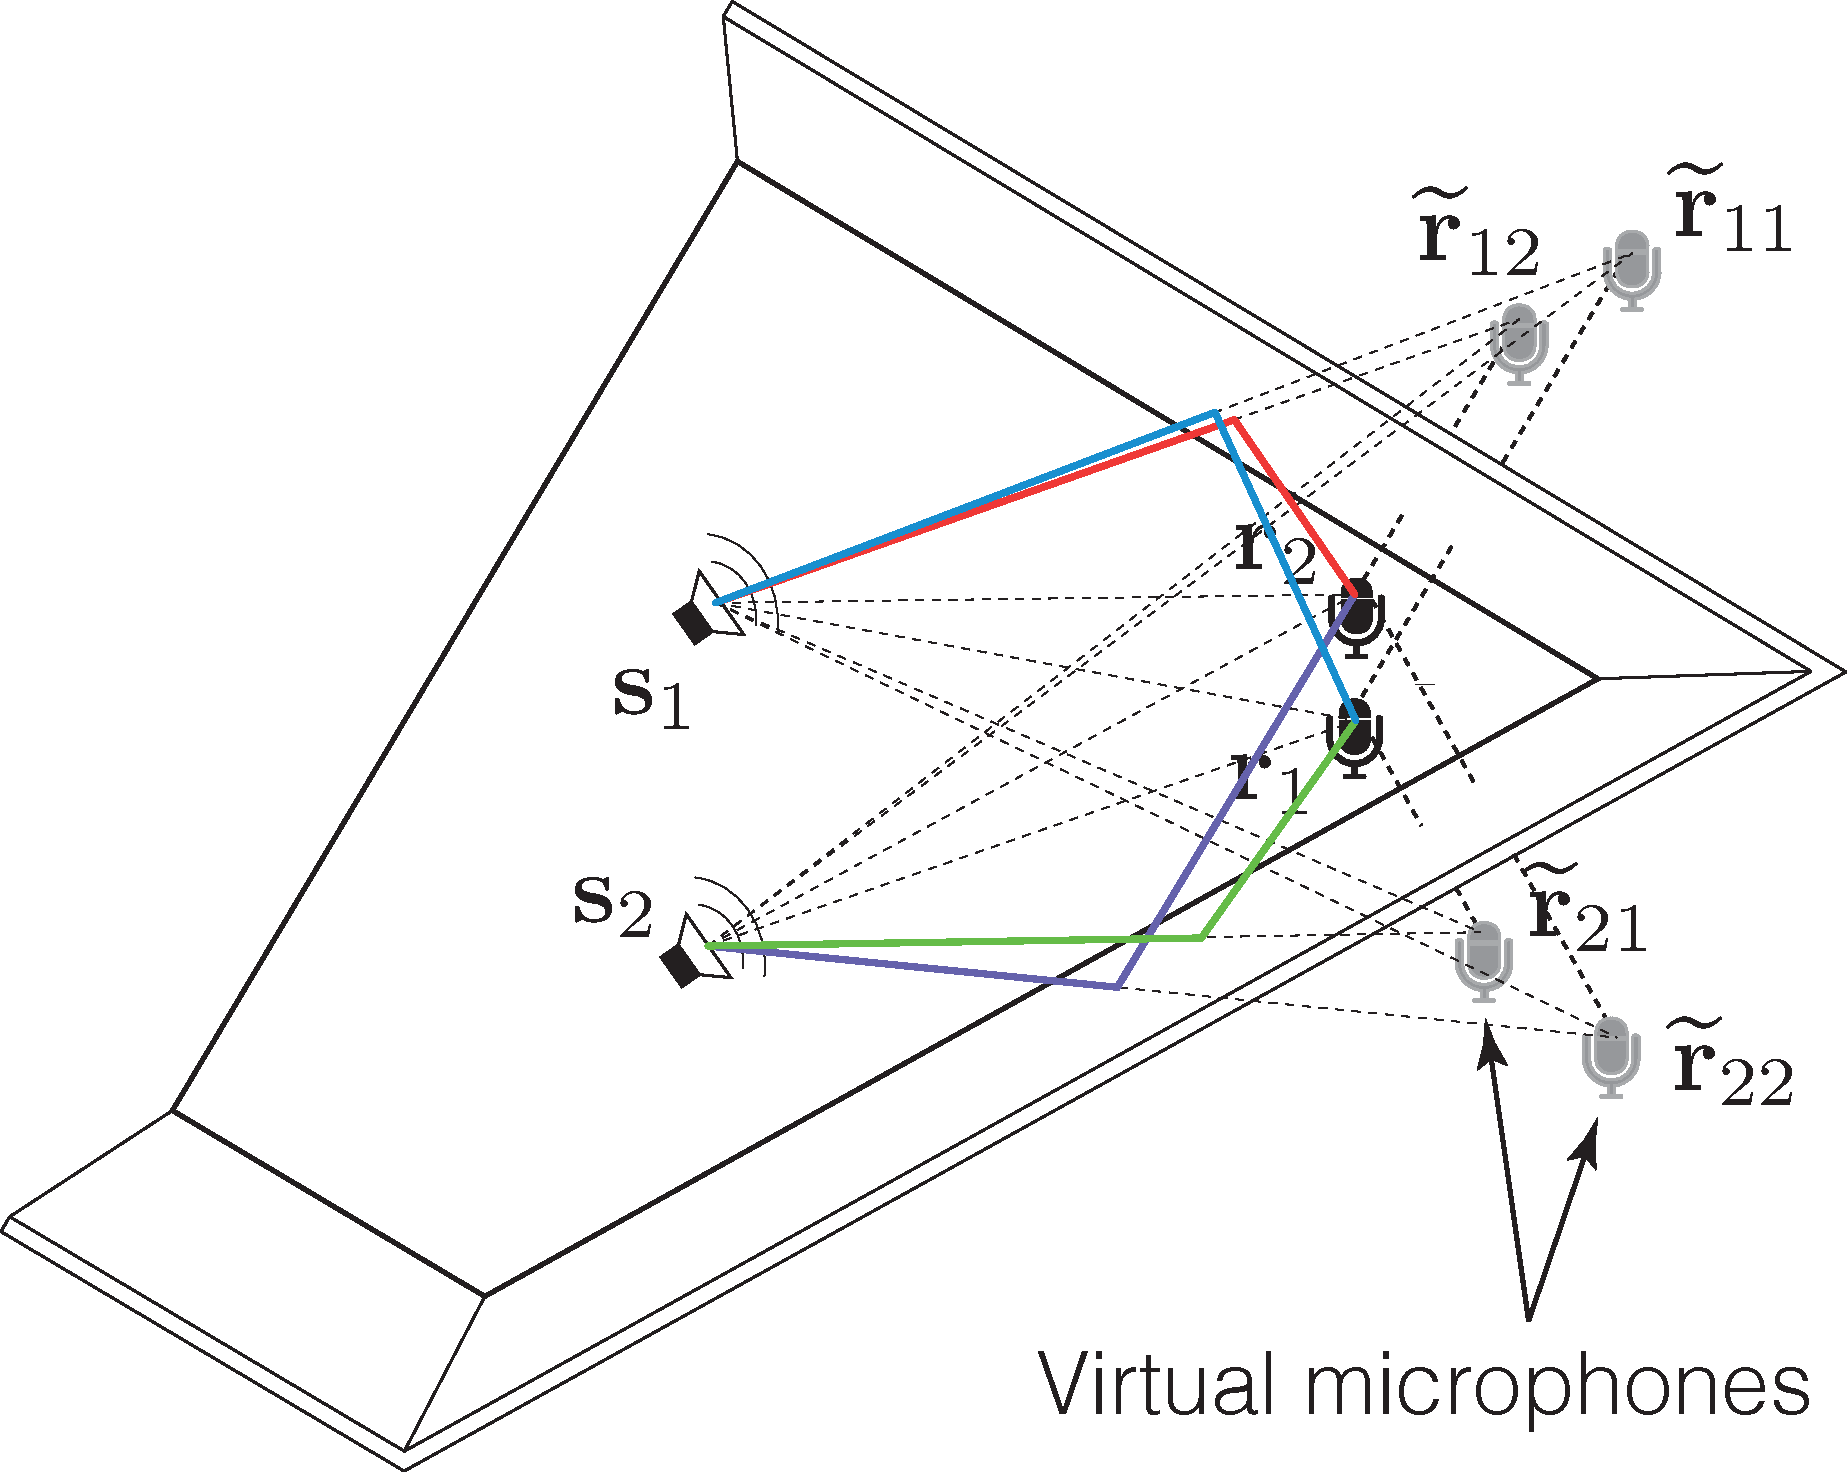
\includegraphics[width=.6\linewidth]{separake/separake.pdf}
    \end{sidecaption}
\end{figure}

\newthought{Traslating echoes into image arrays} provides an interesting geometrical interpretation in light of beamforming theory.
Real and virtual microphones form dipoles with diverse frequency-dependent directivity patterns.
By integrating more and more virtual microphones, the directivity patterns change and higher spatial selectivity can be achieved~\citeonly{dokmanic2015raking}.
This effect is shown in~\cref{fig:separake:directivity}.
Therefore, the goal of this work is to design audio source separation algorithms which benefit from this known spatial diversity.
\begin{figure}[b]
    \begin{fullwidth}
    \centering
    

\tikzset{every picture/.style={line width=0.75pt}} %set default line width to 0.75pt

\begin{tikzpicture}[x=0.75pt,y=0.75pt,yscale=-1,xscale=1]
%uncomment if require: \path (0,300); %set diagram left start at 0, and has height of 300

%Image [id:dp3129430507137261]
\draw (100,148) node  {\includegraphics[width=12pt]{acoustics/iconfinder_microphone_1608550.pdf}};
%Shape: Rectangle [id:dp30560892412693785]
\draw  [draw opacity=0][fill={rgb, 255:red, 255; green, 255; blue, 255 }  ,fill opacity=1 ] (30,40) -- (90,40) -- (90,100) -- (30,100) -- cycle ;
%Image [id:dp7096994311262355]
\draw (60,70) node  {
\includegraphics[width=45pt,height=45pt]{acoustics/iconfinder_ic_speaker_48px_352138.pdf}};

%Shape: Rectangle [id:dp4697494152917967]
\draw  [draw opacity=0][fill={rgb, 255:red, 155; green, 155; blue, 155 }  ,fill opacity=1 ] (120,20) -- (130,20) -- (130,180) -- (120,180) -- cycle ;
%Shape: Rectangle [id:dp004047242901594306]
\draw  [draw opacity=0][fill={rgb, 255:red, 155; green, 155; blue, 155 }  ,fill opacity=1 ] (30,170) -- (130,170) -- (130,180) -- (30,180) -- cycle ;
%Straight Lines [id:da07895276576528787]
\draw    (30,170) -- (120,170) -- (120,20) ;
%Image [id:dp41187969901424026]
\draw (150,148) node  {\includegraphics[width=12pt]{acoustics/iconfinder_microphone_1608550.pdf}};
%Image [id:dp5789764730979481]
\draw (460,148) node  {\includegraphics[width=12pt]{acoustics/iconfinder_microphone_1608550.pdf}};
%Shape: Rectangle [id:dp9000181446128821]
\draw  [draw opacity=0][fill={rgb, 255:red, 255; green, 255; blue, 255 }  ,fill opacity=1 ] (390,40) -- (450,40) -- (450,100) -- (390,100) -- cycle ;
%Image [id:dp2435207414441274]
\draw (420,70) node  {
\includegraphics[width=45pt,height=45pt]{acoustics/iconfinder_ic_speaker_48px_352138.pdf}};

%Shape: Rectangle [id:dp9398764926641255]
\draw  [draw opacity=0][fill={rgb, 255:red, 155; green, 155; blue, 155 }  ,fill opacity=1 ] (480,20) -- (490,20) -- (490,180) -- (480,180) -- cycle ;
%Shape: Rectangle [id:dp778971808734305]
\draw  [draw opacity=0][fill={rgb, 255:red, 155; green, 155; blue, 155 }  ,fill opacity=1 ] (390,170) -- (490,170) -- (490,180) -- (390,180) -- cycle ;
%Straight Lines [id:da3135305596380903]
\draw    (390,170) -- (480,170) -- (480,20) ;
%Image [id:dp7510496534085151]
\draw (510,148) node  {\includegraphics[width=12pt]{acoustics/iconfinder_microphone_1608550.pdf}};
%Image [id:dp46570823643682746]
\draw (460,198) node  {\includegraphics[width=12pt]{acoustics/iconfinder_microphone_1608550.pdf}};
%Shape: Rectangle [id:dp7037413163827391]
\draw  [draw opacity=0][fill={rgb, 255:red, 255; green, 255; blue, 255 }  ,fill opacity=0.69 ] (140,130) -- (160,130) -- (160,160) -- (140,160) -- cycle ;
%Shape: Rectangle [id:dp9860539015068507]
\draw  [draw opacity=0][fill={rgb, 255:red, 255; green, 255; blue, 255 }  ,fill opacity=0.69 ] (500,130) -- (520,130) -- (520,160) -- (500,160) -- cycle ;
%Shape: Rectangle [id:dp6314384514574135]
\draw  [draw opacity=0][fill={rgb, 255:red, 255; green, 255; blue, 255 }  ,fill opacity=0.69 ] (450,180) -- (470,180) -- (470,210) -- (450,210) -- cycle ;
%Image [id:dp35657556948669544]
\draw (250,100) node  {\includegraphics[width=120pt,height=120pt]{separake/rir_dipoles.pdf}};
%Image [id:dp09548352613616551]
\draw (610,100) node  {\includegraphics[width=120pt,height=120pt]{separake/rir_tripoles.pdf}};

% Text Node
\draw (105,212.5) node [anchor=north west][inner sep=0.75pt]  [font=\footnotesize] [align=left] {Virtual Dipoles};
% Text Node
\draw (472,212.5) node [anchor=north west][inner sep=0.75pt]  [font=\footnotesize] [align=left] {Virtual Tripoles};

\end{tikzpicture}

    \label{fig:separake:directivity}
    \caption{Frequency-dependent directivity pattern }
    \end{fullwidth}
\end{figure}

\section{Modeling}
Recalling the echo model for the \RIRs/, and assuming $\numEchs$ echoes per source are known, the approximate \RTFdef/ from source $\idxSrc$ to microphone $\idxMic$ writes
\begin{equation}
    \label{eq:separake:approx_tf}
    \tilde{H}_{\idxMicSrc}(f) = \sum_{\idxEch=0}^{\numEchs} \alpha_{\idxMicSrc}^{(\idxEch)} \cste^{-\csti 2 \pi f \tau_{\idxMicSrc}^{(\idxEch)}}.
\end{equation}
The far field assumption implies that only the relative arrival times are known, so we can arbitrarily fix the delay of the direct path to zero.
In addition, we assume all walls to be spectrally flat in the frequency range of interest and that $\alpha_{\idxMicSrc}^{(\idxEch)}$ are known up to a scaling (i.e. $\alpha_{\idxMicSrc}^{(0)} = 1$).
In this work the echoes properties are assumed to be known.

\mynewline
Assuming the narrowband approximation, the mixing process can be modeled model as in \cref{subsec:processing:model:stft}.
Therefore, the \STFTdef/ of the $\idxMic$-th microphone signal reads
\begin{equation}
    \label{eq:separake:stft}
    \MIC_\idxMic[k,l] = \sum_{\idxSrc = 1}^{\numSrcs} H_{\idxMicSrc}[k] \SRC_{\idxSrc}[k,l] + \NSE_\idxMic[k,l]
\end{equation}
with $k\in\klist{0,\ldots,F}$ and $l\in\klist{0,\ldots,T}$ being the frequency and frame index,
$H_{\idxMicSrc}[k]$ is the \DFT/ approximating the \RTF/ of~\eqref{eq:separake:approx_tf},
$\MIC_{\idxSrc}[k,l]$ the \STFT/ of the $\idxSrc$-th source signal, and $\NSE_\idxMic[k,l]$ a term including noise and model mismatch.
It is convenient to group the microphone observations in vector-matrix form,
\begin{equation}
    \MICS[k,l] = \FLTSS[k]\SRCS[k,l] + \NSES[k,l]
    ,
\end{equation}
where $\MICS[k,l],  \NSES[k,l] \in \bbC^{\numMics \times 1}$, $\SRCS[k,l] \in \bbC^{\numSrcs \times 1}$ and $\FLTSS[k,l] \in \bbC^{\numMics \times \numSrcs}$.

\mynewline
Let the squared magnitude of the spectrogram of the $\idxSrc$-th source be $\mP_\idxSrc = \klist{\powerOf{\SRC_\idxSrc}}_{kl} \in \bbR^{F\times T}$.
As depicted in~\cref{fig:separake:nmf_source}, the spectrogram can be modeled as the product of 2 non-negative matrices:
\marginpar{
    \centering
    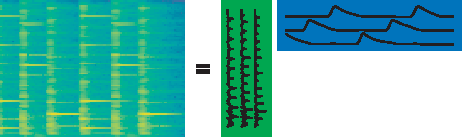
\includegraphics[width=\linewidth]{separake/nmf_example_source.pdf}
    \captionof{figure}{
        Spectrogram of a sound source signal decomposed into dictionary and activation
    }\label{fig:separake:nmf_source}
}
\begin{equation}
    \label{eq:separake:nmf}
    \mP_\idxSrc =  \mD_\idxSrc \mZ_\idxSrc,
\end{equation}
where $\mD_\idxSrc$ is the non-negative \textit{dictionary} whose contains the spectral can be interpreted as spectral templates of the source,
and the latent variables $\mZ_\idxSrc$, called \textit{activations}, indicates when and how this templates are activated.

\newthought{The NMF-based Audio Source Separation} can then be cast as an inference problem in which we maximize the likelihood of the observed $\MICS$ over all possible non-negative factorizations \eqref{eq:separake:nmf}.
This normally involves learning the channels, namely the frequency-domain mixing matrices $\FLTSS$.
Instead of learning them, we build the channels based on the prior knowledge of the earliest few echoes.

\section{Source Separation by NMF}
In this work we consider the two standard, well-understood multi-channel source separation algorithms which, by default, estimate the channels together with sources' dictionaries and activations.
The first algorithm is the \NMFdef/ via \MUdef/ and consider only the magnitudes of the transfer functions.
The second one is the multichannel \NMF/ via \EMdef/, which instead explicitly model the phases of the mixing filters.
In this work, we considered only the (over)determined case ($\numSrcs \leq \numMics$).
In the following we briefly describe the idea behind the two algorithms.
We reminds to the work of~\citeonly{ozerov2010multichannel} for further details.

\subsection{NMF using Multiplicative Updates (MU-NMF)}\label{sec:separake:mu}
\MU/ for \NMF/ only involve the magnitudes only and the updates rules are guaranteed non-negative as long as the initialization is.
This model have been originally proposed by in \citeonly{Lee:2001ti}, however we will consider its formulation as it appear in~\citeonly{ozerov2010multichannel}.
The observed multi-channel squared magnitude spectra $\mV_\idxMic = \klist{\powerOf{\MIC_\idxMic[k,l]}}_{kl}$ and their non-negative factorizations,
\begin{equation}
    \label{eq:mu_nmf}
    \wh{\mV}_\idxMic = \sum_{\idxSrc=1}^{\numSrcs} \diag(\vQ_{\idxMicSrc}) \mD_\idxSrc \mZ_\idxSrc , \quad \idxMic=1,\ldots,\numMics
\end{equation}
\marginpar{
    \centering
    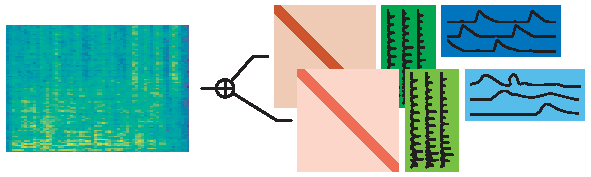
\includegraphics[width=\linewidth]{separake/mu_nmf_signal_model.pdf}
    \captionof{figure}{
        Schematics of the signal model used for \MU/-\NMF/.
    }\label{fig:separake:nmf_mu}
}
where $\vQ_{\idxMicSrc} = \klist{\powerOf{\FLT_{\idxMicSrc}[k]}}_k$ is the vector of squared magnitudes of the approximate \RTF/ between microphone $\idxMic$ and source $\idxSrc$.

\newthought{The MU cost function} is minimize the \textit{Itakura-Saito divergence} \citeonly{Fevotte:2011af} between the observed spectrogram $(\mV_{\idxMic}[k,l]$ and the model $\wh{\mV}_{\idxMic}[k,l]$, that is,
\begin{equation}
    \scrC_{\mathtt{MU}}(\Theta_{\mathtt{MU}}) = \sum_{\idxSrc k l} \calD_{\mathtt{IS}}(\mV_{\idxMic}[k,l] | \wh{\mV}_{\idxMic}[k,l])
    + \gamma \sum_\idxSrc \kvvbar{\mZ_\idxSrc}_1,
\end{equation}
where $\calD_{\mathtt{IS}}( v | \hat{v} ) = \frac{v}{\hat{v}} - \log \frac{v}{\hat{v}} - 1$ and $\Theta_{\mathtt{MU}} = \{\vQ_{\idxMicSrc}, \set{\mD_\idxSrc, \mZ_\idxSrc}_\idxSrc\}_{\idxMicSrc}$ is the set of parameters.
We add an $\ell_1$-penalty term to promote sparsity in the activations due to the potentially large size of the dictionary~\citeonly{Sun:2013co}.

\newthought{The MU updating rules} for each scalar parameter of interest $\theta$ are obtained by multiplying its value at previous iteration by the ratio of the negative and positive parts of the derivative of the criterion \wrt/ this parameter, namely,
\begin{equation*}
    \theta \gets \theta \frac{\kbracket{\knabla_\theta \scrC_{\mathtt{MU}}(\Theta_{\mathtt{MU}})}_{-}}
                             {\kbracket{\knabla_\theta \scrC_{\mathtt{MU}}(\Theta_{\mathtt{MU}})}_{+}}
\end{equation*}
where $\scrC_{\mathtt{MU}}(\Theta_{\mathtt{MU}}) = {\kbracket{\knabla_\theta \scrC_{\mathtt{MU}}(\Theta_{\mathtt{MU}})}_{+}} - {\kbracket{\knabla_\theta \scrC_{\mathtt{MU}}(\Theta_{\mathtt{MU}})}_{-}}$ and the summands are both nonnegative.
By adapting the original \MU/ rule derivations from \citeauthor{ozerov2010multichannel}, we obtain:
\begin{align}
    \vQ_{\idxMicSrc} &\gets\vQ_{\idxMicSrc} \odot \frac{\kbracket{\wh{\mV}_\idxSrc^{-2} \odot \mV_\idxSrc \odot \kparen{\mZ_\idxSrc \mD_\idxSrc}}\onesVect_{1\times T}}{
                                            \kbracket{\wh{\mV}_\idxSrc^{-1} \odot \kparen{\mZ_\idxSrc \mD_\idxSrc}}\onesVect_{1\times T}}\\
    \mZ_\idxSrc &\gets \mZ_\idxSrc \odot \frac{\sum_\idxMic \ktranspose{(\diag(\vQ_{\idxMicSrc}) \mD_\idxSrc)} \kparen{\mV_\idxSrc \odot \wh{\mV}_\idxSrc^{-2}}}{
                                            \sum_\idxMic \ktranspose{(\diag(\vQ_{\idxMicSrc}) \mD_\idxSrc)} \wh{\mV}_\idxSrc^{-1} + \gamma},\\
    \mD_\idxSrc &\gets \mD_\idxSrc \odot \frac{\sum_\idxMic \ktranspose{ \diag(\vQ_{\idxMicSrc})} \kparen{\mV_\idxSrc \odot \wh{\mV}_\idxSrc^{-2}}\ktranspose{\mZ_\idxSrc}}{
                                            \sum_\idxMic \ktranspose{ \diag(\vQ_{\idxMicSrc})} \wh{\mV}_\idxSrc^{-1} \ktranspose{\mZ_\idxSrc}},
\end{align}
where multiplication $\odot$, power, and division are element-wise and $\onesVect_{1\times T}$ is a $N$-vector of ones,.

\subsection{NMF using Expectation Maximization (EM-NMF)}\label{sec:separake:em}
Unlike the \MU/ algorithm that independently maximizes the log-likelihood of spectral magnitudes, the \EM/-\NMF/ maximizes the joint log-likelihood over all complex-valued channels~\citeonly{ozerov2010multichannel}.
Hence, the model takes explicitly into account observed phases.
In this approach, each source $\idxSrc$ is modeled as complex Gaussian in the form of
\begin{equation}
    \SRC_\idxSrc[k,l] \sim \mathcal{N}_c \kparen{0, (\mD_\idxSrc\mZ_\idxSrc)_{kl}},
\end{equation}
and the magnitude spectrum $\mP_\idxSrc$ of \eqref{eq:separake:nmf} can be understood as the variance of source $\idxSrc$.
\\Under this model, and assuming uncorrelated noise, the microphone signals also follow a complex Gaussian distribution with covariance matrix
\begin{equation}
    \mSigma_{\MICS}[k,l] = \FLTSS[k] \mSigma_{\SRCS} [k,l] \khermitian{\FLTSS}[k] + \mSigma_{\NSES}[k,l]
    ,
\end{equation}
where $\mSigma_{\SRCS}$ and $\mSigma_{\NSES}$ are the covariance matrix of the sources and noise, respectively.

\newthought{The EM cost function} correspond to the negative log-likelihood of the observed signal, that is,
\begin{equation}\label{eq:separake:loglike}
    \scrC_{\mathtt{EM}}(\Theta_{\mathtt{EM}}) = \sum\limits_{kl} \trace\kparen{\MICS[k,l] \khermitian{\MICS[k,l]} \mSigma_{\MICS}^{-1}[k,l]} \\
    + \log\det\mSigma_{\MICS}[k,l].
\end{equation}
where the $\Theta_{\mathtt{EM}} = \set{\FLTSS, \set{\mD_\idxSrc, \mZ_\idxSrc}_\idxSrc, \mSigma_{\NSES}}$ is the set of parameters.

\newthought{The EM algorithm} estimates all the parameters $\Theta$ by alternating between the so-called E-step and M-step.
In a nutshell, one iteration the E-step consists of computing the \textit{conditional expectation} of the the log likelihood of $\scrC_{\mathtt{EM}}$ with respect to the current parameter estimates,
and the M-step re-estimating the parameters by maximizing the conditional expectation of the log-likelihood of $\scrC_{\mathtt{EM}}$.
This quantity can be efficiently minimized using the \EM/ algorithm proposed in~\citeonly{ozerov2010multichannel}.
Moreover, since adding sparsity priors is not straightforward in the \EM/ framework, it was left for future work.
% \begin{description}
%     \item[E-step:] Conditional expectation \wrt/ the current parameters
%     \begin{align}
%         a &= a\\
%         a &= a\\
%     \end{align}
%     \item[M-step:] Updates of the parameters
%     \begin{align}
%         \mD = \frac{1}{N} \sum_N
%     \end{align}
% \end{description}

% \subsection{Reconstruction of the sources}
% The reconstruction of the image sources is achieved by Wiener filtering, namely
% \begin{equation}
%     \IMG_\idxMicSrc[k,l] = \FLT_{\idxMicSrc}[k] \SRC_\idxSrc[k,l] =
% \end{equation}

\section{Echo-aware Source Separation}
To evaluate the usefulness of echoes in source separation, we modified the the multi-channel \NMF/ framework of \citeauthor{ozerov2010multichannel}~\citeonly{ozerov2010multichannel}.
The knowledge of the echoes in embedded in the embedded in the model by approximating the entries of mixing matrix with~\eqref{eq:approx_tf}, that is,
\begin{equation}
    \begin{aligned}
        \FLT_{\idxMicSrc}[k] &= \sum_{\idxEch=0}^{\numEchs} \alpha_{\idxMicSrc}^{(\idxEch)} \cste^{-\csti 2 \pi f_k \tau_{\idxMicSrc}^{(\idxEch)}},\\
        \FLTSS[k] &= \kbracket{\FLT_{\idxMicSrc}[k]}_{\idxMicSrc},
    \end{aligned}
\end{equation}
where $f_k = k\Fs/F$ are the discretized frequencies in Hz corresponding to the $k$-th bin in the \DFT/.
\\Futhermore, the early-echo channel model is kept fixed throughout the iterations.
Moreover, instead of updating both sources' dictionaries and activations, we adapted pre-trained dictionaries to better guide the source separation.

\newthought{Pre-trained Dictionaries} are a typical way to inform the \NMF/ algorithm, and sometimes referred to as \textit{supervised \NMF/}.
The idea is run \NMF/-based source separation on a set of training and collect the atoms of the estimated non-negative matrices\citeonly{schmidt2006single}.
At the test phase, this atoms are used as basis vectors for the dictionary matrix (\ie/, $\mD$) and can be used as a good initialization point or kept fixed in the algorithm\sidenote{
    In the context of \NMF/-based music transcription applied to piano music, the dictionary can be the collection of spectral templates, each of which is associated to a piano notes~\citeonly{muller2015fundamentals}}.
This can be seen as an instance of the problem of \textit{dictionary learning} which exist also in many other research field.
For audio source separation, this ideas has been studied extensively since promising results were obtained, even in single channel scenarios ~\citeonly{smaragdis2009sparse}.
Ad discussed later in~\cref{subsec:separake:dictionary}, in this work we will use two different dictionaries: one \textit{universal}, and the other \textit{speaker-specific}.

\newthought{Neglecting the reverberation} (or working in the anechoic regime) leads to a constant $\vQ_{\idxMicSrc}$ for all $\idxSrc$ and $\idxMic$.
A consequence is that the \MU/-\NMF/ framework breaks down with a universal dictionary, namely, $\mD = \mD_j\;\forall j$.
Indeed, \eqref{eq:mu_nmf} becomes the same for all $\idxMic$,
\begin{equation*}
    \wh{\mV}_\idxMic = \sum_{\idxSrc} \mD \mZ_\idxSrc = \mD \sum_\idxSrc \mZ_\idxSrc,
\end{equation*}
so even with the correct atoms identified, we can assign them to any source without changing the value of the cost function.
Therefore, anechoic multi-channel separation with a universal dictionary cannot work well.
This intuitive reasoning is corroborated by numerical experiments in Section \ref{sec:results}.
The problem is overcome by the \EM/-\NMF/ algorithm which keeps the channel phase and is thus able to exploit the phase diversity across the array.
Of course, as showed in this work, it is also overcome by using echoes.

\section{Numerical Experiments}

We test our hypotheses through computer simulations.
In the following, we describe the simulation setup, dictionary learning protocols, and we discuss the results.

\subsection{Setup}
An array of three microphones arranged on the corners of an equilateral triangle with edge length $\SI{0.3}{\m}$ is placed in the corner of a 3D room with 7 walls.
We select 40 sources at random locations at a distance ranging from $\SI{2.5}{\m}$ to $\SI{4}{\m}$ from the microphone array.
Pairs of sources are chosen so that they are at least $\SI{1}{\m}$ apart.
The floor plan and the locations of microphones are depicted in Figure~\ref{fig:separake:rir_room}\marginpar{
    \centering
    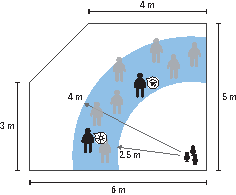
\includegraphics[width=\linewidth]{figures/separake/room_setup}
    \captionof{figure}{
        The simulated scenario.
    }
    \label{fig:separake:rir_room}
}.
The scenario is repeated for every two active sources out of the 780 possible pairs.

\mynewline
The sound propagation between sources and microphones is simulated using the
image source model implemented in \library{pyroomacoustics} Python package~\citeonly{scheibler2017pyroomacoustics}.
The wall absorption factor is set to $0.4$, leading to a $\RT$ of approximately $\SI{100}{\ms}$.
The sampling frequency is set to $\SI{16}{\kHz}$, \STFT/ frame size to $2048$ samples with $50\%$ overlap between frames, and we use a cosine window for analysis and synthesis.
Partial \RTFs/ are then built from the $\numEchs$ nearest image microphones.
The global delay is discarded, and only the relative amplitudes between echoes are kept.

\mynewline
With this setup, we perform three different experiments.
In the first one, we evaluate \MU/-\NMF/ with a universal dictionary.
In the other two, we evaluate the performance of \MU/-\NMF/ and \EM/-\NMF/ with speaker-specific dictionaries.
We vary $\numEchs$ from 1 to 6 and use three baseline scenarios:
\begin{enumerate}
\item \textit{anechoic}: Anechoic conditions, no model mismatch.
\item \textit{learn}: The \RTFs/ are learned from the data along the activations as originally proposed~\citeonly{ozerov2010multichannel}.
\item \textit{no echoes}: Reverberation is present but ignored (i.e. $\numEchs=0$).
\end{enumerate}
With the universal dictionary, the large number of latent variables warrants the introduction of sparsity-inducing regularization.
The value of the regularization parameter $\gamma$ was chosen by a grid search on a holdout set with the signal-to-distortion ratio ($\SDR$) as the figure of merit \citeonly{vincent2007first} (See ~\cref{tab:separake:gamma}).

\begin{table}
    \begin{sidecaption}[]{
        Value of the regularization parameter $\gamma$ used with the universal dictionary.
        }[tab:separake:gamma]
        \centering
        \small
        \begin{tabular*}{\linewidth}{@{\extracolsep{\fill}}lccccccccc@{}}
    \toprule
     &       &          & \multicolumn{7}{c}{{\footnotesize Number of echoes $\numEchs$}} \\
     \cmidrule{4-10}
     & anechoic & learn & 0 & 1 & 2 & 3 & 4 & 5 & 6 \\
     \cmidrule{2-10}
     $\gamma = $ & $10$ & $10^{-1}$ & $10$ & $10^{-3}$ & 0 & 0 & 0 & 0 & 0 \\
     \bottomrule
\end{tabular*}
    \end{sidecaption}
\end{table}


\subsection{Dictionary Training, Test Set}\label{subsec:separake:dictionary}
First, we introduce a dictionary learned from available training data.
We explore both speaker-specific and universal dictionaries \citeonly{Sun:2013co}.
Speaker-specific dictionaries can be beneficial when speakers are known in advance.
Universal dictionary is more versatile but gives a weaker regularization prior.

\begin{figure}[h]
    \begin{fullwidth}
    \centering
    \subfloat[mu_univ][Universal dictionary]{
        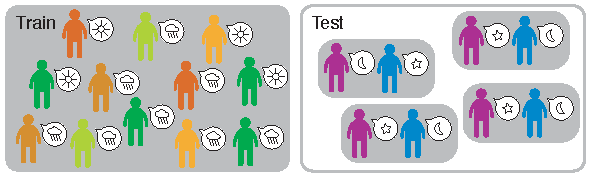
\includegraphics[width=0.48\linewidth]{separake/dict_universal.pdf}
        \label{fig:separake:dict_univ}}
    \hfill
    \subfloat[mu_spkr][Speaker-specific dictionary]{
        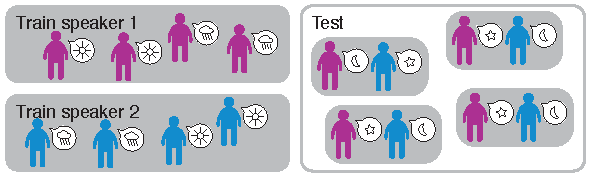
\includegraphics[width=0.48\linewidth]{separake/dict_speaker_dep.pdf}
        \label{fig:separake:dict_spk}}
    \label{fig:separake:results}
    \end{fullwidth}
\end{figure}


\newthought{Universal Dictionary:} Following the methodology of \citeonly{Sun:2013co} we select 25 male and 25 female speakers
and use all available training sentences to form the universal dictionary
$
    \mD = [\mD_1^\mathtt{M}\cdots \mD_{25}^\mathtt{M}\,\mD_{1}^\mathtt{F}\cdots\mD_{25}^\mathtt{F}].
$
The test signals were selected from speakers \emph{and} utterances outside the training set.
The number of latent variables per speaker is 10 so that with STFT frame size of 2048 we have $\mD\in\R^{1025\times500}$.

\newthought{Speaker-Specific Dictionary:}
Two dictionaries were trained on one male and one female speaker.
One utterance per speaker was excluded to be used for testing.
The number of latent variables per speaker was set to $20$.

\mynewline
All dictionaries were trained on samples from the TIMIT corpus \citeonly{garofolo1993timit} using the \NMF/ solver in \library{scikit-learn} Python package~\citeonly{pedregosa2011scikit}.

\subsection{Implementation:}
Authors of \citeonly{ozerov2010multichannel} provide a Matlab implementation\sidenote{
    \href{http://www.irisa.fr/metiss/ozerov/Software/multi_nmf_toolbox.zip}{Multichannel nonnegative matrix factorization toolbox (in Matlab)}
} of \MU/-\NMF/ and \EM/-\NMF/ methods for stereo separation.
We ported their code to Python and extended it to arbitrary number of input channels\sidenote{
    Our implementation and all experimental code are publicly available in line with the philosophy of reproducible research.
}.
However this software features some ad-hoc decisions which do not fit our scenario.
Thus, we provide a Python3 adaptation with the following modifications.
\begin{itemize}
    \item First the original code was restricted to the 2-channel case, i.e.  $\numMics = 2$.
    Thus, in order to embrace the specifics of our scenario and for sake of generalization, we extend it to the multi-channel case, that is $\forall \numMics \geq 1$.
    \item the \MU/-\NMF/ was modified to handle sparsity constraint as described in \ref{sec:separake:mu}.
    \item since \EM/ method degenerates where zero-valued entries are present in the dictionary matrix, $\mD$, all these entries are initially set to a small constant value of $10^{-6}$.
    \item the code was further modified to deal with fixed dictionary and channel models matrices, which are normalized in order to avoid indeterminacy issues \citeonly{ozerov2010multichannel}.
\end{itemize}
Now to conclude with, no \textit{simulated annealing} strategies are not used in the final experiments.
In fact in some preliminary and informal investigations we noticed that this yields to better results then using annealing.
In the experiments, the number of iterations for \MU/-\NMF/ (\EM/-\NMF/) was set to $200$ ($300$).

\subsection{Results}
\label{sec:results}

We evaluate the performance in terms of signal-to-distortion ratio (\SDR) and source-to-interference ratio (\SIR) as defined in \citeonly{vincent2007first}.
We compute these metrics using the \library{mir\_eval} toolbox~\citeonly{raffel2014mir_eval}.

\mynewline
The distributions of \SDR{} and \SIR{} for separation using \MU/-\NMF/ and a universal dictionary are shown in \cref{fig:separake:mu_univ}, with a summary in \cref{fig:separake:median}.
We use the median performance to compare the results from different algorithms.
First, we confirm that separation fails for flat \RTFs/ (\textit{anechoic} and $\numEchs=0$) with \SIR{} at around 0~dB.
Learning the \RTFs/ performs somewhat better in terms of \SIR{} than in terms of \SDR{}, though both are low.
Introducing approximate \RTFs/ dramatically improves performance: the proposed approach outperforms the learned approach even with a single echo.
With up to six echoes, gains are +2~dB \SDR{} and +5~dB \SIR{}.
Interestingly, with more than one echo, non-negativity and echo priors already sufficient for achieving good separation, overlooking the $\ell_1$ regularization.


\begin{figure}[t]
    \begin{fullwidth}
    \centering
    \subfloat[mu_univ][MU-NMF, Universal dictionary]{
        \includegraphics[width=0.32\linewidth]{separake/20171025-111558_5ae4058906_near_wall_mu_UnivDict_violin_plot.pdf}
        \label{fig:separake:mu_univ}}
    \hfill
    \subfloat[mu_spkr][MU-NMF, Speaker-specific dictionary]{
        \includegraphics[width=0.32\linewidth]{separake/20171026-192746_360771b8ce_near_wall_mu_SpkrDict_violin_plot.pdf}
        \label{fig:separake:mu_spkr}}
    \hfill
    \subfloat[em_spkr][EM-NMF, Speaker-specific dictionary]{
        \includegraphics[width=0.32\linewidth]{separake/20171027-050909_e9d8c07aef6_near_wall_em_SpkrDict_violin_plot.pdf}
        \label{fig:separake:em_spkr}}
    \caption{Distribution of SDR and SIR for male and female speakers as a function of the number of echoes included in modeling, and comparison with the three baselines.}
    \label{fig:separake:results}
    \end{fullwidth}
\end{figure}


\begin{figure}[b]
    \begin{sidecaption}[]{
            Summary of the median SDR and SIR for the different algorithms evaluated.
            \label{fig:separake:median}
        }[fig:separake:median]
        \centering
        \small
        \includegraphics[width=\linewidth]{separake/all_medians.pdf}
    \end{sidecaption}
\end{figure}


\mynewline
Separation with speaker-dependent dictionaries is less challenging since we have a stronger prior.
Accordingly, as shown in ~\cref{fig:separake:mu_spkr,fig:separake:median}, \MU/-\NMF/ now achieves a certain degree of separation even without the channel information.
The gains from using echoes are smaller, though one echo is still sufficient to match the median performance of learned \RTFs/.
Using an echo, however, results in a smaller variance, while adding more echoes further improves \SDR{} (\SIR) by up to +2~dB (+3~dB).

\mynewline
In the same scenario, \EM/-\NMF/ (\cref{fig:separake:em_spkr}) has near-perfect performance on anechoic signals which is expected as the problem is overdetermined.
For \MU/, a single echo suffices to reach the performance of learned \RTFs/ and further improve it.
Moreover, echoes significantly improve separation quality as illustrated by up to 3~dB improvement over \textit{learn}.
It is interesting to note that in all experiments the first three echoes near-saturate the metrics.
This is good news since higher order echoes are hard to estimate.

% \begin{itemize}
%    \item Universal dictionary scenario: Here, the speakers are unknown.
%    \begin{itemize}
%        \item Because the MU method does not use phase and hence no time delay information across channels, source separation in the anechoic scenario is impossible.
%              Here, we see that using reverberated signals instead with knowledge of only a few echoes significantly improve source separation performance: up to +2dB SDR and +5 dB SIR.
%        \item Using a fixed echo model for channels also outperform learning the channels, even with a single echo.
%        \item Note that EM could not be used for the universal dictionary scenario, because the corresponding model is not designed to handle dictionaries with hundreds of atoms. A sparsity-enforcing Bayesian prior on the estimated activation Z would need to be included, which is not straightforward.
%        \item Increasing the number of known echoes beyond 3 does not bring significant improvement.
%    \end{itemize}
%    \item Speaker-dependent dictionary scenario. This scenario is on the one hand easier because speakers are known and on the other hand harder because much less training data is used, allowing much fewer atoms to represent speech in the dictionaries.
%    \begin{itemize}
%        \item Unsurprisingly, EM performs extremely well in the anechoic setting. This is because perfect knowledge of the complex-valued over-determined mixing filters is then available, through the time differences of arrival. Results would likely be very different in an under-determined setting, where perfect filter knowledge is not enough to separate signals.
%        \item Once again, it is showed that using knowledge of a few echoes significantly improve results with respect to an anechoic model, up to +2dB SDR and +3dB SIR for both methods.
%        \item EM performs slightly better (+1.5 dB) than MU in terms of SIR, suggesting that modeling the phase of mixing filters help.
%        \item In this scenario, knowledge of the echoes starts significantly outperforming the baseline (the learned model) when 3 echoes are known (+3dB SIR).
%        \item Again, increasing the number of known echoes beyond 3 does not bring significant improvement.
%    \end{itemize}
% \end{itemize}

\section{Conclusion}
In this work, we investigated the role of early echoes for the problem of sound source separation.
Unlike earlier work, instead of fitting echo model or trying to estimate the blindly the acoustic channels,
we investigate the potential of including the properties of known echoes in well established \NMF/-based source separation algorithms.
In particulars, we modified the \MU/ approach --- which consider only spectral magnitudes--- and the \EM/ --- which accounts for complex spectra ---
by integrating a simple echo model.
Despite its simplicity, such echo model lend itself to a interesting interpretation by revising the \ISM/ model:
to each echo corresponds an image microphones (instead of image source as in \ISM/).
It follows that real and image microphone can be considered as microphones arrays with specific directivity pattern.
\\Numerical results shows that echoes seem to play an essential role in magnitude-only algorithms, like the \MU/-\NMF/.
In general, the showed that using knowledge of a few echoes significantly improve results with respect to an anechoic model.
This improvement is measured by the standard metrics even when compared to approaches that learn the transfer functions.
To conclude with, does echoes helps sound source separation? The answer is \textit{yes}.

\newthought{Future work} on echo-aware source separation includes:
\begin{itemize}
    \item integrating the blind estimation of the echoes properties, \eg/ using the proposed algorithm \blaster{}.
    \item including the late reverberation part in the mixing matrices;
    \item experiments with more microphone, room configurations, more source on real data, \eg/ using the one offered by the \dEchorate{} dataset.
\end{itemize}

\chapter{Sound Source Localization \& \library{Mirage}}\label{chap:mirage}

\marginpar{%
    \footnotesize
    \textbf{Keywords:} Sound Source Localization, Image Microphones, Acoustic Echoes, TDOA Estimation.
    \\\textbf{Resources:}
    \begin{itemize}
        \item \href{https://ieeexplore.ieee.org/document/8683534}{Paper}
        \item \href{https://github.com/Chutlhu/mirage}{Code}
        \item \href{https://sigport.org/documents/mirage-2d-sound-source-localization-using-microphone-pair-augmentation-echoes}{Poster}
    \end{itemize}
}

\newthought{Synopsis} \synopsisChMirage

\mynewline
Together with~\cref{ch:lantern}, this chapter describes methods and results published in~\cite{di2019mirage}, which considers only stereophonic recordings.
In this sense, this chapter provides an application of the~\cref{ch:lantern}.
Subsequently, the proposed approach was to multi-microphone recordings in collaboration with Randy Gomez from Honda Research Institute.


% \subsection{Literature review: an acoustic perspective}
% Bibliography with respect to sound propagation

% \subsection{Literature review an algorithmic perspective}
% Bibliography with respect to learning and knowledge approaches

% \newthoughtpar{Knowledge-based vs. learning-based approaches}

% \newthoughtpar{Regression vs. classification approaches}

% \section{Background in SSL}
% \begin{itemize}
%     \item 1D SSL: AOA estimation
%     \item 2D SSL: azimuth and elevation estimation
%     \item 3D SSL: polar and cartesian coordinates
% \end{itemize}

% \subsection{Stereophonic SSL and 1D SSL}

% \newthoughtpar{Binaural SSL}

% \subsection{Multichannel SSL and 2D SSL}

% \section{\mirage: microphone augmentation with echoes}

% \section{Experimental evaluation}

% --- Margin Figure
\section{Literature review in Echo-aware Sound Source Localization}
Common to most sound source localization approaches reviewed in ~\cref{subsec:application:localization} is the challenge posed by environment reverberation.
It is typical to observe that \ac{DOAs} estimation degrades with increasing acoustic reflection~\citeonly{chen2006time}.
For these reasons, most sound source localization methods regard reverberation and, in particular, acoustic echoes as a nuisance.
Room reverberation is considered in the works~\citeonly{rui2004time, chen2006time, zhang2007maximum} while the authors of~\citeonly{weinstein1994iterative, taghizadeh2015spatial, salvati2016sound} attempt to solve \SSL/ by estimating the full \RIRs/.
However, both the cases have drawbacks: in the former, the generic model for reverberation does not reduce strong early echoes, and in the latter, \RIRs/ estimation is a difficult task.

\mynewline
The echo-aware sound source localization methods take another direction: they exploit the closed-form relation between echoes timings and audio scene geometry expressed by the \ISMdef/.
Early works such as~\citeonly{korhonen2008acoustic, ribeiro2010turning, ribeiro2010using, svaizer2011use} uses knowledge form the room geometry to estimated the position of the sound source with respect to the arrays.
This idea was subsequently extended in later works, reducing the amount of prior knowledge required or addressing different applications.
The authors of \citeonly{nakashima2010localization}  study the \SSL/ problem in binaural recordings.
To improve localization, they propose to used ad-hoc reflectors as artificial \textit{pinnae} and a simple reflection model.
In the work~\citeonly{krekovic2016echoslam}, the author addresses the problem \ac{SLAM}\sidenote{
    \ac{SLAM} enables the estimation of a moving robot’s position in relation to a number of external acoustic sources.
} using echoes.
The authors of~\citeonly{an2018reflection} propose to use cameras, depth sensors, and laser sensors to identify reflectors and build a corresponding acoustic model that is used
for echo-aware \ac{SSL}.
Finally, in a very recent work, the well-known \ac{MUSIC} framework for localizing multiple sources is modified for accounting an echo model for the spherical harmonic representation~\citeonly{birnie2020reflection}

\mynewline
All the above mentioned echo-aware methods are explicitly knowledge-driven, namely, using closed-form solutions based on physics, acoustics, and signal processing models.
As explained in the previous chapter, data-driven methods, especially \ac{DNN}, have been successfully applied to address \SSL/.
The main benefit is in their ability to learn complex mapping functions based on simple input-output pairs.
However, they are typically trained for specific applications and use-cases (\eg/, arrays geometry, acoustic conditions, \etc/) and fail whenever test conditions strongly mismatch training conditions.

\section{Proposed Approach}
In the work \cite{di2019mirage} we proposed to combine the best of the two worlds:
using a deep learning model to estimate challenging acoustic parameters and a physically-motivated model to map such parameters to source's \DOAs/.
To this end, we introduce the framework of \MIRAGEdef/ for \SSL/, based on the \textit{image microphones} model~\citeonly{bergamo2004collaborative,korhonen2008acoustic} (See~\cref{sec:separake:sota}).

\mynewline
Let us consider a simple yet common scenario to illustrate this idea:
two microphones, one source, and a nearby reflective surface, as illustrated in Fig. \cref{fig:mirage:scene}.
\marginpar{%
    \centering
    \footnotesize
    \includegraphics[trim={50 70 50 150},clip,width=\linewidth]{mirage/scene.pdf}
    \captionof{figure}{%
        Typical setup with one source source recorded by two microphones.
        The illustration shows direct sound path (blue lines) and resulting first-order echoes (orange lines).}
    \label{fig:mirage:scene}
}
This may occur when the sensors are placed on a table or next to a wall. Striking examples of these scenarios are the smart table-top devices, such as Amazon Echo, Google Home, \etc/.
The reflective surface is assumed to be the most reflective and closest one to the microphones in the environment, generating the strongest and earliest echo in each microphone.
Under this \textit{close-surface} model, we ask the following question:
\begin{enumerate}
    \item Can early echoes be estimated from two-microphone recordings of an unknown source?
    \item Can early echoes be used to estimate both the azimuth and elevation angles of the source, an \textit{impossible} task in free field conditions?
\end{enumerate}

\newthought{The First Question} was already addressed in~\Cref{ch:lantern}.
In particular, we proposed to use a \ac{DNN} trained on a simulated close-surface dataset to estimate early echoes properties from audio features.

\newthought{To answer the Second Question}, we propose the \ac{MIRAGE} framework.
It exploits echoes' time of arrival by expressing them as \acp{TDOA} in the \textit{virtual 4-microphone array} formed by the true microphone pair and its image with respect to the reflective surface.
We show that this framework approximately estimates echo properties, perform similarly to a correlation-based method in azimuth estimation for the considered
scenario and estimates \textit{impossible} elevation angles with good accuracy in noiseless settings using two microphones only.


\section{Background in microphone array SSL}\label{sec:background}
In this section, we briefly review some necessary background in microphone array \ac{SSL}.
Let us assume a microphone array of $\idxMic$ sensors is placed inside a room and records the sound emitted by one static point sound source ($\numSrcs=1$).
In all generality, the relationship between the signal $\mic_\idxMic$ recorded by the $\idxMic$-th sensor placed at fixed position $\positionMicrophone_\idxMic$ and the signal $\src$ emitted by the source at fixed position $\positionSource$ is defined by:
\begin{equation}\label{eq:mirage:anymic_time}
\mic_i[n] = (\flt_\idxMic \convDis \src)[n]  \; + \; \nse_\idxMic[n],
\end{equation}
where the convolution with \RIR/ $\flt_\idxMic[n]$ embodies the fact that sensor $\idxMic$ receives a spatial image of the source and $\nse_\idxMic$ denotes possible measurement noise.
As fully described in~\cref{ch:acoustic}, the \RIR/ depends on the spatial parameters of the scene: microphone positions, source position \wrt/ the room, as well as the room acoustic properties (size, absorption, and diffuseness of the wall materials).

\mynewline
Let us assume that \RIRs/ follows the echo model under the narrowband approximation presented in~\cref{subsec:processing:stft}.
Therefore, in the discrete-frequency domain, this leads to
\begin{equation}\label{eq:mirage:rir}
    \FLT_\idxMic[k] = \sum_{\idxEch=0}^{\numEchs}  \; \alpha_\idxMic^{(\idxEch)}[k] \; \cste^{- \csti 2 \pi f_k \tau_\idxMic^{(\idxEch)}} \; + \; \varepsilon_\idxMic[k],
\end{equation}
where $f_k$ is the $k$-th frequency bin and the error term $\varepsilon_i[k]$ collects later echoes, the reverberation tail, diffusion, and noise.
A time-domain example of \RIR/ is shown in Fig.~\cref{fig:mirage:rirs} (left).
In this work, we will consider only the first strongest echo, therefore $R = 1$.
Note that $r=0$ denotes the ideal propagation path.

\begin{figure}[t]
    \begin{sidecaption}[RIRs within the MIRAGE framework]{%
        (Left) A typical simulated \RIR/ with annotated components.
        (Right) Superposition of two RIRs and visualization of time difference
        of arrival between direct paths (\ac{TDOA}), first echoes (\ac{iTDOA}) and direct path and first echo (\ac{TDOE}).
    }[fig:mirage:rirs]
    \centering
    \includegraphics[trim={0 0 0 0},clip,width=\linewidth]{mirage/rirs.pdf}
    \end{sidecaption}
\end{figure}


\subsection{2-channel 1D-SSL}\label{subsec:mirage:1D-SSL}
\newcommand{\tdoa}{\ensuremath{\tau_\mathtt{TDOA}}}
\newcommand{\aoa}{\ensuremath{\vartheta}}
Let us first consider the case of stereophonic recordings ($\numMics=2$).
Under the far-field assumption, traditional \SSL/ methods use the \acf{TDOA},
\begin{equation*}
    \tdoa \eqdef \tau^{(0)}_2 - \tau^{(0)}_1\quad\text{[second]}
    ,
\end{equation*}
as a proxy for the estimation of the \ac{AOA}, $\aoa$, since:
\begin{equation}\label{eq:mirage:aoa}
    \vartheta = \arccos \kparen{\speedOfSound \: \tdoa \: / \: \distMicMic }\quad\text{[rad]},
\end{equation}
where $\speedOfSound$ is the speed of sound and $\distMicMic$ the inter-microphone distance.

\mynewline
Then, \SSL/ reduces to estimating the \ac{TDOA}, which can be done by cross-correlation-based methods such as the widely used and well performing \ac{GCC-PHAT} method \citeonly{knapp1976generalized, blandin2012multi}.
Given \STFT/ $\MIC_1$ and $\MIC_2$ of the two microphones signals, the \ac{GCC-PHAT} \textit{angular spectrum} is defined as:
\begin{equation}\label{eq:mirage:gccphatcontrast}
\Psi_\mathtt{GCC}(\tau) = \sum_{k,l}\frac{\MIC_1[k,l] \khermitian{\MIC}_2[k,l]}{\kvbar{ \MIC_1[k,l] \khermitian{\MIC}_2[k,l] }} \cste^{-\csti 2  \pi f_k \tau}
,
\end{equation}
where $\kvbar{\cdot}$ denotes the absolute value.

\mynewline
Then, the \ac{TDOA} estimate is given by
\begin{equation*}
    \hat{\tau}_\mathtt{TDOA} = \arg \underset{\tau}{\max} \; \Psi_\mathtt{GCC}(\tau)
    .
\end{equation*}
Note that $\Psi_\mathtt{GCC}$ can also be expressed directly as a function of the \ac{AOA} using \eqref{eq:mirage:aoa}, hence the term \textit{angular spectrum}.
Despite the theoretical limits of this method, discussed in~\citeonly{chen2006time}, this method is known to work well in practice.
Moreover, it was showed to be state-of-the-art for \ac{SSL} in a large benchmark study~\citeonly{blandin2012multi}.

\subsection{Multichannel 2D-SSL}\label{subsec:mirage:2D-SSL}
When more microphones are available and the microphones array is compact and not linear\sidenote{
    In case of complanarity, the angle can be estimated up to ``up-down'' umbigity.
}, 2D-\ac{SSL} can be envisioned
A possible approach is to use 1D-\ac{SSL} on all pairs and combine their results, a principle which was successfully applied in the \acf{SRP-PHAT} method \citeonly{dibiase2001robust}.

\begin{figure}
    \begin{sidecaption}[]{
        Illustration of the relation between \ac{DOA} and \ac{TDOA} with ones source and two microphone.
        Knowing the distance $\distMicMic$ between the two microphones, simple trigonometry yields the \ac{AOA} $\vartheta$ according to~\cref{eq:mirage:aoa}.
    }[fig:mirage:gcc]
        \includegraphics[width=\linewidth]{mirage/tdoa_microphone.pdf}
    \end{sidecaption}
\end{figure}

\mynewline
The \ac{SRP-PHAT} methods returns the source's \ac{DOA}, namely the pair azimuth and elevation $(\theta, \phi)$, by estimating \acp{TDOA} from each microphone pairs.
In order to achieve this, it requires the geometry of the microphone array to be known.
In a nutshell, this algorithm aims to estimate a \textit{global angular spectrum} $\Psi_{\mathtt{SRP}}(\theta,\phi)$ in the polar coordinates system with respect to reference point in the array, typically its barycenter.
This function will exhibit a local maximum in the direction of the active source.
\\The algorithmic can be exemplified in the following steps:\marginpar{
    \footnotesize\itshape
    See \href{http://bass-db.gforge.inria.fr/bss_locate/}{\library{MBSSLocate}\ExternalLink} for a free MATLAB implementation and comprehensive documentation of this algorithm.
}
\begin{enumerate}
    \item a global grid of \acp{DOA} candidates is defined according to a desired resolution and computational load;
    \item for each pair of microphones, a local set of \ac{AOA} (hence, \acp{TDOA}) is defined based on the above chosen \acp{DOA} and the input geometry;
    \item a TDOA-based algorithm (\eg/ \ac{GCC-PHAT}) is used to compute the associated local angular spectrum;
    \item all the local contributions (a collection of local $\Psi_\mathtt{GCC}(\tau)$) are geometrical aggregated and interpolated back to the global \ac{DOA} grid to form $\Psi_{\mathtt{SRP}}(\theta,\phi)$;
    \item the \acs{DOA}(s) maximizing $\Psi_\mathtt{SRP}$ is (are) used as estimate (in case of multiple sources).
\end{enumerate}
This algorithm can be seen as an application of the divide-and-conquer paradigm to \ac{TDOA}-based methods:
``at the leaves'', the \ac{GCC-PHAT} method provide \ac{TDOA} for each microphone pair;
the ``merge'' operation consists in aggregating \ac{TDOA} defined on a different axis based on the knowledge of the array geometry.
Finally, we stress that this algorithm is independent of the method used to estimate the \ac{TDOA}.

\begin{figure}
    \begin{sidecaption}[]{
        Illustration of the different \acp{DOA} at each microphone pairs listening one sound source.
        Knowing the position of the microphone, the angle with respect to a reference point can be deduced in closed-form.
    }[fig:mirage:gcc]
        \includegraphics[width=\linewidth]{mirage/srp-phat_aggregation.pdf}
    \end{sidecaption}
\end{figure}


\section{MIRAGE: Microphone Array Augmentation with Echoes}\label{sec:mirage:mirage}
We now introduce the proposed concept of \underline{mi}crophone a\underline{r}ray
\underline{a}u\underline{g}mentation with \underline{e}choes (MIRAGE).
Let us first expand formula~\eqref{eq:mirage:rir} to account for more echoes:
\begin{equation}
\label{eq:mirage:echo_h}
H_i(f) = \sum_{k=0}^{K}\alpha_i^k(f) \; e^{- 2 \pi f \tau_i^k} \; + \; \varepsilon_i(f)
\end{equation}
where the sum now comprises the direct path ($k=0$) and the $K$ earliest reflections ($K = 1$ in this paper)
and $\varepsilon_i$ collects the remaining RIR components.
Here, $\alpha_i^k(f)$ accounts for both air attenuation and wall absorption phenomena.
In the remainder of this paper, we make the approximation of frequency-independent $\alpha_i^k$.
Eq.~\cref{eq:mirage:echo_h} then corresponds to the well known image-source (IS) model,
where reflections are treated as mirror images of the true source with respect to reflective surfaces,
emitting the same signal.
\marginpar{%
\centering
\footnotesize
    \includegraphics[trim={90 75 40 50},clip,width=\linewidth]{mirage/mirage.pdf}
    \captionof{figure}{%
        Illustration of the images $\tilde{m}_1$ and $\tilde{m}_2$ of microphones $m_1$ and $m_2$ in the presence of a reflective surface and a source.
        Blue lines correspond to direct paths, orange lines correspond to echo paths.}
    \label{fig:mirage:mirage}
}
We will employ here a less common but equivalent interpretation of IS,
namely, the image-microphone (IM) model. As illustrated in Fig.~\cref{fig:mirage:mirage},
virtual microphones are mirror images of the true microphones with respect to reflective surfaces.
In this view, the echoic signal received at a true microphone
is the sum of the anechoic signals received at this microphone and its images.
If we consider the virtual array consisting of both true and image microphones,
multiple microphone pairs are now available. For each of them,
it is then possible to define a corresponding time difference of arrival.
Among them, we will refer to the one between the two real microphones as TDOA,
the one between the two image microphones as image TDOA (iTDOA) and the one between
the first microphone and its image as time difference of echoes (TDOE).
We have:

\begin{align}
\tau_\mathtt{TDOA}  &= \tfrac{1}{c} \norm{\positionMicrophone_2 - \positionSource} - \tfrac{1}{c} \norm{\positionMicrophone_1 - \positionSource} = \tau_2^0 - \tau_1^0,\\
\tau_\mathtt{iTDOA} &= \tfrac{1}{c} \norm{\tilde{\positionMicrophone}_2 - \positionSource} - \tfrac{1}{c} \norm{\tilde{\positionMicrophone}_1 - \positionSource} = \tau_2^1 - \tau_1^1,\\
\tau_\mathtt{TDOE}  &= \tfrac{1}{c} \norm{\tilde{\positionMicrophone}_1 - \positionSource} - \tfrac{1}{c} \norm{\positionMicrophone_1 - \positionSource} = \tau_1^1 - \tau_1^0,
\end{align}
where $\tilde{\positionMicrophone}_i$ denotes the position of the image of $\positionMicrophone_i$ with respect to the reflector.
These three quantities are directly connected to \RIRs/, as illustrated in Fig.~\cref{fig:mirage:rirs}(right).

Let $V = \{ \mathtt{TDOA}, \mathtt{iTDOA}, \mathtt{TDOE}\}\in\mathbb{R}^3$.
Following the 2D-SSL scheme described in Sec. \cref{subsec:mirage:2D-SSL} and
given the virtual microphone-array geometry (which depends on the relative position of microphones to the surface),
$V$ could in principle be used to estimate the 2D directional of arrival of the source.
In the next section, we present a learning-based method to estimate
$V$ using audio features obtained from only two microphones.

% \section{Learning-based echo estimation}
% Our approach is to train a deep neural network (DNN) on a dataset simulating the considered close-surface scenario.
% We model the problem as multi-target regression, with \textit{interaural level difference} (ILD)
% and \textit{interaural phase difference} (IPD) as input features, and $V \in \mathbb{R}^3$ as output parameters.
% ILD and IPD features are defined in the frequency domain as follows:
% \begin{equation}
% \label{eq:mirage:features}
% \begin{cases}
% ILD(f)  =& \tfrac{1}{T} \sum_{t=1}^T \log{\mid \frac{M_2(f,t)}{M_1(f,t)} \mid } \\
% IPD(f)  =& \tfrac{1}{T} \sum_{t=1}^T \frac{M_2(f,t)/ \mid M_2(f,t) \mid }{M_2(f,t) / \mid M_1(f,t)  \mid}\\
% \end{cases}
% \end{equation}
% More precisely, the input of the network is
% $\mathbf{x} = [ILD,$ $\operatorname{Re}(IPD)], \operatorname{Im}(IPD)]$, where $\operatorname{Re}$
% and $\operatorname{Im}$ denote real and imaginary part operators, respectively.
% Note that for the IPD, the frequency $f=0$ is discarded because it is constant for every observation.
% In general, the mapping between $V$ and the proposed feature is not unique.
% In particular, this happen when $\tau_2^1 = \tau_1^1$.
% In order to avoid this, we preventively pruned all the entries
% with $| \tau_2^1 - \tau_1^1 | < 10^{-6}$ from the dataset.

% %The performances of cross-correlation methods (e.g. GCC-PHAT) depends on the extraction on local maxima. However in an reverberant scenario many local extrema at periodic intervals can be observed due to the reflections. So which peaks corresponds to the desired TDOA, iTDOA and TDOE? To avid this ambiguity advance methods can actually retrieve TDOAs and iTDOAs however it is challenging for them to estimate TDOE, which is an essential variable for defining an MIRAGE setup~\cref{fig:correlation}.
% %The network is a simple multi-layers neural network (DNN). It has $D$ inputs corresponding to the dimension of the input feature vector $\mathbf{x}$ and $L = 3$ output nodes corresponding to the three target variables of $V$.
% We use a simple fully-connected DNN architecture consisting of a $D$-dimensional input layer,
% a $3$-dimensional output layer, and 3 fully connected hidden layers with respective input
% sizes $500$, $300$ and $50$. Rectified linear unit (ReLU)
% activation functions are used except at the output layer,
% and each hidden layer has a dropout probability $p_\text{do} = 0.3$.
% We use the mean square error loss function for training and the Adam optimizer \citeonly{kingma2014adam}.
% The normalized root mean square error (nRMSE) is taken as validation
% metric\footnote{The nRMSE takes values between $0$ (perfect fit) and $\infty$ (bad fit).
% If it is equal to $1$, then the prediction is no better than a constant.}.
% The network is manually tuned on a validation set to find the best combination of number of hidden layers, their sizes and $p_\text{do}$.
% Once time delay estimates $\hat{V}$ are returned by the DNN, they are converted to synthetic
% local angular spectra and passed to $\Psi_\text{SRP}$ (See Sec. \cref{subsec:mirage:2D-SSL})
% together with the relative positions of true and image microphones which are assumed known.
% We call this algorithm MIRAGE. The synthetic local angular spectra consist of Gaussians
% centered at $\hat{V}$ and with variances equal to the prediction errors made by
% the DNN on the validation set.

\section{Implementation and Results}\label{sec:mirage:exp}
To the best of the authors' knowledge, no reference implementation of algorithms
for 2D-SSL using only 2 microphones is available to date.
To check the validity of TDOA estimation, it is compared to GCC-PHAT using
the true microphones (see Sec. \cref{subsec:mirage:1D-SSL}).
For training and validation of the DNN we generate many random
shoe-box room configurations using the software presented in \citeonly{Schimmel2009}.
This software implements both the image-method for simulating reflections and
a ray-tracing algorithm for diffusion.
Room widths are uniformly drawn at random in $[3, 9]$ m, heights in $[2, 4]$ m.
Random source/microphones positions and absorption coefficients for the 6 surfaces are used,
respecting the close-surface scenario. In particular, the microphones are at most $30$ cm from the close-surface,
placed $10$ cm from each other, the absorption coefficients of the other walls are
uniformly sampled in $(0.5, 1)$ and the one of the close-surface is in $(0, 0.5)$.
The same realistic diffusion profile \citeonly{gaultier2017vast} is used for all surfaces.
Around $90,000$ audio scenes are generated this way, yielding reverberation times ($RT_{60})$ between $20$ ms and $250$ ms.

For training and validation, the RIRs are convolved with 1 sec of white-noise (wn) with no additional noise.
All signals and RIRs are sampled at $16$ kHz. The STFT is performed on $1024$ point with $50\%$ overlap.
Finally the features are computed as in~\eqref{eq:mirage:features} yielding a vector of size $D = 1534$ for each observation.
While we validate the DNN on a portion of the dataset in a \textit{holdout} fashion, the test is conducted on 200 new RIRs convolved with both wn and speech (sp) utterances.
This set is generated similarly to the training and validation sets. Moreover the recordings are perturbed by external white noise at 10 dB SNR (wn+n, sp+n).
The speech signals are normalized speech utterances of various lengths (from $1$ s to $6$ s), randomly selected from the TIMIT corpus.
A free and open-source Matlab implementation of SRP-PHAT\footnote{\url{http://bass-db.gforge.inria.fr/bss_locate/}} is used to aggregate local angular spectra obtained from the DNN's output.
% The same toolbox is used for the implementation of SPR-PHAT with GCC-PHAT. For the latter method only real pairs are used.
A sphere sampling with $\ang{0.5}$ resolution and coordinates $\theta \in [-179, 180]$ and $\phi \in [0, 90]$ is used for the DOA search.

\begin{table}[ht!]
    \begin{sidecaption}[Echo estimation with MIRAGE results]{%
        Normalize root mean squared error for TDOA estimation and mean angular error in ${}^\circ$ (with accuracies ($\%$))
        for AOA estimation with $\ang{10}$ and $\ang{20}$ angular tolerance.
    }[tab:mirage:tdoas-aoa]
    \centering
    \footnotesize
    %\scriptsize
    \begin{tabular}{cl|ccc|cc}
    \toprule
                &         &          & nRMSE        &                   &\multicolumn{2}{c}{ACCURACY}  \\
                & Input   &    \scriptsize{TDOA}  	&   \scriptsize{iTDOA} 		 &     \scriptsize{TDOE} 		 & $\theta<\ang{10}$ &  $\theta<\ang{20}$ \\
    \midrule
    MIRAGE      &   wn    & 0.18    & 0.28  & 0.25 	& 4.10 (77)	& 5.97 (97) \\
    MIRAGE      &   wn+n  & 0.68    & 0.69  & 0.89 	& 5.00 (26)	& 9.89 (54) \\
    MIRAGE      &   sp    & 0.31    & 0.34  & 0.56  & 4.83 (63)	& 7.26 (82) \\
    MIRAGE      &   sp+n  & 0.99    & 0.98  & 1.48 	& 4.60 (16)	& 9.88 (35) \\
    GCC-PHAT    &   wn    & 0.21    & -     & -		& 4.22 (81) & 6.19 (97) \\
    GCC-PHAT    &   wn+n  & 0.68    & -     & -		& 4.03 (65) & 5.34 (83) \\
    GCC-PHAT    &   sp 	  & 0.32    & -     & -		& 4.08 (82) & 5.34 (97) \\
    GCC-PHAT    &   sp+n  & 1.38    & -     & -		& 4.70 (19) & 8.38 (32) \\
    \bottomrule
    \end{tabular}
    \end{sidecaption}
\end{table}

\begin{table}[ht]
\begin{sidecaption}[DoA estimation]{%
    Mean angular error in degree (with accuracies ($\%$)) for 2D SSL (azimuth and elevation)
    with $\ang{10}$ and $\ang{20}$ tolerance.}[tab:mirage:doa]
    \footnotesize
    \centering
    \begin{tabular}{cl|cc|cc}
    \toprule
    \textbf{DoA}    &            &  \multicolumn{2}{c|}{ACCURACY}    &   \multicolumn{2}{c}{ACCURACY} \\
                    &            &  \multicolumn{2}{c|}{$<\ang{10}$} &   \multicolumn{2}{c}{$<\ang{20}$} \\
                    &    Input   &  $\theta$ &  $\phi$ &  $\theta$ &  $\phi$ \\
    \midrule
    MIRAGE &  wn    &   4.5 (59) &  3.9 (71) &   6.8 (79) &   5.9 (88) \\
    MIRAGE &  wn+n  &   4.4 (18) &  5.5 (26) &   9.4 (35) &  11.1 (66) \\
    MIRAGE &  sp    &   4.6 (45) &  4.8 (59) &   8.1 (71) &   7.2 (83) \\
    MIRAGE &  sp+n  &   5.2 (17) &  5.9 (12) &  10.7 (38) &  12.3 (43) \\
    \bottomrule
    \end{tabular}
\end{sidecaption}
\end{table}

%\section{Results and Discussion}
% In order to evaluate the performance three different metrics are used: first we compare TDOA in term of nRMSE for both $GCC-PHAT$ and $DNN$; second, we compare these two approaches for AOA estimation, that is the azimuth in the plane of the 2 real microphones, in term of accuracy, namely the percentage of angles correctly estimated above a certain threshold ($\ang{10}, \ang{20}$). Finally we present the fully 2D DoA estimation for both azimuth and elevation with the same metrics.

TDOA estimation errors using the proposed approach and GCC-PHAT are presented in Table~\cref{tab:mirage:tdoas-aoa}.
Training a DNN to estimate TDOAs brings similar performances as GCC-PHAT in terms of nRMSE.
Estimation of iTDOA and TDOE seems to be a harder task for the simple DNN we used.
Nevertheless, our results confirm the possibility of retrieving early echoes from only two-microphone recordings.
When some external noise is added, performance of both methods severely degrades.
This is a well-know and expected behaviour for GCC-PHAT.
It suggests that noise should be considered in the training phase of MIRAGE.
When we compare the performance in terms of AOA, the two methods yield the same accuracy within a $\ang{20}$ threshold, as can be see in Table~\cref{tab:mirage:tdoas-aoa}.
When a smaller tolerance is considered, GCC-PHAT outdoes the proposed approach in accuracy, with comparable errors.
%This behaviour is due to two aspects: first, the synthetic angular spectrum is a too simple model; second, since nRMSE was chosen as validation metrics, accuracy is not directly optimized.
Again, when adding noise, performance decreases.
In Table~\cref{tab:mirage:doa} the performance of the full 2D-SSL pipeline is showed.
Within a tolerance of $\ang{20}$, the MIRAGE model allows estimation of both azimuth and elevation of the target source.
However since in our data the 2 microphones were free to move, the inclinations of the true and image pairs are rarely flat.
While this helps elevation estimation, it reduces the accuracy of predicting the right azimuth.
While external noise is again decreasing the accuracy dramatically,
it is interesting to notice that our DNN model trained and validated with white noise sources somewhat generalizes to speech sources.

\section{Conclusion}
In this paper we demonstrated how a simple echo model could allow 2D SSL with only two microphones, using simulated data.
Future research will focus on extending this proof-of-concept to real data.
The problem of echo-delay estimation proved to be very challenging, and extensions of the proposed learning scheme will be developed to obtain more reliable estimations of angular spectra.
Extensions of the method to better handle various types of noise and emitted signals will also be sought.
Finally, applications of the MIRAGE framework to larger microphone arrays, higher order echoes and a variety of tasks beyond SSL will be explored.

\chapter{Echo-aware Applications of \dEchorate}\label{ch:dechorateapp}

% \openepigraph{Signal, a function that conveys information about a phenomenon.
% $[\dots]$ Consider an acoustic wave, which can convey acoustic or music information.}{R. Priemer, \textit{Introductory Signal Processing}}

\vspace{-2.5em}
\marginpar{%
    \footnotesize
    \textbf{Keywords:} Early reflection, Speech Enhancement, Beamforming, Room Geometry Estimation, Reflector Localization.
    \\\textbf{Resources:}
    \begin{itemize}
        \item \href{www.github.com/Chutlhu/dEchorate}{\library{dEchorate} dataset}
        \item \href{www.github.com/Chutlhu/dEchorate}{\library{dEchorate}}
        \item \href{www.github.com/Chutlhu/Risotto}{\library{Risotto}}
        \item \href{www.github.com/Chutlhu/Brioche}{\library{Brioche}}
    \end{itemize}
}
\newthought{Synopsis} \synopsisChDecharateApp



\mynewline
This chapter is the continuation of the work presented in~\cref{ch:dechorate}.
Therefore, it is the results of the collaboration with prof. Sharon Gannot and ing. Pinchas Tandeitnik at the Bar'Ilan University, Israel.
The algorithms presented here are straightforward extensions of the one available in the literature.
Nevertheless, they are presented according to the thesis notation.
In addition, they are  gathered and implemented in the following Python library available online:
\library{dEchorate} related to the \ac{DECHORATE} dataset, \library{Risotto} for \acs{RIR} estimation and \library{Brioche} for echo-aware beamforming.
A description of these libraries in reported in the~\cref{ap:code}.

\section{Echo-aware speech enhancement}\label{sec:dechorateapp:se}
In the previous chapters, we showed how to integrate echoes for sound source separation (\cref{ch:separake}) and sound source localization (\cref{ch:mirage}).
However, as discussed in details in~\cref{pt:estimation}, the perfect knowledge of such elements are of difficult estimation.
In this section, we investigate this in the context of spatial filtering.
To this end, we compare two types of spatial filters: echo-agnostic and echo-aware beamformers.
In order to study their empirical potential, we will evaluated their performances on both synthetic and measured data, both available in the \dEchorate{} dataset (\cref{ch:dechorate}).
As for all the methods presented in this part of the thesis, we assume that echoes are known.
In particular we used the annotation that comes with the considered dataset.

\subsection{Literature review}
Spatial filtering is a huge and very research field that interested the audio signal processing community since several decades.
It produces an enormous literature as well as well-affirmed book, which will not be covered in this thesis.
For more details in this direction, the reader can refers to the book~\citeonly{VanTrees2004Optimum}.
This topic has been recently review in the context of speech enhancement and source separation in recent publication~\citeonly{gannot2017consolidated}\sidenote{
    \citeonly{gannot2017consolidated} have been extended in a book~\citeonly{vincent2018audio}.
}.
Spatial filtering can be achieved in many variant, one of those is through \textit{beamforming}.
In light of the echo-aware processing, the literature of beamforming is can be dichotomized in the following two classes: echo-agnostic and echo-aware approaches.

\newthought{Echo-agnostic beamformers} do not need any echo-estimation step:
they either ignore their contributions, such in the direct-path beamformers~\citeonly{VanTrees2004Optimum}, nor they consider coupling filters between pairs of microphones, called \ReIRdef/~\citeonly{gannot2001signal}.
In their vanilla form, both the approaches do not compute explicitly the full acoustic channels.
In case of direct-path \DStxtdef/ beamformers, only the \DOAs/ of the target source is used to build the so called (relative) steering vectors.
Then, in order to cope with distortions due to reverberation, external noise or interfering speakers, the statistical description of such forms of noise can be included in extended beamformer design, such as the \MVDRtxt/~\citeonly{VanTrees2004Optimum}.
\\The \ReIRs/ (and their frequency counterparts, \ReTFs/) have been introduced with the explicit purpose of avoiding the computation of the acoustic channel related to each microphone~\citeonly{gannot2001signal}.
Instead of estimating the dry source signal, they return the reverberant source spatial image as it is recorded at a reference microphone.
Compare to the difficult task of estimating the acoustic channels and the issues of relying on a bad channel estimates, in many practical scenarios this is typically sufficient for achieving good enhancement performances\sidenote{
    Note that, as opposed to channel estimation, estimating the \ReTF/ is a non-blind problem (See~\cref{sec:processing:rtf}}).
Since then, \ReIRs/ have been incorporated in powerful beamforming algorithms, used for both dereverberation and noise reduction (\eg/ \citeonly{Schwartz2014multi, kodrasi2017evd}).

\newthought{Echo-aware beamformers} instead model explicitly multipath sound propagation.
They can be seen as \textit{rake receivers}, borrowing the idea from telecommunication where an antenna rakes (\textit{i.e.} combines) coherent signals arriving from different propagation paths.
In particular, they consider ``extended'' steering vectors, whose formulation uses known echoes' delays and attenuations~\citeonly{flanagan1993spatially, Jan1995matched}.
The underling motivation is two-fold:
on one hand they better describe the acoustic propagation of the source signal; on the other, the energy on the early echoes is included in the estimated signal and not considered as noise to be removed.
Based on this, this approach has been extended to enhance desired signals in the context of the cocktail party in~\citeonly{Dockmanic2015raking} and for noise and reverberation reduction~\citeonly{peled2013linearly, Javed2016spherical, Kowalczyk2019raking}.
In particular, the work~\citeonly{peled2013linearly} estimates the early echoes in the spherical harmonic domain and uses their \DOAs/ to build \ReIR/.
However this approach is not generalizable to all microphone array configuration as it require the deployment of (3D) spherical arrays.
Alternatively, the authors of~\citeonly{dokmanic2015raking} (with its extention to the time-domain~\citeonly{scheibler2015raking}) proposes to modify the original formulation of the \DStxt/ and \MVDRtxt/ beamformer designs to include the knowledge of the echoes as image sources.
While this study covers to the case of interferer and noise reduction, the late reverberation reduction is not considered which was instead addressed by the work in~\citeonly{Kowalczyk2019raking}.

\mynewline
In this section, we compare the beamformer designs proposed in~\citeonly{Kowalczyk2019raking} for both noise and late reverberation reduction.
In addition, we took a different point of view: we investigate the influence of estimated echoes when using either synthetic nor measured impulse response.

\subsection{Background in spatial filtering}
Given the narrowband \STFT/ signal model presented is~\cref{subsec:processing:model:stft}, the signals captured by $\numMics$ microphone listening to a single sound source ($\numSrcs=1$) in a noisy reverberant room, reads:
\begin{equation}
    \MICS[k,l] = \FLTS[k] \SRC[k, l]+ \NSES[k,l]
    ,
\end{equation}
where $\MICS[k,l], \FLTS[k,l], \NSES[k,n] \in \bbC^{\numMics}$ and $\SRC[k,l] \in \bbC$.
Note than, since only one sound source is considered ($\numSrcs=1$), for a given \TF/ bin, the mixing matrix reduces to the vector $\FLTS[k]$ and source contribution to the complex scalar $\SRC[k,l]$.
Hereafter, for the sake of clarity, we omit the dependency on the discrete time-frequency bin $[k,l]$

\mynewline
The filters vector can be decomposed in order to highlight the sound propagation components, that is,
\begin{equation}
    \FLTS = \kbracket{\FLT^{\mathtt{dp}}_{\idxMic}+ \FLT^{\mathtt{ee}}_{\idxMic} + \FLT^{\mathtt{lr}}_{\idxMic} }_\idxMic
\end{equation}
where the summands correspond to the direct-path ($\mathtt{dp}$), early echoes ($\mathtt{ee}$) and late reverberation ($\mathtt{lr}$), respectively.
We can now model the early part of the \RIR/ associated to the $i$-th channel according the echo model, that is,
\begin{equation}\label{eq:dechorateapp:echomodel}
    \FLT^{\mathtt{dp}}_{\idxMic}+ \FLT^{\mathtt{ee}}_{\idxMic} = \sum_{\idxEch=0}^{\numEchs} \alpha_{\idxMic}^{(r)} \cste^{-\csti 2 \pi f_k \tau_i^{(r)}}
    ,
\end{equation}
being the $\idxEch=0$ the index of the direct propagation.
Given such decomposition of the \RIRs/, by the associativity of the multiplication, the vector $\MICS$ can be expressed accordingly as:
\begin{equation}\label{eq:dechorateapp:mics}
    \MICS = \MICS^{\mathtt{dp}} + \MICS^{\mathtt{ee}} + \MICS^{\mathtt{lr}} + \NSES[k,n]
    ,
\end{equation}

\mynewline
In the context of echo-aware spatial filtering, the source signal of interest include both the direct path and the $\numEchs$ early reflection, as done in~\citeonly{dokmanic2015raking,Kowalczyk2019raking}
This assumption is motivated by pyschoacoustics studies as discussed in~\cref{ch:acoustics:sec:perception}:
the first early echoes are shown to contribute to increase speech intelligibility, as they are fully integrated in the direct direct sound increasing its perceived intensity.
Based on this, we define as the signal of interest the following component
\begin{equation}\label{eq:dechorateapp:target}
    \MICS_s = \MICS^{\mathtt{dp}} + \MICS^{\mathtt{ee}} = \kbracket{\FLT^{\mathtt{dp}}_{\idxMic}+ \FLT^{\mathtt{ee}}_{\idxMic}}_\idxMic \SRC
\end{equation}

\mynewline
Noise and the late reverberation are typically describe as random process for which priors are typically available.
Therefore, it is common to express the microphone signal model of~\cref{eq:dechorateapp:mics} from a statistical point of view.
To this end, the \xPSD/ matrix of the microphone signals, $\xpsd_{\mic} = \bbE\kbrace{\mic \khermitian{\mic}} \in \bbC^{\numMics \times \numMics}$, reads
\begin{equation}
    \xpsd_{\mic} = \FLTS \xpsd_{\src} \khermitian{\FLTS} + \xpsd^{\mathtt{lr}}_{\src} + \xpsd_{\nse}
    ,
\end{equation}
where $\bbE[\cdot]$ denotes the expectation operator.
Here $\xpsd^{\mathtt{lr}}_{\mic}$ and $\xpsd_{\nse}$ denote the \xPSD/ of the late reverberation and noise, respectively.
We will describe each term in turn.

\newthought{The source} \xPSD/ matrix $\xpsd_\src$ is assumed here to be diagonal, since we assume all the spatial information being expressed by the filters $\FLTSS$, that is,
\begin{equation}
    \xpsd_\src = \sigma_\src^2 \bfI
    ,
\end{equation}
where $\bfI$ is the identity matrix of dimension $\numMics \times \numMics$ and $\sigma_\src^2 = \bbE\kbrace{\powerOf{\SRC}}$.

\newthought{The late reverberation} \xPSD/ matrix can be estimated using the time-invariant spatial coherent matrix model proposed in~\citeonly{kuster2012objective}, based a diffuse sound field model~\citeonly{kuttruff2009room}.
\begin{equation}\label{eq:dechorateapp:gamma}
    \xpsd^{\mathtt{lr}}_{\mic} = \sigma_\mathtt{lr}^2\mathbf{\Gamma}
    ,
\end{equation}
where $\sigma_\mathtt{lr}^2$ denotes the power of the late reverberation and $\mathbf{\Gamma}$ is the $\numMics \times \numMics$ spatial coherence matrix, which is available in closed-form\sidenote{
    \footnotesize
    Given the distance $\distMicMic_{ii'}$ between to microphone $i$ and $i'$, the interchannel coherence function in the continuous-frequency domain writes
    \begin{equation*}
        \tilde{\gamma}_{ii'}(f) = \frac{\sin(2 \pi \distMicMic_{ii'} / \speedOfSound)}
                                        {2 \pi \distMicMic_{ii'} / \speedOfSound}.
    \end{equation*}
    Then, the matrix $\mathbf{\Gamma}$ is built by computing the $\tilde{\gamma}$ for all the pairs of channel on a discrete set of frequencies.
}.
This approach have been found successful in many dereverberation application~\citeonly{dereverberation2010pa, cauchi2014joint, tammen2018iterative}.

\newthought{The additive noise} is assumed to be stationary over the recording.
Therefore its \xPSD/ matrix can be easily estimated from the observation using non-speech segment.
In blind setting, this would require the usage of a voice activity detector.
Alternatively, the noise component can be modeled as a stationary random process whose spatial covariance matrix can be estimated with advance techniques.

\subsection{Elements of Beamforming}
In the \STFT/ domain, a beamformer forms a linear combination of the microphone channels to yield the desired output $Y \in \bbC$:
\begin{equation*}
    Y = \khermitian{\bsW} \MICS = \khermitian{\bsW} \FLTS \SRC + \khermitian{\bsW} \NSES,
\end{equation*}
where the vector $\bsW \in \bbC^{\numMics}$ contains the beamformer weights.
This weights can be computed by optimizing different design criterions which will be described below.
Common examples of such beamformers are the \DStxt/, the \MVDRtxt/, the \MaxSNRtxt/, the \MaxSINRtxt/, and the \LCMVtxt/.

\newthought{The Delay-and-Sum} is the simplest and often quite effective beamformer.
In its vanilla version, the \DS/ is designed to only compensate the propagation delay from the source to the microphones towards to the ideal propagation path.
Assuming the far field scenario and $i=0$ being the reference microphone, this is typically achieved using the direct-path relative steering vector $\bfD'$ defined in~\cref{eq:processing:relativesteering}, that is,
\begin{equation}
    \bsD' = \klist{
                1,
                \cste^{-\csti 2 \pi f_k \tau_{\idxMic+1}^{(0)} / \speedOfSound},
                \ldots,
                \cste^{-\csti 2 \pi f_k \tau_{\numMics}^{(0)} / \speedOfSound}
        }
\end{equation}
where $f_k$ are the $k$-th frequency bin in Hz, $\tau_{\idxMic}^{(0)}$ are the \TOAs/ of the direct-path and $\speedOfSound$ is the speed of sound.
\\Therefore, the beamformer weights reads
\begin{equation}
    \bsW_{\mathtt{dp}} = \frac{\bsD'}{\kvvbar{\bsD'}},
\end{equation}
where $\kvvbar{\cdot}$ denotes the Euclidean norm.

\newthought{The \MVDRtxt/} beamformer optimizes the following criterion
\begin{equation}
    \bsW_{\MVDR} = \kargmin_{\bsW} \kbrace{ \khermitian{\bsW} \xpsd_u \bsW\;\text{s.t.}\;\khermitian{\bsW} \FLTS = 1}
    .
\end{equation}
It aims at minimizing the total output energy (\ie/, minimum variance) while simultaneously keeping the unit gain of the array on the desired signal fixed (\ie/ distortionless response).
Therefore, any reduction of the output energy, consequently, suppresses any external noise modeled by $\xpsd_{\bfu}$.
\\The Least-Square minimization through Lagrangian multiplier yields to the following closed-form optimal solutions:
\begin{equation}\label{eq:dechorateapp:mvdr}
    \bsW_{\MVDR} = \frac{\kinv{\xpsd}_{u} \FLTS}
                                {\khermitian{\FLTS} \kinv{\xpsd}_{u} \FLTS}
    .
\end{equation}
Note that this techniques does not require any reference signal, only the knowledge of the source's filter $\FLTS$.
This criterion design can be easily extended to work with any type of noise and acoustic transfer functions modeled by $\xpsd_{\bfu}$ and $\FLTS$, respectively.

\subsection{Noise, steering vectors, rake filters, and relative transfer functions}

The vectors $\FLTS$ between the source and the $\numMics$ microphones account for the the \RTFs/.
To overcome the complexity of estimating them, three main direction have been mainly pursued: steering vectors, rake receivers and relative transfer functions.

\newthought{Steering vectors} are the \RTFs/ of the ideal propagation path component, namely, the two are equivalent in anechoic scenario.
They can be easily build on the knowledge of the \TOA/ of the source signal and their integration in the \MVDR/ criterion is straightforward:
the $\FLTS$ simply identify with the corresponding relative steering vector $\bsD$, that is,
\begin{equation}
    \FLTS_{\mathtt{DP}}[k] = \bsD[k] = \kbracket{ \cste^{-\csti 2 \pi f_k \tau_i^{(r)}} }_i
\end{equation}
In passive and distant-talking scenario, relative time delays, or \TDOAs/, with respect to a reference microphone are used.
Moreover, knowing the microphone array geometry, the \TDOAs/ may be derived from the source's \DOA/\sidenote{
    The mapping between \TDOAs/ and \DOAs/ is not always unique, it depends on the microphone array geometry, such as its compactness and its shape.
}, thus, the steering vectors can be easily computed.

\newthought{The rake filters} are beamformers that explicitly deal with the multipath propagation model in~\cref{eq:dechorateapp:echomodel}.
To this end, the \MVDR/ design is modified by integrating the spatial information of $\numEchs$ reflections into the distortionless constraint.
This turns out to be equivalent to extending the definition of (relative) steering vector as follows:
\begin{equation}
    \FLTS_{\mathtt{RAKE}}[k] = \kbracket{ \sum_{\idxEch=0}^{\numEchs} \alpha_{\idxMic}^{(r)} \cste^{-\csti 2 \pi f_k \tau_i^{(r)}} }_i
    .
\end{equation}
As before, both the echoes' delays and amplitudes are considered relatively to the reference microphone.

\newthought{The \ReTFdef/} was originally proposed by the work of~\citeonly{gannot2001signal} to overcome the limitation of accessing the full \RTFs/ for each channel.
Given the \RTF/ of the $\idxMic$-th channel $\bfh_\idxMic$, its \ReTF/ with respect to the first channel is given by
\begin{equation}
    \FLTS_{\mathtt{ReTF}}[k] = \frac{\FLTS[k]}{H_1[k]}
\end{equation}
In a reverberant environment, it contains both direct-path information and information representing early and late reverberations.
More details are given in~\cref{subsec:processing:rtf}.

\newthought{The noise contribution} is taken into account through the \xPSD/ matrix $\xpsd_u$.
This term could potentially include every source of ``noise'', such as interfering sources, measurement noise as well as background diffuse noise.
As long as the power spectral density of the modelled noise source is available, its suppression can be simply achieved by including it in $\xpsd_u$ and use it in~\cref{eq:dechorateapp:mvdr}\sidenote{
    This type of criterion design is more properly known as \MaxSINRtxt/ or \MaxSNRtxt/ beamformers.
    In general, they aim at optimizing directly the \SNRtxt/ or the \SINRtxt/ metrics.
    Nevertheless, it can be shown that the any \MaxSINRtxt/ (or \MaxSNRtxt/) can be identified with an \MVDRtxt/ if the distortionless contraint is satisfied~\citeonly{gannot2017consolidated}.
}.
For instance,
\begin{equation}
    \xpsd_u = \xpsd_{\src_q} + \xpsd_{\nse}
    ,
\end{equation}
where the summands are the \xPSD/ of a interfering source $q$ and of the background noise $\nse$.
\\Assuming stationarity of the noises, a na\:ive approach to estimate these contribution is to use voice activity detector or speaker diarization\sidenote{
    Speaker diarization is the problem of partitioning an audio signal into segments according to the source identity. In other words, address the problem of ``who is speaking when''.
} tools.
If these excerpts are long enough to provide an exhaustive statistics for both the noise and the interfer, the estimation of $\xpsd_u$ becomes trivial.
The main drawback of this approach is shown  when one of the contribution is not stationary over the whole recordings.
Moreover, since the the two contribution are not decoupled, it is not possible to promote the suppression of one of type of noise over the other.
Alternatively, other design need to be used.
For instance, in the \LCMVtxt/ design, interference reduction is achieved knowing the \RTF/ of the interfering source instead of its \xPSD/.

\newthought{The Late Reverberation} contribution $\xpsd_{\src}^{\mathtt{lr}}$ is not directly available in isolated audio segments as it is ``glued'' to the target signal.
A common way to achieve dereverberation in a beamformer design~\citeonly{schwartz2014multi,thiergart2014informed,Kowalczyk2019raking} is by adding
the \xPSD/ of the late diffuse part of \cref{eq:dechorateapp:gamma} to the noise covariance matrix, that is,
\begin{equation}
    \xpsd_{\mathtt{noise-late}} =  \xpsd_{u} + \xpsd_\src^{\mathtt{lr}} =  \xpsd_{u} + \sigma_{\mathtt{lr}}^2\mathbf{\Gamma}
    .
\end{equation}


\subsection{Considered beamformers}
In this work we evaluate the performances of the echo-agnostic and echo-aware beamformers for noise and late reverberation suppression.
\cref{tab:dechorateapp:design} summarizes the considered beamformers designs.

\begin{table}[!h]
    \begin{fullwidth}

        \centering
        \small
        \begin{tabular*}{\linewidth}{lll}
\toprule
Acronym & Description & Beamforming weights \\
\midrule
DS              & Align delayed copies of signal at the microphone
                    &  $\bsw = \bfa_\mathtt{DP} / \kvvbar{\bfa_\mathtt{DP}} $ \\
MVDR-DP         & $\min\; \khermitian{\bsw} \xpsd_{\bfu} \bsw \quad \text{s.t.} \quad \khermitian{\bsw} \bfa_\mathtt{DP} = 1$
                    &  $\bsw = \kinv{(\khermitian{\bfa_\mathtt{DP}} \kinv{\xpsd}_{\bfu}  \bfa_\mathtt{DP})} \kinv{\xpsd}_{\bfu}  \bfa_\mathtt{DP}$\\
MVDR-RTF        & $\min\; \khermitian{\bsw} \xpsd_{\bfu} \bsw \quad \text{s.t.} \quad \khermitian{\bsw} \bfa_\mathtt{RTF} = 1$
                    &  $\bsw = \kinv{(\khermitian{\bfa_\mathtt{RTF}} \kinv{\xpsd}_{\bfu}  \bfa_\mathtt{RTF})} \kinv{\xpsd}_{\bfu}  \bfa_\mathtt{RTF}$\\
MVDR-Rake       & $\min\; \khermitian{\bsw} \xpsd_{\bfu} \bsw \quad \text{s.t.} \quad \khermitian{\bsw} \bfa_\mathtt{RAKE} = 1$
                    &  $\bsw = \kinv{(\khermitian{\bfa_\mathtt{RAKE}} \kinv{\xpsd}_{\bfu}  \bfa_\mathtt{RAKE})} \kinv{\xpsd}_{\bfu}  \bfa_\mathtt{RAKE}$\\
MVDR-DP-Late    & $\min\; \khermitian{\bsw} (\xpsd_{\bfu} + \xpsd_{\mathtt{lr}}) \bsw \quad \text{s.t.} \quad \khermitian{\bsw} \bfa_{\mathtt{DP}} = 1$
                    &  $\bsw = \kinv{(\khermitian{\bfa_\mathtt{DP}} \kinv{(\xpsd_{\bfu} + \xpsd_{\mathtt{lr}})}  \bfa_\mathtt{DP})} \kinv{(\xpsd_{\bfu} + \xpsd_{\mathtt{lr}})}  \bfa_\mathtt{DP}$      \\
MVDR-RTF-Late   & $\min\; \khermitian{\bsw} (\xpsd_{\bfu} + \xpsd_{\mathtt{lr}}) \bsw \quad \text{s.t.} \quad \khermitian{\bsw} \bfa_{\mathtt{RTF}} = 1$
                    &  $\bsw = \kinv{(\khermitian{\bfa_\mathtt{RTF}} \kinv{(\xpsd_{\bfu} + \xpsd_{\mathtt{lr}})}  \bfa_\mathtt{RTF})} \kinv{(\xpsd_{\bfu} + \xpsd_{\mathtt{lr}})}  \bfa_\mathtt{RTF}$   \\
MVDR-Rake-Late  & $\min\; \khermitian{\bsw} (\xpsd_{\bfu} + \xpsd_{\mathtt{lr}}) \bsw \quad \text{s.t.} \quad \khermitian{\bsw} \bfa_{\mathtt{RAKE}} = 1$
                    &  $\bsw = \kinv{(\khermitian{\bfa_\mathtt{RAKE}} \kinv{(\xpsd_{\bfu} + \xpsd_{\mathtt{lr}})}  \bfa_\mathtt{RAKE})} \kinv{(\xpsd_{\bfu} + \xpsd_{\mathtt{lr}})}  \bfa_\mathtt{RAKE}$\\
\bottomrule
\end{tabular*}
        \caption{Summary of the considered beamformers}
        \label{tab:dechorateapp:design}

    \end{fullwidth}
\end{table}

\mynewline
In this work, the elements used to build the beamformers are estimated and build as follows:
\begin{itemize}
    \item the noise \xPSD/, $\xpsd_{u} $, is estimated using an ideal voice activity detector as the diffuse noise is assumed stationary;
    \item the \ReTF/, $\FLTS_{\mathtt{ReTF}}$, are estimated using the \acf{GEVD} method described in~\citeonly{doclo2003robust};
    \item the $\FLTS_{\mathtt{DP}}$, $\FLTS_{\mathtt{RAKE}}$ are computed using known relative delays and amplitudes available in the \DECHORATE/ dataset;
    \item the late reverberation reverberation \xPSD/, $\sigma_{\mathtt{lr}}^2$ is estimated in closed-form knowing the filters $\FLTS$ and the noise \xPSD/, as suggested in~\citeonly{schwartz2016joint}.
    Recently, the works of~\citeonly{tammen2018iterative} proposed iterative Least-Square approach to estimated the late \xPSD/ together with the \acfp{ReETF}.
    This work is based on~\citeonly{kodrasi2017evd}, where it has been shown the effectiveness of such approach.
\end{itemize}

\subsection{Experimental evaluation}
The performances of the different designs are compared for enhancing a target speech in 5-channel mixture (that is, one linear array used in the \dEchorate{} dataset).
In particular, they are tested in scenarios featuring high reverberation and diffuse babble noise, opportunely scaled to given pre-defined signal-to-noise ratio ($\SNR \in \kbrace{0, 10, 20}$).
Using the \dEchorate{} data, we considered the room configuration $\mathtt{011111}$ ($\RT \approx 600 $ ms) and all the possible combinations of target/array's positions.
Both real and matching synthetic \RIRs/ are used which are then convolved with anechoic speech from the \WSJ/ corpus and corrupted by recorded diffuse noise.
The synthetic \RIRs/ are computed with \href{https://github.com/LCAV/pyroomacoustics}{\library{pyroomacoustics}} Python library, based on pure \ISMdef/.

\mynewline
The evaluation is conducted similarly to the one in~\citeonly{Kowalczyk2019raking}.
Here we consider the first microphone as the reference one and the target clean signal as the clean signal convolved with the early part of the \RIR/ (up to the $R$-th echo),
namely, $\MICS_s$ in~\cref{eq:dechorateapp:target}.
For evaluating the performances we consider the following metrics:

\newthought{The Signal-to-Noise-plus-Reverberation Improvement} (\DSNRR) in [dB] is the difference between the input ($\mathtt{SNRR}_\mathtt{i}$) at the reference microphone and the $\mathtt{SNRR}_\mathtt{o}$ at the filter output:
\newcommand{\hbsW}{\khermitian{\bsW}}
    \begin{equation}
        \begin{aligned}
            \mathtt{SNRR}_\mathtt{i} &= 10 \log_{10} \kparen{\frac{\sigma^2_{\MIC_{s, 1}}}{\sigma^2_{\MIC_{1}} -  \sigma^2_{\MIC_{s, 1}}}} \quad\text{[dB]}\\
            \mathtt{SNRR}_\mathtt{o} &= 10 \log_{10} \kparen{\frac{\sigma^2_{\hbsW \MICS_{s}}}{\sigma^2_{\hbsW \MICS_{s}} -  \sigma^2_{\hbsW \MICS_{s}}}} \quad\text{[dB]}\\
            \DSNRR &= \mathtt{SNRR}_\mathtt{o} - \mathtt{SNRR}_\mathtt{i} \quad\text{[dB]}
        \end{aligned}
    \end{equation}

\newthought{The \acf{SRMR} Improvement} (\DSRMR) is an adimensional and absolute (\ie/, it does not require the reference signal) measure of dereverberation and was initially proposed in \citeonly{falk2010non}.
Later it has been applied in several works addressing dereverberation as well as in some challenges on speech processing, such as the ACE challenge\citeonly{eaton2015ace}.
It is computed as follows. First, the Hilbert transform captures the envelope of the input signal filter to extract the temporal dynamics information.
Then, the the \textit{modulation spectrum} is computed by the 8-bands \STFT/ on a selected frequency range.
Finally, the \ac{SRMR} is then obtained by comparing the energy in the different bands of the modulation spectrum.
More in details, the output value is computed as the ratio of the average modulation energy content available in the first four modulation bands,
to the average modulation energy content available in the higher frequency modulation bands.
\\An implementation of this metrics is available at the \href{https://github.com/aliutkus/speechmetrics/}{\library{speechmetrics}} Python library.

\newthought{The \ac{PESQ}} is a relative adimensional metrics presented in~\citeonly{rix2001perceptual} and outputs a score ranging from 1 (bad) to 5 (excellent).
This measure, assumed to cover several speech degradation and distortion, was promoted as a standard in the ITU-T recommendation P.862.
It was originally used for telecommunication and telephony and it is now considered one of the most reliable metric to predict the overall speech quality.
Practically, after applying an auditory model to the reference and distorted (\ie/, the estimated) signals (based on a Bark frequency scale) the loudness spectra are estimated.
From the loudness spectra differences, a Mean Opinion Score (MOS)\sidenote{
    The MOS is a measure used in the domain of Quality of Experience and telecommunications engineering, representing overall quality of a stimulus or system.
} is inferred using a linear regression model.
\\An implementation of this metrics is available at the \href{https://github.com/aliutkus/speechmetrics/}{\library{speechmetrics}} Python library.


\begin{figure}[t]
    \begin{fullwidth}
        \centering
        \includegraphics[trim={0 10 10 0},clip,width=\linewidth]{figures/dechorateapp/kowalkzy_results_boxplot.pdf}
        \caption{
        Comparison of echo-aware beamforming for the room configuration $\mathtt{011111}$ ($\RT \approx 600 $ ms) on measured and synthetic data  for all combinations of source-array positions in the \dEchorate{} dataset.}
        \label{fig:dechorateapp:se:results}
    \end{fullwidth}
\end{figure}
\newthought{Numerical results} are reported in Figure~\ref{fig:dechorateapp:se:results}.
When using synthetic data, the known echoes perfectly match numerically the components in the simulated \RIRs/ and, likewise, the echo model matches the \RIRs/ early part.
Hero, one can see that the more information used the better the performances: \ReTF/- and Rake- beamformers outperform the simple designs based on the direct path; and including the late reverberation statistics boosts considerably all the performances.
Interestingly, \ReTF/-based design have a light edge in terms of mean over the the Rake-version for \ac{SNRR} and \ac{SRMR}.
This can be explained by the fact that \ac{GEVD} method tends to robustly consider the stronger and more stable components of the \ReTFs/, which in reverberant and noisy static scenario may identify with the earlier portion of the \RIRs/.
Moreover, since it is not constrained by a fix echo model, the \ReTFs/ can capture more information which, in turn, yields to sightly better enhancement.
Nevertheless, the \ac{PESQ} metrics suggest that for this ideal scenario this both echo-aware (Rake) and echo-agnostic (\ReTF/) design are comparable.
\\When it comes to measured \RIRs/ the trend are different.
Here, the errors in echo estimation, due to calibration mismatch and the richness of the acoustic propagation, lead to a drop in the performances for echo-aware methods, in term of both means and variances.
This is even more clear when considering the $\dPESQ$ metrics, as it accounts also for artifacts.
Here the echo-agnostic beamformer considering late reverberation $\MVDR_\mathtt{ReTF+Late}$ outperforms the other methods, maintaining the trend exhibited on simulated data.
In general, it looks like the $\MVDR_\texttt{Rake+Late}$ has more variance than $\MVDR_\texttt{ReTF+Late}$, suggesting that in some situations it performs better, while in other it performs less well.
This is probably due to the tiny annotation mismatch and the complexity of the \RIRs/ and future work will be devoted in a deeper understanding of the underling factors.

\section{Room Geometry Estimation}\label{sec:dechorateapp:rooge}
In this section we shortly present another application of the \DECHORATE/ dataset: \RooGEdef/, namely, the task of estimate the shape of a room knowing the positions of first-order image sources.
This problem is typically addressed by solving multiple instances of \textit{reflector localization}, aiming at estimating the position of a single surface (\eg/ wall, room facet).
\\Several methods have been proposed which take into account different levels of prior information and noise.
They were briefly discussed in the context of echo labeling in~\cref{subsec:estimation:active_rir}
In general, these methods can be decomposed in three subsequent steps:
\begin{enumerate}
    \item echo labeling, in order to associate the echoes to the image sources using one of the methods mentioned in~\cref{subsec:estimation:active_rir};
    \item then, the estimation of the image source position though either multilateration\citeonly{Dokmanic2013acoustic}, \MLdef/\citeonly{tervo2011localization} or convex optimization~\citeonly{crocco2012closed};
    \item and finally, the \textit{image-source-reversion}, in order to localize the reflector, based on the geometrical assumption of the \ISMdef/.
\end{enumerate}
More advance techniques have been proposed in the literature of reflector localization for different setups and scenarios.
A comprehensive review can be found in \citeonly{remaggi2016acoustic, crocco2017uncalibrated}.
\\Nonetheless, when the echoes' \TOAs/ and their labeling are known for 4 spatially-separated non-coplanar microphones, one can perform this task using closed-form multilateration algorithms.

\subsection{Room Geometry Estimation though multilateration}
Multilateration is the problem of recovering the position of a point in the space from multiple distances between the point and spatially-separated known locations.
It is the 3D extension of the \textit{trilateration} problem, namely, determining an unknown position based on the distance to other two known vertices of a triangle.
In the context of \RooGE/, the distances from the source to the microphones can be simply obtained by converting the \TOAs/ [seconds] into distances [metres].
Then, the 3D coordinates of each image source can be retrieved solving a convex problem as described in \citeonly{Beck2008ExactProblems}.
Ideally this problem can be solved in closed-form, however, due measurement error (\eg/ errors in estimating the image's \TOAs/), it may be ill-conditioned.
To overcome this, the algorithm proposed in \citeonly{Beck2008ExactProblems} rely on robust iterative approach yielding to accurate solution.
Finally, the position and orientation of each wall can be easily derived from the \ISM/ as the plane bisecting the line joining the real source position and the position of its corresponding image (see Figure~\ref{fig:dechorateapp:wall_rec}).

\begin{figure}[t]
    \begin{fullwidth}
    \centering
    \subfloat[image][Source images estimation]{
    \includegraphics[width=0.48\textwidth]{figures/dechorate/estimated_image}
        \label{fig:dechorateapp:image}
    }
    \hfill
    \subfloat[reflector][Reflector estimation]{
        \includegraphics[width=0.48\textwidth]{figures/dechorate/estimated_reflector}
        \label{fig:dechorateapp:reflector}
    }
    \caption{Images source estimation (right) and corresponding reflector estimation (left) for one of the sound sources in the \acs{DECHORATE} dataset.}
    \label{fig:dechorateapp:wall_rec}
    \end{fullwidth}
\end{figure}

\subsection{Using the \dEchorate{} dataset for \acs{RooGE}}
In \dEchorate{} the annotation of all the first order images for the sound sources is available.
We used the \citeauthor{Beck2008ExactProblems}'s multilateration method (available in the Python library \dEchorate) to estimate the image source position of each of the direct source using 6 non-coplanar microphones (on for each of the 6 arrays).
Then room facets are estimated using each of the source as a probe.
\cref{tab:res_rooge} shows the results of the estimation of the wall positions in terms of distance error (in centimeters) and surface orientation error (in degrees).
This metrics were previously used in the literature of reflector estimation, such as in~\citeonly{annibale2012geometric,crocco2017uncalibrated}.
\cref{fig:dechorateapp:reflector} depicts an example of reflector estimation using the \DECHORATE/ data.

\begin{table}[h!]
    \begin{sidecaption}[]{
        Distance errors (DE) in centimeters and angular errors (AE) in degrees between ground truth and estimated room sides using each of the sound source ($\#1$ to $\#4$) as a probe. For each wall, bold font is used in correspondence with the sources yielding the best DE and AE; while, the italic font highlight the outliers, if present.
        }[tab:res_rooge]
    \centering
    \small
    \begin{tabular*}{\linewidth}{c|cc|cc|cc|cc}
\toprule
source id &	1	& &	2	& &	3	& &	4 &	\\
wall &	DE&	AE&	DE&	AE&	DE&	AE&	DE&	AE\\
\hline
west &	0.74	& $\ang{8.99}$      & 4.59	& $\ang{8.32}$  & 5.89	& $\ang{5.75}$	& $\mathbf{0.05}$    & $\mathbf{\ang{2.40}}$\\
east &	$\mathbf{0.81}$	& $\mathbf{\ang{0.08}}$      & 0.9	& $\ang{0.50}$	&$\mathit{69.51}$	& $\mathit{55.70}^\circ$	& 0.31    & $\ang{0.21}$\\
south&	3.94	&$\mathit{16.08}^\circ$      & $\mathbf{0.18}$	& $\ang{1.77}$	&$\mathit{14.37}$ & $\mathit{18.55}^\circ$	& 0.82    & $\mathbf{\ang{1.65}}$\\
north&	1.34	& $\ang{0.76}$	    & 1.40	& $\ang{8.94}$	& $\mathbf{0.63}$	& $\mathbf{\ang{0.17}}$	& 2.08    & $\ang{1.38}$\\
floor&	$\mathbf{5.19}$	& $\mathbf{\ang{1.76}}$	    & 7.27	& $\ang{2.66}$	& 7.11	& $\ang{2.02}$	& 5.22    & $\ang{1.90}$\\
ceiling&1.16	& $\ang{0.28}$	    & 0.67	& $\ang{0.76}$	& $\mathbf{0.24}$	& $\ang{1.16}$	& $0.48$    & $\mathbf{\ang{0.26}}$\\

\bottomrule
\end{tabular*}

    \end{sidecaption}
\end{table}

\mynewline
Despite of few outliers, the majority of the facets are estimated correctly in terms of their placement and orientation with respect to the coordinate system.
For instance, for the source $\#4$, all 6 surfaces were localized with less than $6$ cm and $\ang{2.5}$ errors.
Small errors are due to concurrency of multiple factors, such as tiny offsets in the annotation and the ideal shoebox approximation\sidenote{
    In the real recording room, some gaps were present between revolving panels in the walls}.
In addition it is possible that for some source-receiver pairs the far-field assumption is not verified, causing the inaccuracy of \textit{reverting} the \ISM/.
Finally, the 2 outliers for the source \#3 are due to a wrong annotation caused by source directivity and mis-classification.
In particular, when a wall is ``behind'' the source, the energy of the related reflection is very small and might not appear in the \RIRs/.
This happened for the eastern wall and a second order image was taken instead.
Secondly, the contribution of multiple reflections arriving at the same time can be merged in to signal spikes in estimated \RIRs/.
This effect is particularly amplified when the microphone and loudspeakers exhibit long impulse responses.
As a consequence, some spikes have been probably miss-classified.
This can be noticed for the southern-wall were again a second-order image was taken instead.
Nevertheless, this second type of errors can be manually corrected and the annotations updated.

\section{Conclusions and Perspectives}\label{sec:dechorateapp:conclusion}
In this chapter, we presented two application of the \DECHORATE/ dataset, described in~\cref{ch:dechorate}: echo-aware spatial filtering and room geometry estimation.
\\The first one deals with the possibility of using early echoes to enhance a target speech signal corrupted by diffuse noise and high level of reverberation.
To this end, two types of state-of-the-art spatial filtering criterions are considered: echo-agnostic and echo-aware beamformers.
Experimental results on real and synthetic data, both available in the proposed dataset, leaded to the followings findings:
The synthetic data where computed using \ISM/-based simulator, thus, the early parts of \RIRs/ match the early echo model.
Therefore, replacing the acoustic vectors with few know echoes gives significant enhancement performance gains compared with baseline methods which consider only the direct ideal propagation.
In this scenario, both echo-aware and state-of-the-art \ReTF/-based echo-agnostic perform similarly, suggesting the effectiveness of echo-aware approaches.
However, when using the corresponding real data available in the dataset, the performances drops in term of perceptual quality as predicted by the \acs{PESQ} score.
This may be due to the tiny mismatches between real and annotated echoes and the richness of the acoustic field, which impact the echo-aware methods.
The outperforming methods are the echo-agnostic one, based on \ReTF/, which do not suffer of any echo mismatch and are able to include other information about the acoustic propagation.
\\Nonetheless, despite the poor performance on rake-based filters on real scenarios, the discrepancies \wrt/ the simulated data suggest the importance of having good \AER/ algorithms and encourage the study of these echo-aware methods.
Moreover, the knowledge of the very same echoes is not only limited to spatial filtering, but can be used to retrieve the geometry of the entire room as demonstrated in the second section of this chapter.
\\The problem of \RooGEdef/ from echoes was then discussed.
By using standard approaches based of geometric reasoning and robust multilateration algorithms, it is possible revert the \ISM/ and to map echoes' \TOAs/ to source and image source position.
Here, we showed this on the \DECHORATE/ data both as an application as a way to validate the dataset.
Although, the results highlights that some echoes \TOAs/ have not been correctly classified, the overall annotation is consistent with the actual room planimetry.

\mynewline
\\Future works will explore several directions.
First, by making this dataset freely available to the audio signal processing community, new methods and applications based on echoes can be tested together.
Second, the dataset would like to be consistently updated by including more robust annotation derived from more advanced algorithms for calibration and \AER/.
Finally, regarding the applications, the echo-aware methods presented above would be validated over more challenging scenarios than the one presented.
Such scenarios, \eg/ the presence of interfering sound source and challenging level of \SNR{} and \RT{}, are already considered in the dataset, but not used in the evaluation above.



% %% IV. Conclusion
\begin{fullwidth}
    \part{Epilogue}\label{pt:epilogue}
\end{fullwidth}
\parttoc[n]
\chapter{Echo-aware Reflective Reflection}\label{ch:conclusion}
\openepigraph{Some say the end is near.\\
Some say we'll see Armageddon soon.\\
Certainly hope we will.\\
I sure could use a vacation from this [...]}{Tool, \textit{AEnema}}

% ÜNDÏ_Nämïdäë [2015]
% MÏ ËÏ FÜR MÏ RÜNDÄ ÜR HÜN ËÏ FÜR DÄ ÖL WÜK FÜR ËDËN Ï DÜ DÖRÏ
% The path of elevation is a path of tears, as much as exaltation and sublimation
% ÖL FÜR DÏVÏR ÏN TÏ FÜR MÄ Ï HÜP FÜR SÜTCH ÏN SÜTCH ÜR DÖLÖRÄ Ï ÖN KÄË
% Everything that comes from above is paid by faith, tested in the ordeal of suffering and of chaos
% Öxxö Xööx

\vspace{-2.5em}
\newthought{In this thesis}, we studied acoustic echoes for audio scene analysis and signal processing.
The two main lines of work can be briefly summarized as follows:
\begin{enumerate}[label=\Alph*.]
    \item We investigated new methodologies for \textit{acoustic echo retrieval} (AER) in the case of passive stereophonic recordings.
    \item We re-proposed some fundamental \textit{audio scene analysis problems} and methodologies under an echo-aware perspective.
\end{enumerate}

\section{Looking Back}
After reviewing some useful acoustic notions and presenting signal precessing modeling in~\cref{pt:background}, the contributions of this thesis were presented in~\cref{pt:estimation,pt:application}, developing the two directions above.
The pursuit of these two goals take the form of the following methods and outcomes.

\begin{itemize}

    \item A \textsc{Knowledge-driven Method for AER} dubbed \acs{BLASTER}.
    This approach enables direct and \textit{off-grid} estimation of the echoes' properties in stereophonic passive recordings.
    In particular, the ``knowledge'' we used is the echo model for the early part of the \RIRs/.
    Due to its off-grid nature, the method overcomes some theoretical limitation of on-grid approaches.
    Although it is currently not outperforming the state-of-the-art when retrieving more than 2 echoes per channel, this investigation is motivated by theoretical guarantees.

    \item A \textsc{Data-driven Method for AER} based on deep learning, dubbed \acs{LANTERN}.
    Thanks to the availability of powerful acoustic simulators, the properties of the first echoes are estimated using state-of-the-art architectures which are trained in a virtually-supervised fashion.
    The proposed model combines recent deep learning methodologies to reduce estimation error with a loss functions able to measure uncertainty.
    Having a measure for confidence allows to aggregate multiple observations of the same scenario in a data-fusion-like approach.

    \item An \textsc{Echo-aware Dataset} designed for both AER and echo-aware applications, dubbed \acs{DECHORATE}.
    These annotated data should fill a gap between existing datasets and it is designed for validating future echo-aware research.
    The dataset is accompanied by software utilities to easily access, manipulate, and visualize the data and baseline methods in echo-related tasks.

    \item An \textsc{Echo-aware Audio Source Separation Method}, dubbed \acs{SEPARAKE}.
    It is based on the popular Multichannel NMF framework, which allows simple yet effective integration of the echoes' properties.
    Assuming their knowledge, we can reformulate such a framework in terms of image microphones and virtual arrays.
    Results show how this leads to enough spatial diversity to get a performance boost over the vanilla version of two classical NMF-based algorithms.

    \item An \textsc{Echo-aware Sound Source Localization Method}, dubbed \acs{MIRAGE}.
    By regarding echoes as image microphones, this method allows for source's azimuth and elevation estimation from passive stereophonic recordings.
    Therefore, the strong echo coming from a close reflective table can be used to create a virtual array on which powerful array processing techniques can be applied.
    This method allows for simple extensions to multi-channels recordings as long as the geometry of the array is available.
    To this end, we conducted some preliminary studies on a real-world recordings using the microphone array of the Honda Research Institute's robot \textit{Haru}.

    \item The following \textsc{libraries} for echo-aware processing:
    \begin{itemize}[label={\scriptsize\faCode}]
        \item \library{dEchorate}\marginpar{
            \href{https://github.com/Chutlhu/dEchorate}{\library{dEchorate} \ExternalLink}
        } --- code for \acs{DECHORATE}, Room Impulse Response estimation and annotation.
        \\{\small Joint work with Pinchas Tandeitnik.}
        \item \library{Risotto}\marginpar{
            \href{https://github.com/Chutlhu/Risotto}{\library{Risotto} \ExternalLink}
        } --- a collection of state-of-the-art methods for estimating Relative Impulse Response.
        \\{\small Joint work with Z. Koldovsk\'{y}, S. Markovich-Golan and S. Gannot.}
        \item \library{Brioche}\marginpar{
            \href{https://github.com/Chutlhu/Brioche}{\library{Brioche} \ExternalLink}
        } --- a collection of state-of-the-art beamforming techniques including, but not limited to, echo-aware approaches.
        \\{\small Joint work with S. Gannot.}
        \item \library{Blaster}\marginpar{
            \href{https://gitlab.inria.fr/panama-team/blaster}{\library{Blaster} \ExternalLink}
        } --- code for \acs{BLASTER}, its results and related state-of-the-art methods.
        \\{\small Joint work with C. Elvira.}
        \item \library{Separake}\marginpar{
            \href{https://github.com/fakufaku/separake}{\library{Separake} \ExternalLink}
        } --- code for \acs{SEPARAKE} including an Python implementation of the Matlab toolbox Multichannel NMF~\citeonly{ozerov2009multichannel} for audio source separation.
        \\{\small Joint work with R. Scheibler.}
        \item \library{pyMBSSLocate}\marginpar{
            \href{https://github.com/Chutlhu/pyMBSSLocate}{\library{pyMBSSLocate} \ExternalLink}
        } --- Python implementation of the Matlab toolbox \href{http://bass-db.gforge.inria.fr/bss_locate/}{\library{MBSSLocate}}~\citeonly{lebarbenchon2018evaluation} for sound source localization.
        \\{\small Joint work with of R. Lebarbenchon and E. Camberlein.}

    \end{itemize}

\end{itemize}

\mynewline
Taken together, these contributions make a step forward in our ability to estimate and use acoustic echoes in audio signal processing.
But much remains to be done.

\section{Looking Ahead}
The work presented in this dissertation took a few steps towards echo-aware audio signal processing.
Nevertheless, there are many issues and many potential areas of improvements in the methods presented here.
Besides, it is clear that we have only scratched the surface of many problem related to echo processing.
In the following points, we elaborate on some short and long term research possibilities that arise as natural follow-ups to the topics discussed thus far.


\newthoughtpar{Estimating acoustic echoes}
This thesis' work highlighted the difficulty of estimating echoes accurately in arbitrary scenarios.
Using prior information, the problem can be substantially relaxed, for instance, knowing the microphone array's geometry.
The impact of the microphone array (and antenna) geometry has been well studied in various branches of signal processing, such as telecommunication.
Therefore, the knowledge of array geometry can extend the echo model to closed-form steering vectors, depending on both the echo timing and direction of arrival.
This might simplify the parameter space where the echoes are defined.
Even if this approach was used for the considered echo-aware applications, it was not for the proposed \ac{AER} methods, which are currently to the stereophonic case.
Examples of this approach are the works in~\citeonly{jensen2019method} for active \acf{AER} and in \citeonly{Kowalczyk2019raking} where such a steering vectors are used.

\mynewline
Besides this, we also noticed that a critical parameter for \ac{AER} is the \textit{number of early echoes} within a limited time window.
Therefore the \textit{echo counting} problem appears to be a reasonable direction to investigate.
Estimating early reflections knowing their number can be recast as a \textit{sparse coding} problem.
Unfortunately, problems in this class are not necessarily easier to solve, but it was shown that they produce more accurate solutions~\citeonly{bourguignon2015exact,nadisic2020exact}.

\mynewline
Another important line of study which we did not pursue here is to consider robust acoustic features instead of the simple magnitude and phase of the instantaneous \ac{ReTF}.
On the same direction, one could directly enhance the recorded sound with respect to noise and late reverberation.
The most promising direction in this regard is to use recent results on relative early transfer functions estimation~\citeonly{schwartz2016joint,kodrasi2017evd,tammen2018iterative}.
Relative early transfer functions are transfer functions accounting for the early part of the \ac{ReTF} only and are used for speech enhancement and dereverberation.

\mynewline
Alternatively, statistical models for reverberation that are parametrized by \ac{RT$_{60}$} or the \acf{DRR} can be used.
Particularly appealing are the works of~\citeonly{leglaive2015multichannel} and~\citeonly{badeau2019common}, which define a framework to deal with early reflections within a statistical model.
This exploratory direction is also motivated by recent results in estimating these parameters blindly for microphone recordings~\citeonly{looney2020joint,bryan2020impulse}.
As these parameters depend on the spatial characterization of the audio scene, using them as priors may seem natural.
Finally, statistical models have the potential to solve issues due to the strong approximation used in the image source model, such as flat walls, frequency-independent absorption coefficients and specular-only reflections.

\mynewline
Learning-based approaches and especially \acfp{DNN} are potent tools.
Unfortunately, their potential was not fully exploited in this work, but many exciting directions can be pursued.
Of particular interest are the recent developments in physics-driven neural networks~\citeonly{nabian2020physics,rao2020physics,jin2020physics},
where physics-based layers and regularizers are used to facilitate the learning.

\newthoughtpar{Using echoes}
In this thesis, we presented a few selected applications of acoustic echoes to audio scene analysis problems.
This could be extended to other related problems such are binaural setting, source tracking and acoustic measurements.

\mynewline
Humans have two ears and complex auditory systems that provide a natural filtering of incoming sounds.
Moreover, reflections from the \textit{pinnae}, the torso and shoulders are integrated into the processing to provide localization cues~\citeonly{rascon2017localization}.
Therefore, one could imagine studying these reflections and settings in echo-aware processing to design better hearing aids, smart noise-canceling headphones, and auditory models.
The latter ones are used to conduct experimental studies on sound perception~\citeonly{barumerli2018localization}, and to build perceptual evaluation metrics.

\mynewline
The \acs{MIRAGE} framework presented in~\cref{ch:mirage} can be extended in the long term to sound source tracking, as well as to acoustic echo cancellation or to microphone array self-calibration.
This has a great potential for industrial applications, as illustrated by vocal assistant devices such as Google Home or Amazon Echo.
These smart speakers could benefit from echo-aware processing, not only in recording sounds but also in sound production.
For instance, echo processing could provide dynamic \textit{sweet-spots} that adapt to the user and device positions.
The device could then produce an immersive sound field for music listening or better directivity in hand-free phone-calls.

\mynewline
Finally, the frameworks proposed in the thesis could be expanded beyond the field of indoor audio signal processing.
Other research fields putting relevant focus on reflections include submarine navigation~\citeonly{kleeman2016sonar}, in seismology~\citeonly{sato2012seismic}, in ultrasound imaging~\citeonly{achim2010compressive} and in radioastronomy~\citeonly{pan2016towards}.

% Finally, during the data collection of \ac{DECHORATE}, we experienced some limitations of existing tools for measuring room impulse responses.
% Recent acoustic measurement tools and software started to provide insights into reflection patterns for which \AER/ method could improve accuracy.
% The lead to the following points.

\newthoughtpar{Using the \dEchorate{} dataset and the other libraries}
The main idea behind this dataset is to foster research in \ac{AER} and echo-aware processing on real data.
A natural step is to use these data for the applications discussed in this thesis and particularly for \ac{AER}, which was the dataset's initial goal.
Moreover, new lines of research using deep neural networks and optimal transport, such as style transfer and domain adaptation, could be envisioned.
For instance, by using the pairs of simulated \vs/ real \RIRs/ available in the dataset, one could develop techniques to convert one to the other.
Ideally, this approach could be at the basis of a new type of learning-based acoustic simulators.


\newthoughtpar{Crossing the directions}
Ultimately, the two parts of estimation and application in this dissertation should combined together.
So far we only showed how from audio features it is possible to estimate echoes and how from echoes it is possible to estimate audio scene analysis information, \eg/ source content and location.
This problem have an innate \textit{uroboric} nature: where, what, when and how are connected --- the knowledge of one helps the estimation of the others, in a virtuous circle.
Therefore it should be possible to build iterative schemes linking echo-estimation and echo-applications.

\mynewline
So long and thanks for all the echoes.\qed
% I would like to be a bat, named Diechos.


% === BACK MATTER ===
\backmatter{}

\clearpage
\addappheadtotoc
% \appendix\chapter{Sliding Frank-Wolfe algorithm \& Non-negative BLASSO}\label{ap:blaster}

\vspace{-2.5em}
\newthought{Synopsis} \marginpar{%
\footnotesize
\textbf{Resources:}
\begin{itemize}
    \item \href{https://gitlab.inria.fr/panama-team/blaster}{Code}
    \item \href{https://hal.archives-ouvertes.fr/hal-02469901}{Open-access paper with supplementary material}
\end{itemize}
} This appendix briefly describes the Sliding Franck-Wolfe Algorithm used to solve the Non-negative \ac{BLASSO} presented is~\cref{ch:blaster}.
The material reported here are extracted from the supplementary material accompanying the work in~\citeonly{di2020blaster}.
The main author of this work is Clement Elvira, to whom I extend my greatest thanks, and I will report it for sake of completeness.

\mynewline
Among all the methods that address the resolution of~\eqref{eq:blaster:TV-BLASSO}, a significant number of them are based on variations of the well-known Frank-Wolfe iterative algorithm, see, \textit{e.g.},~\citeonly{bredies2020sparsity,denoyelle2019sliding}.
In this paper, we particularize the \emph{sliding Frank-Wolfe} (SFW) algorithm proposed in~\citeonly{denoyelle2019sliding}.
\\Starting from an initial guess (\eg/, the null measure), SFW repeats the four following steps until convergence:
\begin{enumerate}
	\item add a parameter (position of echo) to the support of the solution,
	%
	\item update all the coefficients solving a (finite dimensional) Lasso,
	%
	\item update jointly the position of the echoes  and the coefficients,
	%
	\item eventually remove echoes associated to coefficients equal to zero.
\end{enumerate}
Finally, SFW stops as soon as an iterate satisfies the first order optimality condition associated to the convex problem~\eqref{eq:blaster:TV-BLASSO}.
More particularly, denoting $\mu^{(t)}$ the estimated filters at iteration $t$, SFW stops as soon as $\mu^{(t)}$ satisfies~\citeonly[Proposition 3.6]{bredies2020sparsity}


\begin{equation}
	\label{eq:blasso-dual_certif}
	\sup_{\theta\in\Theta} \,\kinv{\lambda}\kvbar{ \kangle{
		\opObs{}\spike{\theta}, \bfy - \opObs{}\mu^{(t)}
	}}
	\leq 1
	.
\end{equation}

\mynewline
The complete SFW method for echo estimation is described by Algorithm~\ref{algo:FW}.
We now provide additional details about the implementation of each step.

\begin{algorithm}

	% \newcommand{\thetanew}{\theta_{\texttt{new}}}
	\newcommand{\thetanew}{\theta^{\texttt{new}}}
	\newcommand{\muIt}[1]{\mu^{(#1)}}
	\newcommand{\thetaIt}[1]{\theta^{(#1)}}
	\newcommand{\coeffIt}[1]{c^{(#1)}}
	\newcommand{\vcoeffIt}[1]{\bfc^{(#1)}}
	\newcommand{\etaIt}[1]{\eta^{(#1)}}
	\newcommand{\ThetaIt}[1]{\calE^{(#1)}}
	\newcommand{\myspace}{\vspace*{4pt}}

	\caption{
		\label{algo:FW}
		Sliding Frank-Wolfe algorithm for solving~\eqref{eq:blaster:TV-BLASSO}.
	}

	\KwIn{Observation operator $\opObs$, positive scalar $\lambda$, precision $\varepsilon$}
	\KwOut{Channels represented as a measure $\widehat{\mu}$}
	%
	\BlankLine
	\tcp{Initialization}
	$\bfy \leftarrow -\opObs{}\spike{(0,1)}$ \tcp{observation vector}
	$\muIt{0} = 0_{\calM}$ \tcp{estimated filters}
	$\ThetaIt{0} = \emptyset$ \tcp{estimated echoes}
	$x_{\max} = \kinv{(2\lambda)}\kvvbar{\bfy}_2^2$ \;
	\BlankLine

	\tcp{Starting algorithm}
	\Repeat{until convergence}{
		$t \leftarrow t + 1$ \tcp{Iteration index}

        \myspace
		\tcp{1. Add new element to the support}
		Find $\thetanew\in \kargmax_{\theta\in\Theta} \kRe\kparen{\kangle{\opObs\spike{\theta}, \bfy - \opObs{}\muIt{t-1}}}$ \label{line:alg:FW:newTheta}\;
		\BlankLine

		$\etaIt{t} \leftarrow \kinv{\lambda}\kRe\kparen{\kangle{\opObs\spike{\thetanew}, \bfy - \opObs{}\muIt{t-1}}}$ \;

		\If{ $\etaIt{t} \leq 1+ \varepsilon$}{
			Stop and return $\widehat{\mu} = \muIt{t-1}$ is a solution \;
		}

		$\ThetaIt{t-\text{\textonehalf}} \leftarrow \ThetaIt{t-\text{\textonehalf}} \cup \{\thetanew\}$ \;

        $R^{(t)} \leftarrow \texttt{card}(\ThetaIt{t-\text{\textonehalf}})$
        \tcp{Number of detected echoes}

        \myspace
		\tcp{2. Lasso update of the coefficients}
		$
		\displaystyle
		\vcoeffIt{t-\text{\textonehalf}} \leftarrow \kargmin_{\bfc\in\kR_+^{R^{(t)}}} \frac{1}{2} \big\Vert{\bfy - \sum_{\theta\in\ThetaIt{t-\text{\textonehalf}}} c_\theta \opObs\spike{\theta}}\big\Vert_2^2 + \lambda\kvvbar{\bfc}_1$
		approximated using a proximal gradient algorithm
		\label{line:alg:FW:lassoUpdate} \;

        \myspace
		\tcp{3. Joint update for a given number of spikes}
		{
		\setlength{\abovedisplayskip}{-1.5em}
		   %\vspace*{-2em}
		\begin{multline*}
		%K^{(t)}
		\ThetaIt{t},\vcoeffIt{t} \leftarrow \\ \kargmin_{\boldsymbol{\theta}\in\Theta^{R^{(t)}},\bfc\in[0, x_{\max}]^{R^{(t)}}} \frac{1}{2} \big\Vert{\bfy - \sum_{r=1}^{R^{(t)}} \bfc_r \opObs\spike{\theta_r}}\big\Vert_2^2 + \lambda\kvvbar{\bfc}_1
		\end{multline*}
		approximated using a non-convex solver initialized with $(\ThetaIt{t-\text{\textonehalf}},\bfc^{(t-\text{\textonehalf})})$
		\label{line:alg:FW:jointUpdate} \;
        }

        \myspace
		\tcp{4. Eventually remove zero amplitude Dirac masses}
		$\ThetaIt{t}\leftarrow \kset{\thetaIt{t}_r\in\ThetaIt{t}}{\vcoeffIt{t}_r\neq0}$ \;
		$\vcoeffIt{t} \leftarrow \kset{\vcoeffIt{t}_r}{\vcoeffIt{t}_r\neq0}$ \;
		$\displaystyle\muIt{t} \leftarrow \sum_{r=1}^{\texttt{card}(\ThetaIt{t})} \vcoeffIt{t}_r \delta_{\thetaIt{t}_r}$ \;
		%Eventually remove zero amplitude Dirac masses from $\muIt{t}$ \;
	}
\end{algorithm}


\newthoughtpar{Non-negative Blasso}
To take into account the non-negative constraint on the coefficients, the authors of~\citeonly{denoyelle2019sliding} have proposed to slightly modify the SFW algorithm by \textit{i)} removing the absolute value in~\eqref{eq:blasso-dual_certif} and \textit{ii)} adding the non-negativity constraints at step 2 and 3 (see lines~\ref{line:alg:FW:lassoUpdate} and~\ref{line:alg:FW:jointUpdate} of Algorithm~\ref{algo:FW}).
The reader is referred to~\citeonly[remark~8 in Section~4.1]{denoyelle2019sliding} for more details.

\newthoughtpar{Real part in~\eqref{eq:blasso-dual_certif}.}
%We have shown earlier that the solution $\mu^\star$ of \eqref{eq:blaster:TV-BLASSO} obeys~\eqref{eq:def:mu_star} and has to satisfy~\eqref{eq:blasso-dual_certif} and~\eqref{eq:blasso-dual_certif-sign}.
We have shown earlier that SFW stops as soon as an iterate $\mu^{(t)}$ satisfies~\eqref{eq:blasso-dual_certif} at some iteration $t$.
%Here, due to the non-negativity constraint, %condition~\eqref{eq:blasso-dual_certif-sign} rewrites for all $\ell\in\{1,\dotsc,k\}$
%\begin{equation}
%	\kinv{\lambda} \kangle{\opObs{}\spike{\theta_\ell^\star}, \bfy - %\opObs{}\mu^\star}
%	=
%	\mathrm{sign}(c_\ell^\star) = 1
%	.
%\end{equation}
%where the last equality results from the non-negativity constraints.
Since the estimated coefficients $\kfamily{c_r^{(t)}}{r=1}^R$ are (non-negative) scalars,~\eqref{eq:blasso-dual_certif} can be rewritten as
%(when removing the absolute value, see the previous paragraph)
\begin{equation}
	\sup_{\theta\in\Theta} \, \kinv{\lambda}\kRe\kparen{\kangle{
		\opObs{}\spike{\theta}, \bfy - \opObs{}\mu^\star
	}}
	\leq 1
	.
\end{equation}
In particular, using the real part in the implementation allows to remove the imaginary part that may appear due to the imprecision.

\newthoughtpar{Precision of the stopping criterion.}
%We can only compute the solution~\eqref{eq:blaster:TV-BLASSO} up to some prescribed accuracy.
Unfortunately, condition~\eqref{eq:blasso-dual_certif} cannot be met due to the machine precision, \textit{i.e.}, the solution of~\eqref{eq:blaster:TV-BLASSO} is computed up to some prescribed accuracy.
In this paper, we say that the algorithm stops as soon as
\begin{equation}
	\sup_{\theta\in\Theta} \, \kinv{\lambda}\kRe\kparen{\kangle{
		\opObs{}\spike{\theta}, \bfy - \opObs{}\mu^\star
	}}
	\leq 1 + \varepsilon
\end{equation}
where $\varepsilon$ is a positive scalar set to $\varepsilon=10^{-3}$.

\newthoughtpar{Finding new parameters (Line~\ref{line:alg:FW:newTheta}).}
The new parameter is found by solving
\begin{equation}
	\kargmax_{\theta\in\Theta} \kRe\kparen{\kangle{\opObs\spike{\theta}, \bfy - \opObs{}\widehat{\mu}}}
	.
\end{equation}
To solve this optimization problem, we first find a maximizer on a thin grid made of $20000$ points.
We then proceed to a local refinement using the \library{scipy} optimization library\sidenote{\url{https://docs.scipy.org/doc/scipy/reference/generated/scipy.optimize.minimize.html}. \label{note1}}.

\newthoughtpar{Nonnegative Lasso (Line~\ref{line:alg:FW:lassoUpdate}).}
The nonnegative Lasso is solved using a custom implementation of a proximal gradient algorithm.
In particular, the procedure stops as soon as a stopping criterion in terms of duality gap is reached ($10^{-6}$).

\newthoughtpar{Joint update (Line~\ref{line:alg:FW:jointUpdate}).}
In order to ease the numerical resolution, we show that given a positive integer $R$, the solution of
\begin{equation}
	\label{eq:joint-update}
	\kargmin_{\boldsymbol{\theta}\in\Theta^R,\bfc\in\kR^R} \tfrac{1}{2} \big\Vert{\bfy - \sum_{r=1}^R \bfc_r \opObs\spike{\theta_r}}\big\Vert_2^2 + \lambda\kvvbar{\bfc}_1
\end{equation}
is equivalent to the solution of
\begin{equation}
	\kargmin_{\boldsymbol{\theta}\in\Theta^R,\bfc\in[0, x_{\max}]^R} \tfrac{1}{2} \big\Vert{\bfy - \sum_{r=1}^R \bfc_r \opObs\spike{\theta_r}}\big\Vert_2^2 + \lambda\kvvbar{\bfc}_1
\end{equation}
where
\begin{equation}
	x_{\max} = \frac{1}{2\lambda} \kvvbar{\bfy}_2^2.
\end{equation}
Indeed, let us denote $\boldsymbol{\theta}^\star,\bfc^\star$ the minimizers of~\eqref{eq:joint-update}.
For any $\boldsymbol{\theta}\in\Theta^R$, the couple $\boldsymbol{\theta},\zeroVect_R$ is admissible for~\eqref{eq:joint-update} so we have by definition
\begin{equation}
	\tfrac{1}{2}\big\Vert{\bfy - \sum_{r=1}^R \bfc^\star_r \opObs\spike{\theta^\star_r}}\big\Vert_2^2 + \lambda\kvvbar{\bfc^\star}_1
	\leq
	\tfrac{1}{2} \big\Vert \bfy \big\Vert_2^2
	.
\end{equation}
Hence
\begin{equation}
	0 \leq c_r^\star \leq \kvvbar{\bfc^\star}_1 \leq \tfrac{1}{2\lambda} \big\Vert \bfy \big\Vert_2^2 \triangleq x_{\max}
		.
\end{equation}
Finally, the joint update of the coefficients and parameters is performed using the Sequential Least SQuares Programming (SLSQP) implemented in the \library{scipy} optimization library, see Sidenote~\ref{note1}.

% \chapter{Derivation of the Acoustic Wave}\label{ap:roomAcoustics}
\newthoughtpar{The Derivation of the Acoustic Wave Equation}
Let's starts by considering a infinitesimal volume unit $\volume$ of a fluid or gas (such as air),
whose center of gravity is located at $\positionMicrophone \in \bbR^3$.
Let $\mass$ be the mass of such volume.
By the well-known Newton's second law, applying a force $\forceVec$ to the fluid, its acceleration increase proportionally to $\mass$,
namely:
\begin{equation}
    \label{eq:acoustics:newton}
    \forceVec = \mass \kpderiv[]{\velocity\depSpaceTime}{t}
\end{equation}
\marginpar{%
\footnotesize
Newton's Law II: The alteration of motion is ever proportional to the motive force impress'd;
and is made in the direction of the right line in which that force is impress'd.
\\Orignal: \emph{Lex II: Mutationem motus proportionalem esse vi motrici impressae,
et fieri secundum lineam rectam qua vis illa imprimitur.}
}
where $\velocity(\positionSource, t)$ denotes the volume velocity and $t$ the time $[\si{\second}]$.
The force can be expressed in terms of difference of acoustic pressure $p$ at $\positionMicrophone$ on a surface of the volume, $\surface$, namely
\begin{equation}
    \label{eq:acoustics:pressure}
    \forceVec = - \surface \kbracket{\kgrad{\pressureSpaceTime}}
\end{equation}
where $\kgrad{}$ is is the gradient operator.
\\By combining \cref{eq:acoustics:newton,eq:acoustics:pressure}, we obtain the famous \textit{Euler's equation of motion}:
\begin{equation}
    \label{eq:acoustics:euler}
    \kgrad{\pressureSpaceTime} = - \densityEq \kpderiv[]{\velocity\depSpaceTime}{t}
\end{equation}
where $\densityEq = \frac{\mass}{\surface}$ is the static density of the medium
\footnote{%
\label{fn:acoustics:airconstanc}
Selected physical quantities for air:
\\Air Denisity $\density_{\text{air}} = 1.18 \tfrac{\si{\kilogram}}{\si{\metre^3}}$.
\\Air Gas constant $R_{\text{air}} = 286.9 \tfrac{\si{\joule}}{\si{\kilogram} \si{\mole}}$.
\\Air Adiabatic index $\gamma_{\text{air}} = 1.4$.
\\Speed of sound in air $\speedOfSound_{\text{air}} = 343.1 \tfrac{\si{\metre}}{\si{\second}}$.
}.

\newthought{By the Conservation of Mass principle}, states that, in a deformable medium, the total mass must remain constant.
This principle translates into the \textit{continuity equation}, which its differential form writes
\marginpar{%
    \footnotesize
    $\divergence{} = \kpderiv[]{}{x} + \kpderiv[]{}{y} + \kpderiv[]{}{z}$ is the divergence operator.
}
\begin{equation}
    \label{eq:acoustics:continuity}
    \kpderiv[]{\volumeUnit\depSpaceTime}{t} = V \kbracket{\divergence{\flux\depSpaceTime}}
\end{equation}
where
\begin{itemize}
    \item $\volumeUnit\depSpaceTime$ is the volume variation due to the pressure changing, and
    \item $\flux\depSpaceTime$ is the \textit{flux} of mass $m$ per unit volume (\aka/ flux)
    \sidenote{%
        \footnotesize
        flux is by definition equal to the density times the velocity.
        In math, $\flux\depSpaceTime = \densityEq \velocity\depSpaceTime$.
    }.
\end{itemize}

\newthought{The Polytropic Process Relation} assumed properties on the propagation medium.
Since the exchange of heat in negligible in the acoustic frequencies range,
the whole process can be considered thermodynamically \textit{adiabatic}.
In such scenario, the relation between the total pressure $\calP$ and the total volume $\volume$ is given by
\marginpar{
    \footnotesize
    The dependency upon space and time $\depSpaceTime$ is here omitted for sake of compactness and readability.
}
\begin{equation}
    \label{eq:acoustics:state}
    \calP \volume^\gamma = \const
\end{equation}
where $\gamma$ is the adiabatic index of the medium\sidenote{Cfr.~\cref{fn:acoustics:airconstanc}}.
The total pressure and the total volume consist in a sum of a constant and a variable term,
that is $\calP = P_0 + p$,
$\volume = V_0 + \nu$ respectively.
Considering that $p \ll P_0$ and $\nu \ll V_0$, the time-differential of~\cref{eq:acoustics:state} with respect to time reads
\begin{equation}
    \label{eq:acoustics:statediff}
    \kpderiv[]{\pressureSpaceTime}{t} = - \gamma \frac{P_0}{V_0} \kpderiv[]{\nu\depSpaceTime}{t}
\end{equation}

\newthought{Finally, the Acoustic Wave Equation} can be now derived by combining together
the equation of motion~\eqref{eq:acoustics:euler},
the continuity equation~\eqref{eq:acoustics:continuity},
and the thermodynamic balance of the medium~\eqref{eq:acoustics:statediff}.
In particular the combination of~\cref{eq:acoustics:continuity,eq:acoustics:statediff},
\begin{equation}
    \kpderiv[]{\pressureSpaceTime}{t} = - \gamma P_0 \kbracket{\divergence{\flux\depSpaceTime}}
    ,
\end{equation}
can be differentiated with respect to time $t$ yielding to
\begin{equation}
    \kpderiv[2]{\pressureSpaceTime}{t} = - \gamma P_0 \kbracket{\divergence{\kpderiv[]{\flux\depSpaceTime}{t}}}
    .
\end{equation}
Taking the divergence of each side of the~\cref{eq:acoustics:euler} and remembering the definition of flux, we get
\marginpar{%
    \footnotesize
    The \textit{Laplacian} of a function is equivalent to the divergence of the gradient of that function.
    \\In math, $\knabla^2 x = \divergence{\kgrad{x}}$}
\begin{equation}
    \knabla^2 \pressureSpaceTime = -\densityEq \kbracket{\divergence{\flux\depSpaceTime}}
\end{equation}
The above two equation can be combined leading to
\begin{equation}
    \knabla^2 \pressureSpaceTime = \frac{1}{\speedOfSound^2} \kpderiv[2]{\pressureSpaceTime}{t}
    ,
\end{equation}
which is equivalent to~\cref{eq:acoustics:wave}.
The constant $\speedOfSound$ is the wave speed, in our case the speed of sound.
Notice that it is related to the medium properties through
\begin{equation}
    \speedOfSound^2 = \frac{\gamma P_0}{\densityEq}
    .
\end{equation}

---

The conventional way to solve~\cref{eq:acoustics:helmholtz} is to find a set of Functions $\Psi_l(f, \positionMicrophone)$ for $l = 0, \dots, \infty$
which satisfy the homogenous equation~\cref{eq:acoustics:helmholtz}
for a certain interval and its boundary conditions $\boundariesConditions$.
\\This type of functions are called \textit{characteristic function} or \textit{eigenfunction}
\sidenote{Notice that that~\cref{eq:acoustics:helmholtz} can be written as eigenfunction/eigenvalue equation, \ie/ $\knabla^2 H = -k^2 H$ }
and depends on $\boundariesConditions$.
In general, such kind of function are too difficult to be computed in closed form and needs to be approximated with numerical methods.
Their analytical expression is known only for a few room shapes combined with simple boundary conditions.

Subsequently, the general expression of the Green's function $H(f, \positionMicrophone \mid \positionSource)$ can be expressed as a sum of the eigenfunction weighted on
a coefficient $C_l(f, \positionSource)$ dependent on the source position \citeonly{habets2006room}:

\begin{equation}
    \label{eq:acoustics:eigenfunction}
    H(f, \positionMicrophone \mid \positionSource) =
        \sum_{l=0}^\infty
            C_l(f, \positionSource)
            \Psi_l(f, \positionMicrophone)
\end{equation}

---


Let us assume the simplest possible 3D enclosure: a \textit{shoebox}, \ie/ a cuboid room with perfectly smooth and rigid facets.
Lets define the domain $\calD$ of the problem: the cuboid length $L$, width $W$ and height $H$, that is
\begin{equation}
    \calD = \kset{\positionMicrophone = (x,y,z)}{
        0 \le x \le L_x,\,
        0 \le y \le L_y,\,
        0 \le z \le L_z}
\end{equation}
Given the boundaries $\calB$ of $\calD$, the frequency-domain Green's function associated to \cref{eq:acoustics:helmholtz} is given by
\marginpar{%
    \footnotesize
    $k = \sfrac{2 \pi f}{c}$,
    \\$\ntuple = \ktuple{n_x, n_y, n_z}$,
    \\$n_i \in \bbN \hspace{1em} \kforall[i \in \kbrace{x, y, z}]$,
    \\$V = L_x L_y L_z$ is the room volume,
    \\$\calM = \kset{\ktuple{n_x, n_y, n_z}}{n_i \in N}$.
}
\begin{equation}
    \label{eq:acoustics:greenBounded}
    H(f, \positionMicrophone \mid \positionSource) =
    - \frac{1}{V}
    \sum_{\ntuple \in \calM}
    \frac{\Psi_{\ntuple}(\positionMicrophone)\Psi_{\ntuple}(\positionSource)}{\kappa^2_{\ntuple} - k^2}
\end{equation}%
where
\marginpar{%
    \footnotesize
    $k_i = \sfrac{n_i \pi}{L_i} \hspace{1em} \kforall[i \in \kbrace{x, y, z}]$
}%
\begin{align}
    \kappa_{\ntuple}    &= \ktuple{\frac{n_x \pi}{L}, \frac{n_y \pi}{W}, \frac{n_z \pi}{H}} = \ktuple{k_x, k_y, k_z} \nonumber\\
    \kappa_{\ntuple}^2  &= \abs{\kappa_{\ntuple}}^2 = k_x + k_y + k_z \nonumber\\
    \Psi_{\ntuple}(\pos) &= \cos\kparen{k_x x}\cos\kparen{k_y y}\cos\kparen{k_z z} \label{eq:acoustics:mode}
\end{align}
is the eigenfunction\sidenote{Cfr~\cref{eq:acoustics:eigenfunction}} for the specific shoebox boundaries $\boundariesConditions$~\citeonly{kuttruff2016room}.

Using the exponential expansion of the cosine for~\cref{eq:acoustics:mode}
and using it in~\cref{eq:acoustics:greenBounded}, we obtain

\begin{equation}
    H(f, \positionMicrophone \mid \positionSource) =
    - \frac{1}{8 V}
    \sum_{\ntuple \in \calM}
    \sum_{\ntuple \in \calM}
    \frac{\Psi_{\ntuple}(\positionMicrophone)\Psi_{\ntuple}(\positionSource)}{\kappa^2_{\ntuple} - k^2}
\end{equation}%

---
\newthoughtpar{Relation with the Helmholtz Equation}

Finally, the equation becomes
\begin{equation}
    \label{eq:acoustics:ims:frourier}
    H(f, \positionMicrophone \mid \positionSource) =
        \sum_{p=1}^{8}
            \sum_{\pos=-\infty}^{\infty}
                \frac{1}{4 \pi \norm{\coordinatePermutation_p +  \coordinatePermutation_p}}
\end{equation}

by taking the inverse Fourier Transform, the echo structure becomes explicit.

We can write the final Room Impulse Response $\rir_{ij}(t)$ as follows:
\begin{equation}
    \contMicrophoneSignal(t) = (\rir_{ij} \conv \contSource)(t)
\end{equation}

\begin{equation}
    \rir_{ij}(t) = \sum_{r=0}^{R} \frac{\alpha_r}{4 \pi \tau_r / \cair} \delta \kparen{t - \tau_r}
\end{equation}
where
\begin{itemize}
    \item $\alpha_r \in \kintervcc{0}{1}$ is the attenuation coefficient of the $r$-th reflection
    \item $\tau_r = \norm{\positionMicrophone_\idxMic - \positionSource_\idxEch}$ is the distance between the microphone and the $\idxEch$-th image of source $\idxSrc$.
\end{itemize}
% \appendix\chapter{RIR and RT60 measurements}
\section{RIR estimation}
\blindtext

\section{RT60 estimation}
\blindtext

% \chapter{Curriculum Vitae and Publication}

\Blindtext
% \chapter{Maps}

\section{Thematic routes}
\subsection{\separake}
\subsection{\mirage}
\subsection{\lantern}
\subsection{\dechorate}
\subsection{\blaster and \blaster2}

\section{Chronology}

\section{Bibliography}
% \begin{fullwidth}
\chapter{(Incomplete) Recommended Listenings}

An incomplete selection of the most played music that fueled this Ph.D. work (according to Deezer).

\begin{multicols}{3}\footnotesize
\subsection{First Ph.D. Year}
\begin{itemize}
    \item[\faMusic] \musicentry{Gojira}{L'Enfant Savage}
    \item[\faMusic] \musicentry{Xploding Plastix}{\scriptsize Amateur Girlfriends Go Proskirt Agents}
    \item[\faMusic] \musicentry{Clark}{Totems Flare}
    \item[\faMusic] \musicentry{Aufgang}{Aufgang}
    \item[\faMusic] \musicentry{The Knife}{Silent Shout}
    \item[\faMusic] \musicentry{General Elektriks}{To Be a Stranger}
    \item[\faMusic] \musicentry{Twenty One Pilot}{Blurryface}
    \item[\faMusic] \musicentry{There's A Light}{A Long Lost Silence}
    \item[\faMusic] \musicentry{Corpo-Mente}{Corpo-Mente}
    \item[\faMusic] \musicentry{Igorrr}{Sinusoid Savage}
    \item[\faMusic] \musicentry{John Frusciante}{A Sphere In The Heart Of Silence}
    \item[\faMusic] \musicentry{Sister Iodine}{Flame Desastre}
    \item[\faMusic] \musicentry{Metronomy}{The English Riviera}
\end{itemize}
\columnbreak

\subsection{Second Ph.D. Year}
\begin{itemize}
    \item[\faMusic] \musicentry{Beyond Creation}{The Aura}
    \item[\faMusic] \musicentry{Venetian Snares}{Traditional Synthesizer Music}
    \item[\faMusic] \musicentry{Plaid}{The Digging Remedy}
    \item[\faMusic] \musicentry{Hannes Grossmann}{The Crypts of Sleep}
    \item[\faMusic] \musicentry{Thylacine}{Transsiberian}
    \item[\faMusic] \musicentry{Baroness}{Purple}
    \item[\faMusic] \musicentry{Princess Nokia}{A Girl Cried Red}
    \item[\faMusic] \musicentry{Ruby My Dear}{Brame}
    \item[\faMusic] \musicentry{Devin Townsend}{Empath}
    \item[\faMusic] \musicentry{Tatran}{Shvat}
    \item[\faMusic] \musicentry{Sunn O)))}{White2}
    \item[\faMusic] \musicentry{The Gaslamp Killer}{Instrumentalepathy}
    \item[\faMusic] \musicentry{R\"ic\"inn}{L\"ian}
    \item[\faMusic] \musicentry{\"Oxx\"o X\"o\"oX}{N\"am\"id\"a\"e}
    \item[\faMusic] \musicentry{Rosal\'ia}{El Mal Querer}
\end{itemize}
\columnbreak

\subsection{Third Ph.D. Year}
\begin{itemize}
    \item[\faMusic] \musicentry{Author \& Punisher}{Beastland}
    \item[\faMusic] \musicentry{Polo \& Pan}{Caravelle}
    \item[\faMusic] \musicentry{The Claypool Lennon Delirium}{South of Reality}
    \item[\faMusic] \musicentry{Dark Funeral}{Diabolis Interium}
    \item[\faMusic] \musicentry{Zeal \& Ardor}{Devil Is Fine}
    \item[\faMusic] \musicentry{Ruby My Dear}{Stranger in Paradise}
    \item[\faMusic] \musicentry{Tool}{Fear Inoculum}
    \item[\faMusic] \musicentry{Giobia}{The Magnifier}
    \item[\faMusic] \musicentry{Edoardo Maggiolo}{Mappe.}
    \item[\faMusic] \musicentry{Coldplay}{X\&Y}
    \item[\faMusic] \musicentry{Childish Gambino}{``Awaken, My Love!''}
\end{itemize}

\subsection{Thesis redaction}
\begin{itemize}
    \item[\faMusic] \musicentry{Death}{Individual Thought Patterns}
    \item[\faMusic] \musicentry{The Faceless}{In Becoming a Ghost}
    \item[\faMusic] \musicentry{Foehn Trio}{Highlines}
    \item[\faMusic] \musicentry{Mandela}{The Sound of Grass}
    \item[\faMusic] \musicentry{Moderat}{Modelar}
    \item[\faMusic] \musicentry{Rings of Saturn}{Ultu Ulla}
    \item[\faMusic] \musicentry{Obscura}{Cosmogenesis}
    \item[\faMusic] \musicentry{Mort Garson}{Mother Earth's Plantasia}
    \item[\faMusic] \musicentry{Caroline Lavelle}{Spirit}
    \item[\faMusic] \musicentry{Wintergatan}{Wintergatan}
    \item[\faMusic] \musicentry{Three Trapped Tigers}{Numbers: 1-13}
    \item[\faMusic] \musicentry{Caroline Lavelle}{Spirit}
\end{itemize}
\end{multicols}

\end{fullwidth}
% \input{contents/back_matter/appendix_coding}

% \chapter{Dear Log ...}

\section{My PhD Life}

\subsection{Italy and Frances}
\subsection{Rennes and Nancy}
\subsection{Europe and Israel}

\section{Supervision and Collaboration}

\subsection{Mentoring some students}
\subsection{Collaborating with Panama}
\subsection{Other collaborating}

\section{PhD Chronogram}
% \input{contents/back_matter/appendix_latex.tex}

% Diego Di Carlo
% diego.di-carlo@inria.fr

% === BIBLIOGRAPHY ===

\clearpage
% \phantomsection
% \addcontentsline{toc}{chapter}{Bibliography}
\begin{fullwidth}
    \printbibliography{}
\end{fullwidth}

\cleardoublepage{}

% \input{back_matter/index}


\end{document}
